%Dies ist die Hauptseite des Dokumentes. Es werden u. a. alle Kapitel,
%Einstellung im Header eingebunden.  Veränderungen müssen in folgenden Dateien
%vorgenommen werden:
      %- einzelne Kapitel (evtl. erweitern)

% Declare document wide classes
\documentclass[
    11pt,                   % Default font size
  DIV12,
    oneside,                % One-sided document
    titlepage,              % Has a specific page for the title
    parskip=half,           % Spacing between paragraphs
    headings=normal,        % Smaller headings size
    captions=tableheading,
    final                   % Document is marked as final
]{scrreprt}               %

% Include the packages
% Do we need this?
\usepackage{fix-cm}


% Do we need this?
\usepackage[T1]{fontenc}
\usepackage{lmodern}
\usepackage[utf8]{inputenc}

% Setting language of babel to english
\usepackage[english]{babel}

% Helpers for geometry and spacing settings
\usepackage{geometry}
\usepackage{setspace}

% Adapt font sizes for different sections
\usepackage{relsize}

% Lines in header and footer
\usepackage[headsepline, footsepline, ilines]{scrlayer-scrpage}

% Graphics and colors
\usepackage{xcolor}
\usepackage{graphicx}

% Hyphenation and underlining
\usepackage{soul}

% Additional font family
\usepackage{helvet}

% Big tables
\usepackage{longtable}
\usepackage{array}
\usepackage{ragged2e}
\usepackage{lscape}

\usepackage{enumitem}

% Options for pdf generation
\usepackage[
  bookmarks,
  bookmarksopen=true,
  colorlinks=true,
  linkcolor=black,        % Links have black color
  anchorcolor=black,      % Links have black color
  citecolor=black,        % Links have black color
  filecolor=black,        % Links have black color
  menucolor=black,        % Links have black color
  urlcolor=black,         % Links have black color
  backref,                % Do we need this?
  pagebackref,            % Do we need this?
  plainpages=false,       % Allows setting bookmarks (Do we need ths?)
  pdfpagelabels,          % Allows setting bookmarks (Do we need ths?)
  hypertexnames=false,    % Allows setting bookmarks (Do we need ths?)
  linktocpage             % Link page numbers in table of contents
  ]{hyperref}

  \usepackage{verbatim}








% Geometric specific settings
\geometry{
    paper=a4paper,
    top=25mm,
    left=25mm,
    right=25mm,
    bottom=45mm,
    pdftex
  }

% Page layout
\onehalfspace        % 1.5x spacing

\pagestyle{scrheadings}

% Header and footer on new section pages
\renewcommand*{\chapterpagestyle}{scrheadings}

% Font size of headers
\renewcommand{\headfont}{\normalfont}

% Custom colors
\definecolor{tuRed}{cmyk}{1.0,0.0,0.6,0.0}

% Header config
\setheadsepline{1pt}[\color{tuRed}]
\setlength{\headheight}{21mm}        % Header height
\ihead{\large{\textsc{CodeX: Natural-Language to Structured Code Generation}}\\    % Text in left box
       \small{Requirements Analysis}}
\chead{}                            % Text in center box

% Footer config
\setfootsepline{1pt}[\color{tuRed}]
\cfoot{}                            % Text in center box
\ofoot{\pagemark}                    % Page counter in right box



% Custom definitions for refs with custom text
% Black magic. Don't touch, it will break
\makeatletter
\def\namedlabel#1#2{\begingroup
#2
\def\@currentlabel{#2}
\phantomsection\label{#1}\endgroup
}
\makeatother


% Utility command for setting a counter based on a ref
\newcommand{\refsetcounter}[2]{\setcounter{#1}{#2}\addtocounter{#1}{-1}\refstepcounter{#1}}

% Environment for product functions
\newcounter{functioncount} 
\newenvironment{function}[2]{\refsetcounter{functioncount}{#1}\large\textbf{\sffamily{#2 }}\namedlabel{F#1}{$\langle F#1\rangle$}\normalsize\begin{description}\setlength{\itemsep}{-5pt}}{\end{description}}

% Environment for data (what is this for?)
\newcounter{datacount} 
\newenvironment{data}[2]{\refsetcounter{datacount}{#1}\textbf{#2} \namedlabel{D#1}{$\langle D#1\rangle$}\\}{}

% Commands for criteria

% Criteria command for must-criteria
\newcounter{mustcount} 
\newcommand{\must}[2]{\refsetcounter{mustcount}{#1}\namedlabel{RM#1}{$\langle RM#1\rangle$} #2\\}

% Criteria command for should-criteria
\newcommand{\should}[2]{\refsetcounter{datacount}{#1}\namedlabel{RS#1}{$\langle RS#1\rangle$} #2\\}

% Criteria command for can-criteria
\newcommand{\could}[2]{\refsetcounter{datacount}{#1}\namedlabel{RC#1}{$\langle RC#1\rangle$} #2\\}

% Criteria command for wont-do-criteria
\newcommand{\wont}[2]{\refsetcounter{datacount}{#1}\namedlabel{RW#1}{$\langle RW#1\rangle$} #2\\}

% Criteria command for quality criteria
\newcommand{\qualityReq}[2]{\refsetcounter{datacount}{#1}\namedlabel{Q#1}{$\langle Q#1\rangle$} #2\\}

% Environment for ui (what is this for)?
\newcounter{uicount}
\newenvironment{ui}[2]{\refsetcounter{uicount}{#1}\textbf{#2} \namedlabel{UI#1}{$\langle UI#1\rangle$}\\}{}


% Environment for class (what is this for)?
\newcounter{classcount}
\newenvironment{class}[2]{\refsetcounter{classcount}{#1}\textbf{#2}\namedlabel{CL#1}{$\langle CL#1\rangle$}\begin{description}\setlength{\itemsep}{-5pt}}{\end{description}}

% Environment for entities (what is this for)?
\newcounter{entitycount}
\newenvironment{entity}[2]{\refsetcounter{entitycount}{#1}\textbf{#2} \namedlabel{E#1}{$\langle E#1\rangle$}\\}{}

% Environment for components (what is this for)?
\newcounter{componentcount}
\newenvironment{component}[2]{\refsetcounter{componentcount}{#1}\textbf{Component \namedlabel{C#1}{$\langle C#1\rangle$}: #2}\\}{}

% Environment for interface (what is this for)?
\newcounter{interfacecount}
\newenvironment{interface}[2]{\refsetcounter{interfacecount}{#1}\textbf{Schnittstelle \namedlabel{I#1}{$\langle I#1\rangle$}: #2}\\}{}

% Environment for testcase (what is this for)?
\newcounter{testcasecount}
\newenvironment{testcase}[2]{\refsetcounter{testcasecount}{#1}\textbf{Test-Case #2}\namedlabel{T#1}{$\langle T#1\rangle$}\normalsize\begin{description}\setlength{\itemsep}{-5pt}}{\end{description}\hspace{7.5em}}
           % Diese Datei enthält alle
                                           % Layouteinstellungen

\setcounter{secnumdepth}{5}

%------Beginn des Gesamtdokumentes----------------------------------------------
\begin{document}

%------Eingebundene Seiten, Verzeichnisse bzw. Kapitel--------------------------
% Header is empty for title page
\thispagestyle{plain}

% Begin of title page
\begin{titlepage}


\vspace*{-3.8cm}
\hspace*{-2cm}\begin{minipage}{1.25\textwidth}

\includegraphics[width=5.3cm]{common/kit_logo}\setlength{\unitlength}{1mm}\begin{picture}(00,00)(-10,0)\color{tuRed}\put(000,004){\line(1,0){140}}\end{picture}%\hfill
\parbox[b]{0.68\textwidth}{\hfill
\includegraphics[width=8cm,height=2.4cm,keepaspectratio]{common/cdnc_logo}\\~}
\end{minipage}

\hypersetup{
pdftitle={CodeX - Requirements Analysis},
pdfauthor={Oleksandr Brittner, Simon Bumiller, Simon Gaber, Dayana Karadzhova, Kyrylo Pavlov}
}

~\\[5ex]

% Center everything on the title page
\begin{center}
% Title of module
{\relsize{4}{\textbf{\textsc{CodeX: Natural-Language to Structured Code Generation}}}}\\[5ex]

{\relsize{3}{\textbf{Requirements Analysis}}}\\[5ex]

Winter Term 2025/2026\\[6ex]


% Institution
Karlsruhe Institute of Technology (KIT)\\
ITEC - Institute of Computer Engineering\\
Chair of Dependable Nano Computing

~\\[2ex]

\begin{tabular}{c c c}
    Oleksandr Brittner & Simon Bumiller & Simon Gaber \\
    ugzsu@student.kit.edu & ugpiq@student.kit.edu & upiko@student.kit.edu
\end{tabular}


~\\[1ex]

\begin{tabular}{c c}
    Dayana Karadzhova & Kyrylo Pavlov\\
    utguc@student.kit.edu & uxrnz@student.kit.edu
\end{tabular}

\vspace{5.0em}

\textbf{Supervised by:}
\begin{tabular}{c c}
    Haneen Gamal Mohamed Hezayyin Seyam & Maha Elsayed Mohamed Shatta \\
    haneen.seyam@kit.edu & maha.shatta@kit.edu
\end{tabular}

% City, Date
\vfill
Karlsruhe, \today

\end{center}
\end{titlepage}

{\relsize{3}{\textbf{Contribution}}}\\[5ex]

\begin{tabular}{p{8cm}p{8cm}}
    Definition of Objectives & Simon Bumiller, Oleksandr Brittner \\[0.4em]
    Product Overview: Use-Case Diagrams & Simon Bumiller \\[0.4em]
    Product Overview: Activity Diagrams & Simon Bumiller, Oleksandr Brittner \\[0.4em]
    Product functions & Simon Bumiller, Oleksandr Brittner \\[0.4em]
    Product Data & Simon Bumiller\\[0.4em]
    Quality Criteria & Oleksandr Brittner \\[0.4em]
    Graphical User Interface & Simon Bumiller \\[0.4em]
    Technical Product environment & Simon Bumiller, Oleksandr Brittner, Kyrylo Pavlov, Dayana Karadhzova\\[2.0em]
    Test Cases & Simon Bumiller\\[0.4em]
    Glossary & Oleksandr Brittner, Simon Gaber, Kyrylo Pavlov
\end{tabular}% Titelseite

\tableofcontents                           % Inhaltsverzeichnis wird automatisch
                                           % generiert
\listoffigures                             % ebenso das Abbildungsverzeichnis

%----Kapitel des Pflichtenhefts, die mit Inhalt zu füllen sind--------------------
%!TEX root = ../Pflichtenheft.tex

\chapter{Definition of Objectives}\label{ch:definition-of-objectives}

The initial public release of \textit{ChatGPT} by \textit{OpenAI} in November 2022 was the start of publicly available and free generative \hyperref[abr:AI]{AI} products.
Since then, a variety of \textit{Large Language Models (\hyperref[abr:LLM]{LLM}s)} have been released and updated by a number of different organizations.
Due to their extensive availability, these models have been rapidly adopted in a variety of applications across many facets of human life.
As \hyperref[abr:LLM]{LLM}s have become more powerful, one common use case of them has become the automatic generation of source code based on natural language input. \newline
Generating code samples of small to medium-sized code snippets for prominent languages like \textit{Java} or \textit{C} is an effective strategy that is widely employed.
However, \textit{\hyperref[abr:LLM]{LLM}s} continue to encounter challenges in handling \textit{Domain Specific Languages (\hyperref[abr:DSL]{DSL}s)}. \textit{\hyperref[abr:DSL]{DSL}s} are programming languages, configuration formats, or embeddings into more common programming languages that are only used in very specific scenarios or industries.
Common examples of niche \textit{\hyperref[abr:DSL]{DSL}s} are \textit{nginx configurations}, \textit{R}, or \textit{Gradle scripts}. \newline
This is particularly evident for \textit{\hyperref[abr:DSL]{DSL}s} that are used for hardware description, \hyperref[abr:PLC]{PLC} control and low-level machine programming.
Due to being specific for hardware, proprietary, or limited to products of a company, these languages are only sparsely included in the training data for \textit{\hyperref[abr:LLM]{LLM}s}. \newline
Solving this issue is the objective of the \textbf{CodeX} system. \textbf{CodeX} aims to allow users to generate \textit{\hyperref[abr:DSL]{DSL}} source code from natural language, specifically the \textit{\hyperref[abr:SPICE]{SPICE} netlist} syntax that is used to describe electronic circuits.
It will also assist the user to interpret the generated circuit description by providing visualization.
The backing \textit{\hyperref[abr:LLM]{LLM}} will be supported by a database of examples of that \textit{\hyperref[abr:DSL]{DSL}}.


\section{Must Criteria}\label{sec:must-criteria}
\textbf{Must Criteria} describe aspects of the system that have to be present in order for the program to be usable on a basic level.

\must{1}{The system must provide a web interface that allows natural language to be converted into a snippet of code. The target \textit{\hyperref[abr:DSL]{DSL}} can be selected out of options and the generated code can be exported as a file.}
\must{2}{The system must provide \textit{\hyperref[abr:SPICE]{SPICE}} as one option of its selectable \textit{\hyperref[abr:DSL]{DSL}s}.}
\must{3}{\textit{\hyperref[abr:SPICE]{SPICE}} conversations must have a visualization of the respective circuit.}
\must{4}{Every conversation must have a name.}
\must{5}{The system must support the requests to the \textit{\hyperref[abr:LLM]{LLM}} using a \textbf{\hyperref[abr:RAG]{RAG}} approach. The data that is retrieved must be stored on a secure database that respects \textbf{\hyperref[abr:IP]{IP} property}.}
\must{6}{The system must integrate a validation back-end to validate the generated circuit for \textit{\hyperref[abr:SPICE]{SPICE}} conversations.}
\must{7}{The system must allow adding/removing separate \textit{\hyperref[abr:LLM]{LLM}} models together with their \textit{OpenAI API} URL. When a request is made, the user should be able to select the model with which the request will be performed.}

\section{Should Criteria}\label{sec:should-criteria}
\textbf{Should criteria} describe aspects of the system that are not essential to a basic usage of the system but should be fulfilled to meet the project's initial objectives.

\should{1}{The circuit visualization for \textit{\hyperref[abr:SPICE]{SPICE}} should be interactive.}
\should{2}{The interface of the system should allow one to cancel a pending request.}
\should{3}{Users should be able to sign up, log in and log out of accounts using a username (or email) and password.}
\should{4}{A strict password complexity policy should be implemented.}
\should{5}{The system should allow users to securely update their profile data.}
\should{6}{The system should provide a secure mechanism for users to recover their accounts in case of lost credentials.}
\should{7}{Conversations are saved with respect to the account that created them and are only visible to that account.}
\should{8}{If the \textit{\hyperref[abr:LLM]{LLM}} fails to generate working code after multiple retries, the system should stop further attempts and display an error message indicating the failure to generate the requested code.}
\should{9}{The system should provide a list of all previous conversations and allow to view them.}
\should{10}{Every conversation should be able to be marked as deleted and won't be shown in the overview after that.}

\newpage
\section{Could Criteria}\label{sec:could-criteria}
\textbf{Could Criteria} describe aspects of the system that add onto the originally specified targets of the system and are not required.

\could{1}{The system could integrate a simulation back-end to simulate the generated circuit for \textit{\hyperref[abr:SPICE]{SPICE}} conversations.}
\could{2}{The system could accept follow-up instructions on conversations.}
\could{3}{The system could provide more \textit{\hyperref[abr:DSL]{DSL}} options than only \textit{\hyperref[abr:SPICE]{SPICE}}.}
\could{4}{Every account could be associated to one of the roles \textbf{\hyperref[def:admin]{Admin}} or \textbf{\hyperref[def:member]{Member}}. Every role could have a specified upper bound of requests per month than could be set as a server parameter.}
\could{5}{The role request upper bounds could be set from admins via the web interface.}
\could{6}{The web interface could be offered in multiple languages, at least \textit{German} and \textit{English}.}
\could{7}{If the \textit{DSL} allows it, code output could be prettified using syntax highlighting.}
\could{8}{The front-end could allow users to pin a conversation so that it remains at the top of the conversation list.}
\could{9}{During registration, the user's email could be confirmed by sending a verification link or code. Registration would not be completed until the email is confirmed. When the user would change their email, a new email confirmation would automatically be issued.}
\could{10}{The system could support \hyperref[def:oauth]{OAuth} 2.0 authentication to allow users to log in easily using existing accounts from trusted providers, such as Google.}
\could{11}{The software could provide a dark mode as an alternative theme.}
\could{12}{The system could integrate with cloud storage providers to save or share generated code snippets.}
\could{13}{The app could allow users to search conversations by name to quickly locate specific conversations.}
\could{14}{The front-end could indicate to the user that a request is currently processing.}
\could{15}{The software could allow users to download generated code as a file.}
\could{16}{The software could provide admin-only analytics on usage, such as daily active users, which are not visible to regular users.}
\could{17}{Users could upload and display a profile picture associated with their account.}

\newpage

\section{Won't Criteria}\label{sec:wont-critaria}
\textbf{Won't Criteria} describe aspects that are not planned to be included in the system.

\wont{1}{A user manual won't be delivered.}
\wont{2}{The circuit visualization for \textit{\hyperref[abr:SPICE]{SPICE}} conversations won't allow editing the circuit.}
\wont{3}{Users won't be able to attach any more data to a request than their prompt.}
\wont{4}{The application won't support real-time collaboration between multiple users in the same conversation.}
\wont{5}{The application won't provide another client than the web-client.}
\wont{6}{Voice input or voice-based commands won't be included in the software.}
\wont{7}{The application won't use interactions with users to train or improve the \textit{\hyperref[abr:LLM]{LLM}}.}
%!TEX root = ../Pflichtenheft.tex


\chapter{Product overview}


\section{Production environment}
In the following, we describe the expected environment the system will be accessible in.
We differentiate between the \textbf{front-end}, i.e.\ the web interface and the \textbf{back-end}, i.e.\ the server component.

\subsection{Frontend}
The web interface of the system is designed for use in a modern web browser.
Explicitly supported are:
\begin{enumerate}
	\item \textit{Firefox}, stable releases from version \texttt{110.0} upwards.
	\item \textit{Google Chrome}, stable releases from version \texttt{120.0.0.0} upwards.
\end{enumerate}
Per~\ref{Q120}, support will be provided for \textit{Desktop}, \textit{Tablet} and \textit{Mobile} device sizes.

\subsection{Backend}
The server component of the system is designed for long and constant uptime. \newline
Deployment is intended to be performed via containerization techniques.
Explicitly supported is \textit{Docker} \footnote{https://www.docker.com/}, stable versions of major release \texttt{28} upwards. \newline
The host device needs access to a stable connection to the internet of at least \texttt{256} \hyperref[abr:Mbit/s]{Mbit/s} and latency of at most \texttt{100} ms. \newline
A domain or static IP needs to point towards the host machine the server is running on. \hyperref[abr:https]{HTTPS} encryption and certificates need to be provided externally and are not in the scope of this project. \newline
The host device must provide at least 4\hyperref[abr:GB]{GB} of memory and 16 \hyperref[abr:GB]{GB} of free storage to the system, to be distributed among the server and the utilized database

\section{Use-Cases}
The following provides a list of \textbf{use cases} of the app.
\textbf{Use cases} are used to list single actions that a user can perform when using the system.
Use cases specify the target that is intended by a user when performing an action and are used to broadly describe what the system can do.

\subsection{Account management}

\begin{figure}
\centering
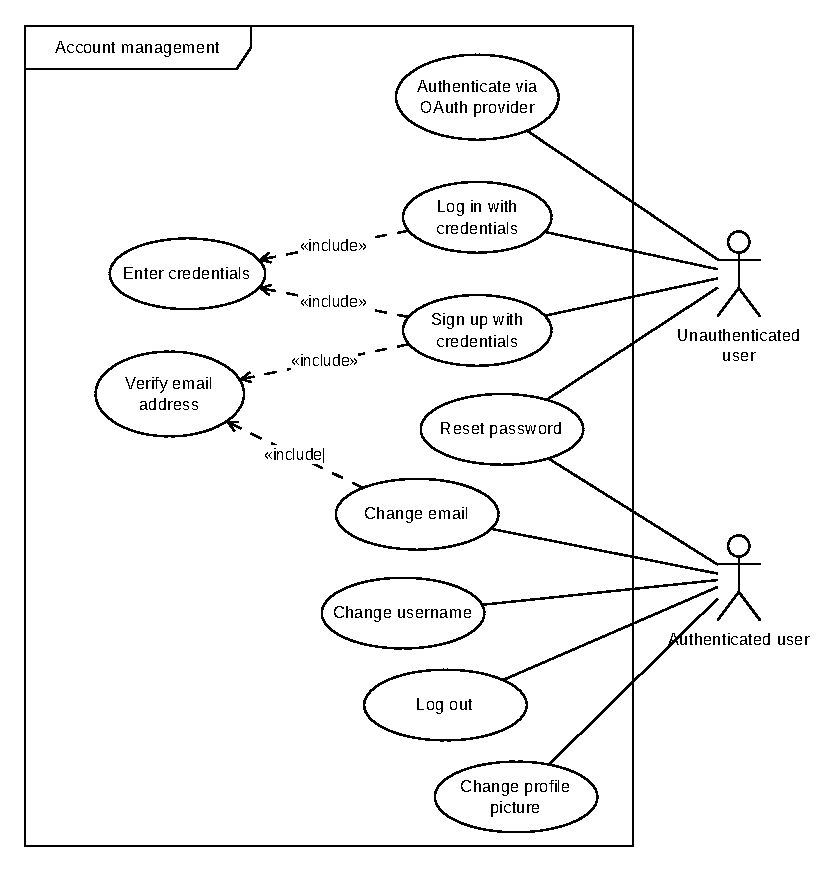
\includegraphics{figures/drawio/uc_account_management}
\caption{Use cases for managing the account.}
\label{fig:uc_account_management}
\end{figure}

Figure~\ref{fig:uc_account_management} shows the use cases that are related to account management and authorization of users. \newline
An \textbf{Authenticated} user is a user that is logged into an account and performs its actions in the context of that account.
An \textbf{Unauthenticated} user is a user that is not logged into an account. \newline
Both use cases \textbf{Sign up with credentials} and \textbf{Log in with credentials} require the user to \textbf{Enter credentials} for that specific account.
Furthermore, \textbf{Sign up with credentials} and \textbf{Change email} both result in the need for the user to \textbf{Verify the email address}.
Personal data change is performed with the use cases \textbf{Change username} and \textbf{Change profile picture}.
Additionally, authenticated users can \textbf{Log out} of the current account. \newline
Following, the use cases \textbf{Verify email address} (\ref{subsubsec:verify-email-address}), \textbf{Reset password} (\ref{subsubsec:reset-password}), and \textbf{Authenticate via \hyperref[def:oauth]{OAuth} provider} (\ref{subsubsec:authenticate-with-oauth}) are further expanded on.

\subsubsection{Verify email address}\label{subsubsec:verify-email-address}
\begin{figure}
	\centering
	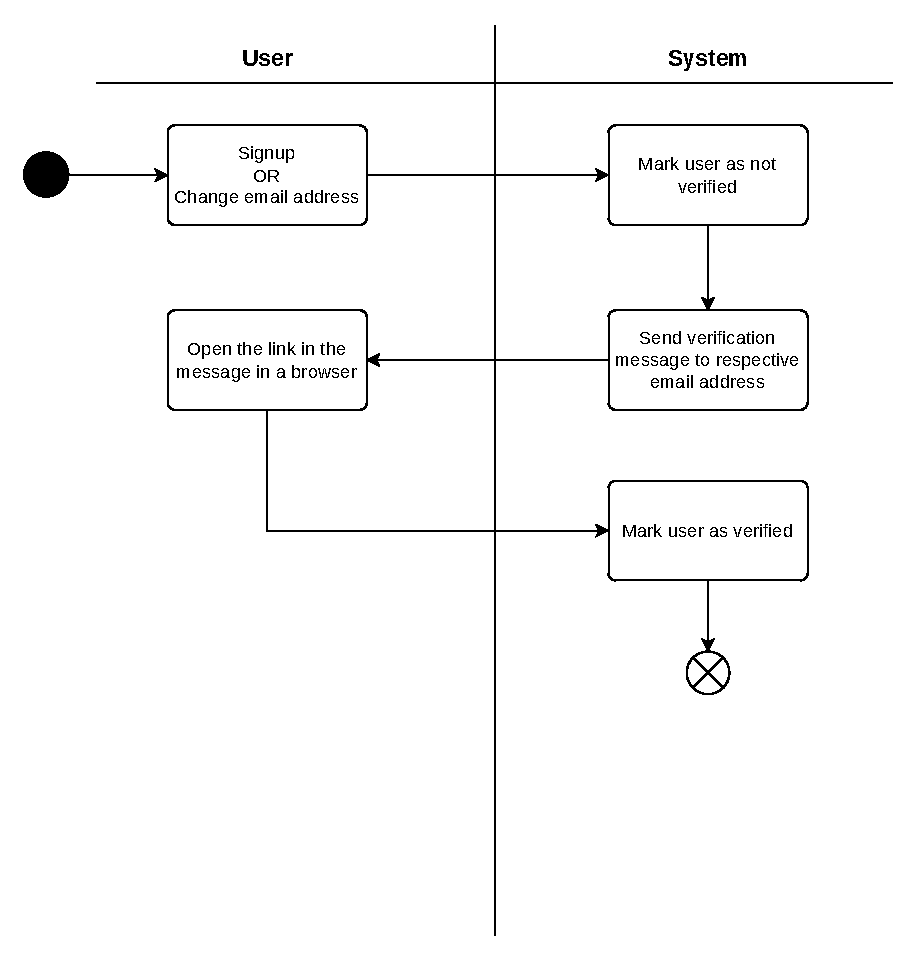
\includegraphics{figures/drawio/a_verify_email_address}
	\caption{Use case: Verify email address.}
	\label{fig:a_verify_email_address}
\end{figure}

Figure~\ref{fig:a_verify_email_address} shows the functions involved in performing the \textbf{Verify email address} use case. \newline
The use case is triggered either by a user signing up, or by changing the email address of their account.
The system sends a message to the new email address, which the user can use to verify their account.

\subsubsection{Reset password}\label{subsubsec:reset-password}
\begin{figure}
	\centering
	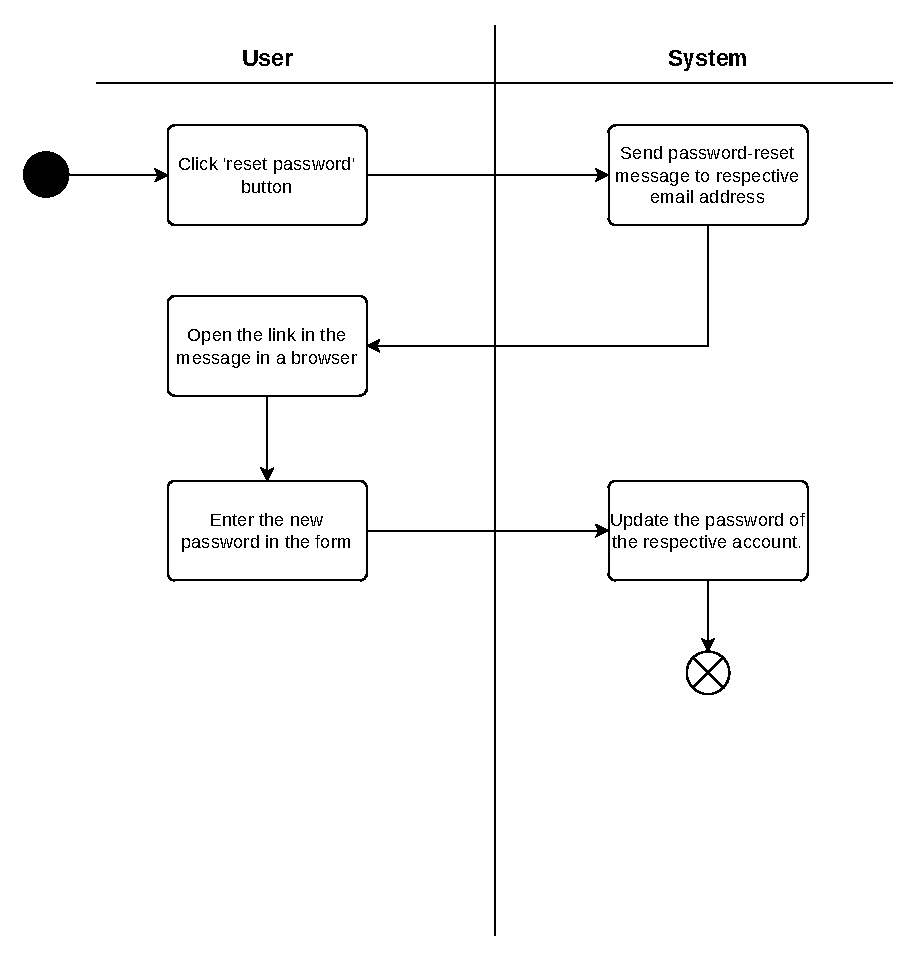
\includegraphics{figures/drawio/a_reset_password}
	\caption{Use case: Reset password.}
	\label{fig:a_reset_password}
\end{figure}

Figure~\ref{fig:a_reset_password} shows the functions involved in performing the \textbf{Reset password} use case. \newline
The use case is triggered actively by the user.
After that, the system sends a message to the user's email address, which contains a link where the user can enter the new password.
Finally, the user can authenticate with the new password.

\subsubsection{Authenticate via \hyperref[def:oauth]{OAuth} provider}\label{subsubsec:authenticate-with-oauth}
\begin{figure}
	\centering
	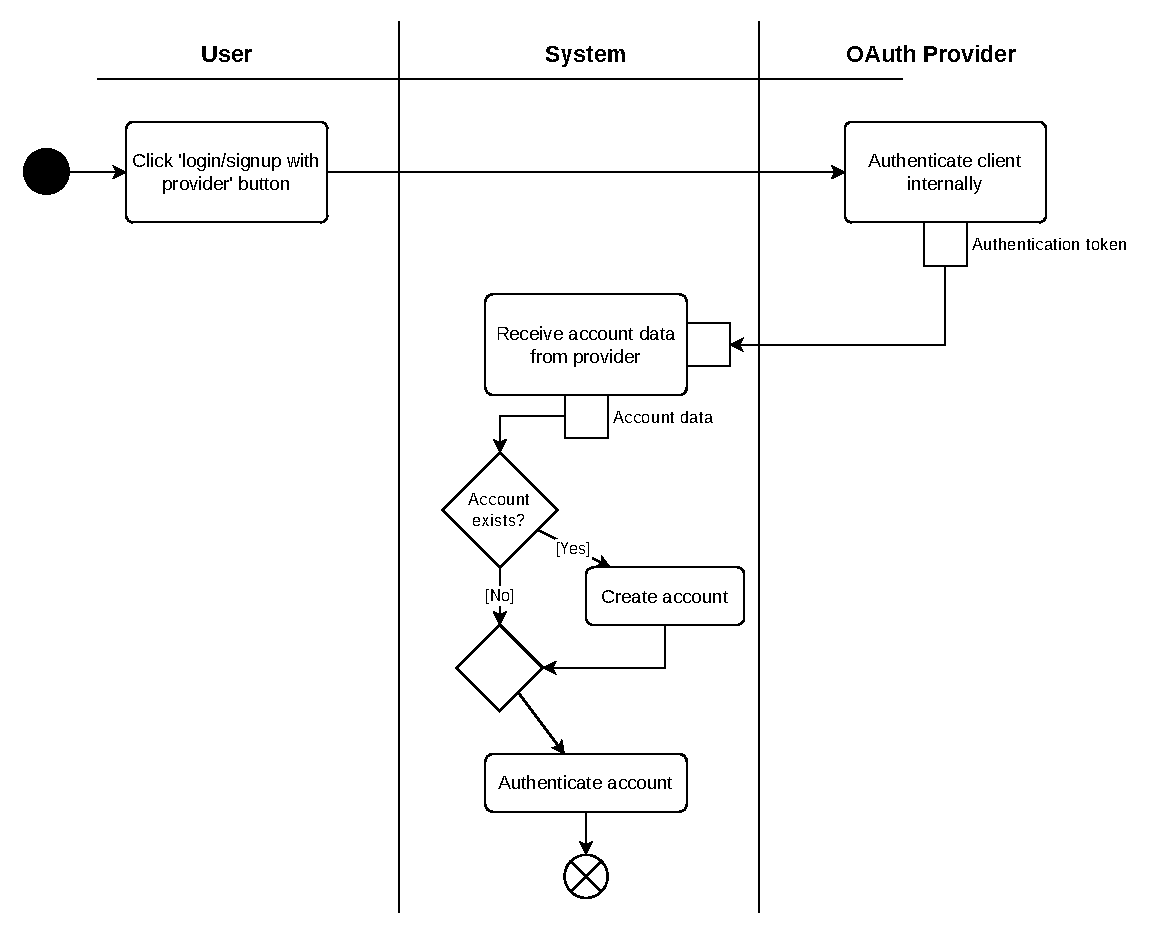
\includegraphics[width=\linewidth]{figures/drawio/a_auth_with_oauth}
	\caption{Use case: Authenticate via \hyperref[def:oauth]{OAuth} provider.}
	\label{fig:a_auth_with_oauth}
\end{figure}

Figure~\ref{fig:a_auth_with_oauth} shows the functions involved in performing the \textbf{Authenticate via \hyperref[def:oauth]{OAuth} provider} use case. \newline
This use case is triggered by a user selecting the \textit{\hyperref[def:oauth]{OAuth}} provider on the log-in/signup screen.
The authentication is handled by the provider.
This could be via credentials, using available cookies or other internal mechanisms.
After the internal authentication was performed, an access token is provided to the \textbf{CodeX} system, which it uses to connect the external account to a \textbf{CodeX} account, or create a new one if it doesn't yet exist.

\subsection{Conversations}

\begin{figure}
	\centering
	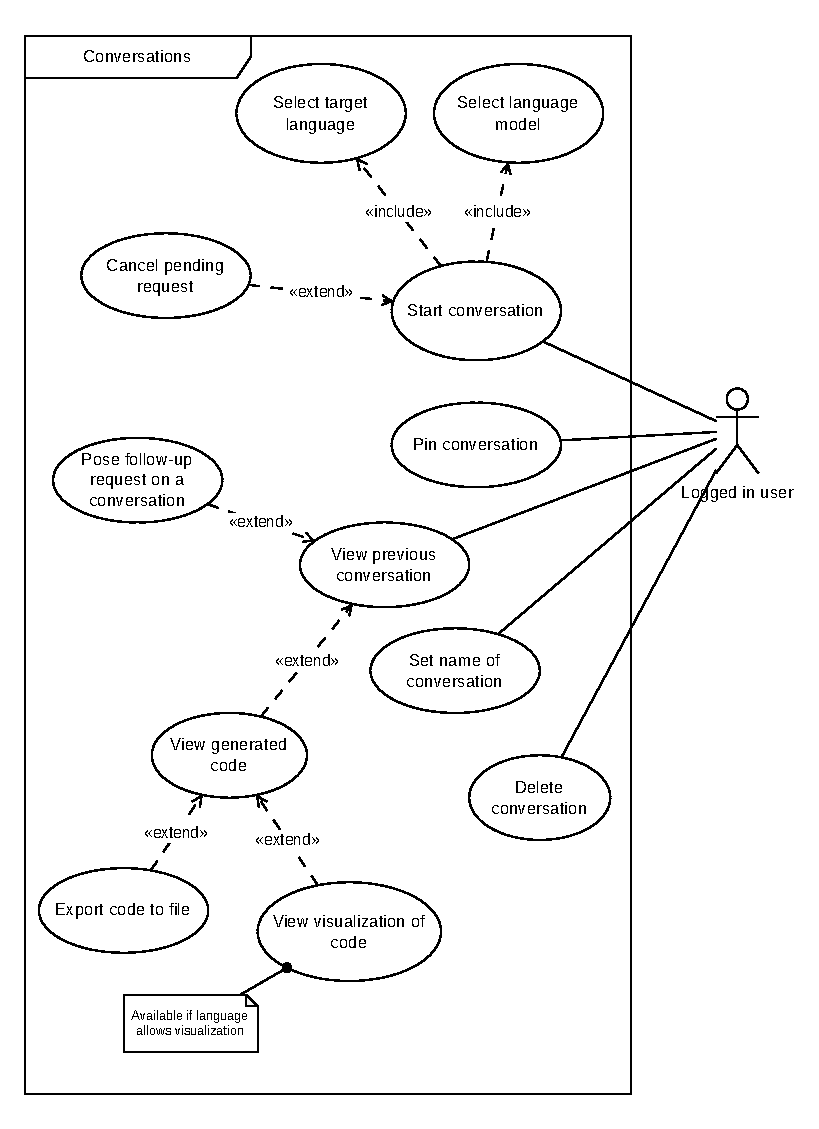
\includegraphics{figures/drawio/uc_conversations}
	\caption{Use cases for interacting with conversations.}
	\label{fig:uc_conversations}
\end{figure}

Figure~\ref{fig:uc_conversations} shows the use cases that describe how a user can interact with single or multiple conversations. \newline
In the list of all conversations, single ones can be \textbf{pinned to the top}, \textbf{assigned a name} or be \textbf{deleted}.
Users can also \textbf{View previous conversations} and \textbf{Pose follow-up questions on a conversation}.
When a request is pending, it can be \textbf{canceled}.
For an existing conversation, the user can \textbf{View the generated code} and optionally \textbf{Export the code to a file} or \textbf{View a visualization of the code}, if supported. \newline
The use-case \textbf{Start conversation} is further expanded on in \ref{subsubsec:start-conversation}.

\subsubsection{Start conversation}\label{subsubsec:start-conversation}
\begin{figure}
	\centering
	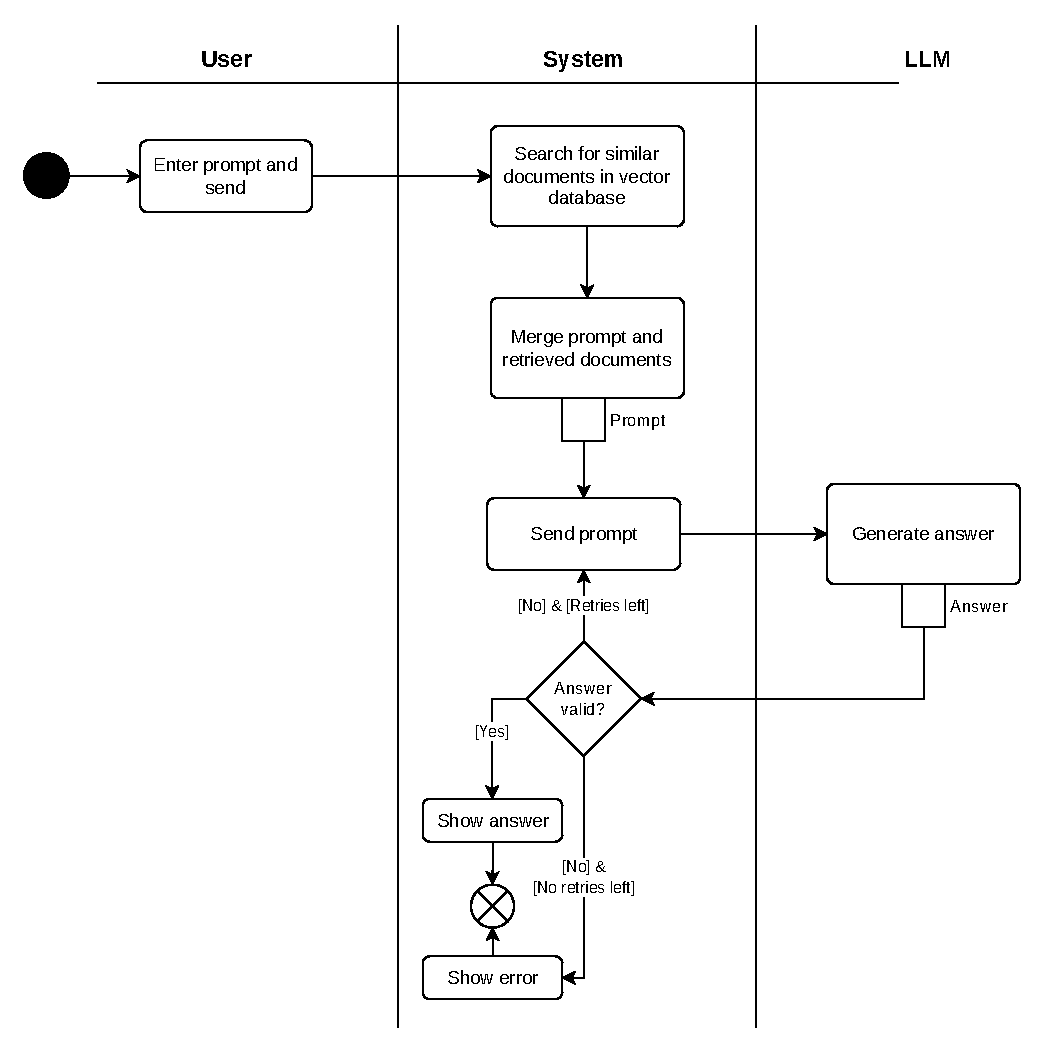
\includegraphics[width=\linewidth]{figures/drawio/a_start_conversation}
	\caption{Use case: Start conversation.}
	\label{fig:a_start_conversation}
\end{figure}

Figure~\ref{fig:a_start_conversation} shows the functions involved in performing the \textbf{Start conversation} use case. \newline
This use case is triggered by a user entering a prompt and sending it.
The system will associate the prompt with a list of documents retrieved from the vector database and merge it with the original prompt of the user.
This combined prompt is sent to the \textit{\hyperref[abr:LLM]{LLM}}, which in turn generates a response.
Depending on the target language, this answer is validated.
If the validation fails, the system retries the request several times and shows a response to the user.

\subsection{Admin Panel}

\begin{figure}
	\centering
	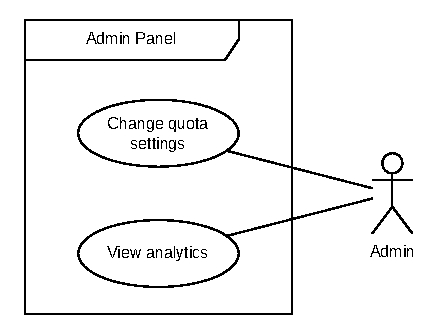
\includegraphics{figures/drawio/uc_admin_panel}
	\caption{Use cases for admin actions.}
	\label{fig:uc-admin-panel}
\end{figure}

Figure~\ref{fig:uc-admin-panel} shows the use cases that describe the actions that are specific to admins. \newline
Admins can \textbf{Change quota settings}, i.e.\ enabling/disabling quotas for specific roles and set the maximum number of requests.
Additionally, admins can view analytic data. \newline

\subsection{Settings}
\begin{figure}
	\centering
	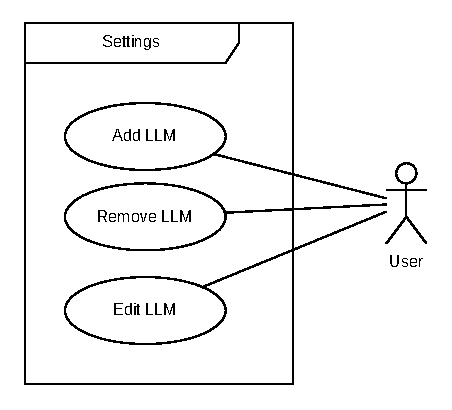
\includegraphics{figures/drawio/uc_settings}
	\caption{Use cases for settings.}
	\label{fig:uc-settings}
\end{figure}

Figure~\ref{fig:uc-settings} shows the use cases that describe the actions that can be performed in the settings section. \newline
Users can \textbf{add}, \textbf{edit} and \textbf{remove} \textit{\hyperref[abr:LLM]{LLM}} models.

\subsection{Miscellaneous}

\begin{figure}
	\centering
	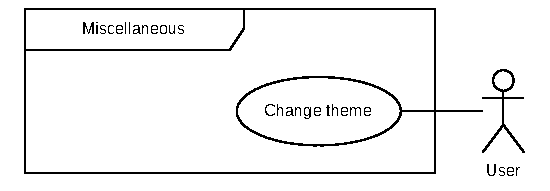
\includegraphics{figures/drawio/uc_miscellaneous}
	\caption{Miscellaneous use cases.}
	\label{fig:uc_miscellaneous}
\end{figure}

Figure~\ref{fig:uc_miscellaneous} contains miscellaneous use cases that don't fit in other categories. \newline
\textbf{Change theme} refers to the action of a user being able to toggle the color theme of the user interface between light and dark mode.
%!TEX root = ../Pflichtenheft.tex

\chapter{Product functions}
In the following, the product functions are declared. \newline
Product functions are a more concrete description of the functions used in the use cases.
Each product function will be assigned to one or multiple must-, should- or could requirements.
\newline
\newline
\textbf{Note:} The actors follow a hierarchical relation defined as \textit{\hyperref[def:guest]{Guest} < \hyperref[def:user]{User} < \hyperref[def:admin]{Admin}}. 
This means that if a product function is assigned to a certain actor (e.g., \textit{\hyperref[def:guest]{Guest}}), 
it can also be performed by all actors of higher levels (in this case, \textit{\hyperref[def:user]{User}} and \textit{\hyperref[def:admin]{Admin}}).

\vspace{3.5em}

\begin{function}{10}{Authenticate via \hyperref[def:oauth]{OAuth} provider}
	\item[Use case:] Authenticate via \hyperref[def:oauth]{OAuth} provider
	\item[Criteria:]~\ref{RC10}
	\item[Target:] The user is logged into an account, and was authenticated via an external provider like \textit{Google}.
	\item[Precondition:] The user is not logged in.
	\item[Postcondition failure:] The user is still logged out, or no new account was created.
	\item[Actors:] \hyperref[def:guest]{Guest}
	\item[Trigger:] The user clicks the option to login/signup with an external provider on the Login or Signup screen.
	\item[Description:] ~
	\begin{enumerate}
		\item User clicks option to authenticate with external provider.
		\item User authenticates for the external provider.
		\item System creates session or new account based on the token from the external provider.
		\item User is authenticated and redirected to the main page.
	\end{enumerate}
	See also~\ref{subsubsec:authenticate-with-oauth}.
\end{function}

\newpage
\vspace{2.0em}

\begin{function}{20}{Log in with credentials}
	\item[Use case:] Log in with credentials
	\item[Criteria:]~\ref{RS3}
	\item[Target:] The user is logged into an existing account.
	\item[Precondition:] The user is not logged in.
	\item[Postcondition failure:] The user is still logged out.
	\item[Actors:] \hyperref[def:guest]{Guest}
	\item[Trigger:] The user clicks the login button on the Login screen.
	\item[Description:] ~
	\begin{enumerate}
		\item User enters credentials on the Login screen.
		\item User clicks the login button on the Login screen.
		\item System validates the credentials, authenticated the user and redirects to the main page.
	\end{enumerate}
\end{function}
\vspace{2.0em}

\begin{function}{30}{Sign up with credentials}
	\item[Use case:] Sign up with credentials
	\item[Criteria:]~\ref{RS3},~\ref{RS4}
	\item[Target:] The user is logged into a new account.
	\item[Precondition:] The user is not logged in.
	\item[Postcondition failure:] The user is still logged out, or no account was created.
	\item[Actors:] \hyperref[def:guest]{Guest}
	\item[Trigger:] The user clicks the signup button on the Signup screen.
	\item[Description:] ~
\begin{enumerate}
	\item User enters new credentials on the Signup screen.
	\item User clicks the signup button on the Signup screen.
	\item System creates new account and requires the user to verify the email address.
\end{enumerate}
\end{function}
\newpage
\vspace{2.0em}

\begin{function}{40}{Change email}
	\item[Use case:] Change email
	\item[Criteria:]~\ref{RS5}
	\item[Target:] The email address of the user is updated and the user marked as unverified.
	\item[Postcondition failure:] The email address of the user is still the old one.
	\item[Actors:] \hyperref[def:user]{User}
	\item[Trigger:] The user clicks the change email button in the account dialog.
	\item[Description:] ~
	\begin{enumerate}
		\item The user enters the new email address in the change email dialog.
		\item The system ensures the email is not yet used.
		\item The system updates the email and sets the user to unverified.
		\item The user is logged out.
	\end{enumerate}
\end{function}
\vspace{2.0em}

\begin{function}{50}{Verify email address}
	\item[Use case:] Verify email address
	\item[Criteria:]~\ref{RC9}
	\item[Target:] The email address of the user is verified.
	\item[Precondition:] The email address of the user is not yet verified.
	\item[Postcondition failure:] The email address of the user is not verified.
	\item[Actors:] \hyperref[def:guest]{Guest}
	\item[Trigger:] The user signs up or changes the email address.
	\item[Description:] ~
	\begin{enumerate}
		\item A message is sent to the users email address.
		\item The user clicks the link contained in the message.
		\item The system sets the email address of the user to validated.
	\end{enumerate}
	See also~\ref{subsubsec:verify-email-address}.
\end{function}
\newpage
\vspace{2.0em}


\begin{function}{60}{Reset password}
	\item[Use case:] Reset password
	\item[Criteria:]~\ref{RS6},~\ref{RC9}
	\item[Target:] The password of the account is changed.
	\item[Postcondition failure:] The password of the account was not changed.
	\item[Actors:] \hyperref[def:user]{User}
	\item[Trigger:] The user clicks the reset password button in the account dialog or the login screen.
	\item[Description:] ~
	\begin{enumerate}
		\item The user requests the password reset message to be sent to their email address.
		\item The user clicks the link in the message.
		\item The user enters the new password in the reset password screen.
		\item The system updates the password of the account.
	\end{enumerate}
	See also~\ref{subsubsec:reset-password}.
\end{function}
\vspace{2.0em}

\begin{function}{70}{Change username}
	\item[Use case:] Change username
	\item[Criteria:]~\ref{RS5}
	\item[Target:] The username of the account is changed.
	\item[Postcondition failure:] The username of the account was not changed.
	\item[Actors:] \hyperref[def:user]{User}
	\item[Trigger:] The user clicks the change username button in the change username dialog.
	\item[Description:] ~
	\begin{enumerate}
		\item The user enters the new username in the change username dialog.
		\item The user clicks the confirm button in the change username dialog.
		\item The system updates the username of the account.
	\end{enumerate}
\end{function}
\newpage
\vspace{2.0em}

\begin{function}{80}{Log out}
	\item[Use case:] Log out
	\item[Criteria:]~\ref{RS3}
	\item[Target:] The current session of the user is invalidated.
	\item[Postcondition failure:] The current session of the user is still active.
	\item[Actors:] \hyperref[def:user]{User}
	\item[Trigger:] The user clicks the logout button in the account dialog.
	\item[Description:] ~
	\begin{enumerate}
		\item The user clicks the logout button in the account dialog.
		\item The system invalidates the current session of the user.
	\end{enumerate}
\end{function}
\vspace{2.0em}

\begin{function}{90}{Change profile picture}
	\item[Use case:] Change profile picture
	\item[Criteria:]~\ref{RC17}
	\item[Target:] The profile picture of the account is changed.
	\item[Postcondition failure:] The profile picture of the account is still the old one.
	\item[Actors:] \hyperref[def:user]{User}
	\item[Trigger:] The user clicks the profile picture in the account dialog.
	\item[Description:] ~
	\begin{enumerate}
		\item The user clicks the profile picture in the account dialog.
		\item The browser opens a file picker that lets the user pick an image file.
		\item The image file is sent to the system, which updates the profile picture of the account.
	\end{enumerate}
\end{function}
\vspace{2.0em}

\begin{function}{100}{Start conversation}
	\item[Use case:] Start conversation
	\item[Criteria:]~\ref{RM1},~\ref{RM5},~\ref{RS2},~\ref{RS7},~\ref{RS8},~\ref{RM6},~\ref{RC1},~\ref{RC14}
	\item[Target:] A new conversation is started by sending an initial code description to an \textit{LLM}.
	\item[Postcondition failure:] No new conversation is started, or no code was generated.
	\item[Actors:] \hyperref[def:guest]{Guest}
	\item[Trigger:] The user sent a prompt from the main page.
	\item[Description:] ~
	\begin{enumerate}
		\item The user sent a prompt from the main page.
		\item The system augments the prompt using the documents stored in the vector database.
		\item Until a validated response is received, or until a maximum number of reties has been reached, the system sends the augmented prompt to the \textit{LLM}.
		\item The code, or an error, is presented to the user.
	\end{enumerate}
	See also~\ref{subsubsec:start-conversation}.
\end{function}
\vspace{2.0em}

\begin{function}{110}{Select target language}
	\item[Use case:] Select target language
	\item[Criteria:]~\ref{RM2},~\ref{RC3}
	\item[Target:] A target language was selected for the coming conversation.
	\item[Postcondition failure:] No target language was selected.
	\item[Actors:] \hyperref[def:guest]{Guest}
	\item[Trigger:] The user selected a target language on the main page.
	\item[Description:] ~
	The user selects a target language from the language dropdown on the main page.
\end{function}
\vspace{2.0em}

\begin{function}{120}{Select language model}
	\item[Use case:] Select language model
	\item[Criteria:]~\ref{RM7}
	\item[Target:] A language model was selected for the coming conversation.
	\item[Postcondition failure:] No language model was selected.
	\item[Actors:] \hyperref[def:guest]{Guest}
	\item[Trigger:] The user selected a language model on the main page.
	\item[Description:] ~
	The user selects a language model from the language dropdown on the main page.
\end{function}
\vspace{2.0em}

\begin{function}{130}{Add or update language model}
	\item[Use case:] Add LLM/Update LLM
	\item[Criteria:]~\ref{RM7}
	\item[Target:] An LLM was added or updated.
	\item[Postcondition failure:] The LLM was not created or updated.
	\item[Actors:] \hyperref[def:guest]{Guest}
	\item[Trigger:] The user visited the settings view.
	\item[Description:] ~
	The user either adds a new LLM configuration by entering the name and \textit{URL}, or updates either of the attributes.
\end{function}

\begin{function}{140}{Delete language model}
	\item[Use case:] Delete LLM
	\item[Criteria:]~\ref{RM7}
	\item[Target:] An LLM configuration was deleted.
	\item[Postcondition failure:] The LLM config still exists.
	\item[Actors:] \hyperref[def:guest]{Guest}
	\item[Trigger:] The user visited the settings view.
	\item[Description:] ~
	The user selects the LLM config to delete, and clicks the delete button.
\end{function}
\vspace{2.0em}

\vspace{2.0em}

\begin{function}{150}{Pin conversation}
	\item[Use case:] Pin conversation
	\item[Criteria:]~\ref{RC8}
	\item[Target:] A conversation was pinned.
	\item[Postcondition failure:] The conversation was not pinned.
	\item[Actors:] \hyperref[def:user]{User}
	\item[Trigger:] The user hovers over a conversation on the navigation bar on the main page.
	\item[Description:] ~
	\begin{enumerate}
	    \item The user opens the context menu for a conversation on the left sidebar.
		\item The user clicks the pin menu option on the menu.
	\end{enumerate}
\end{function}
\vspace{1.5em}

\begin{function}{160}{View previous conversation}
	\item[Use case:] View previous conversation, View visualization of code
	\item[Criteria:]~\ref{RM3},~\ref{RS1},~\ref{RS7},~\ref{RS9},~\ref{RC2},~\ref{RC7},~\ref{RC13}
	\item[Target:] The user observed and performed actions on a conversation.
	\item[Postcondition failure:] The conversation was not shown.
	\item[Actors:] \hyperref[def:user]{User}
	\item[Trigger:] The user selects a conversation from the left sidebar or waits for a conversation to be finished.
	\item[Description:] ~
	The user observes the code that was generated by the \textit{LLM}. \newline
	If the target language allows visualization, the user can select to view the visualization.
	The user can pose follow-up prompts on the conversations.
\end{function}
\vspace{1.5em}

\begin{function}{170}{Export code to file}
	\item[Use case:] Export code to file
	\item[Criteria:]~\ref{RM1},~\ref{RC15}
	\item[Target:] The generated code was downloaded as a file.
	\item[Postcondition failure:] The file was not downloaded.
	\item[Actors:] \hyperref[def:user]{User}
	\item[Trigger:] The user clicks the download button on a code snipped of a conversation.
	\item[Description:] ~
	The user clicks the download button on a code snipped, and the browser loads the file into the users downloads directory.
\end{function}
\vspace{2.0em}

\begin{function}{180}{Change theme}
	\item[Use case:] Change theme
	\item[Criteria:]~\ref{RC11}
	\item[Target:] The theme of the interface is toggled.
	\item[Postcondition failure:] The theme is not toggled.
	\item[Actors:] \hyperref[def:guest]{Guest}
	\item[Trigger:] The user clicks the theme toggle button in the sidebar.
	\item[Description:] ~
	The user clicks the theme toggle button in the sidebar.
	The web interface inverts its color scheme.
\end{function}
\vspace{2.0em}

\begin{function}{190}{Set name of conversation}
	\item[Use case:] Set name of conversation
	\item[Criteria:]~\ref{RM4}
	\item[Target:] The name of the conversation is changed.
	\item[Postcondition failure:] The name of the conversation is not changed.
	\item[Actors:] \hyperref[def:user]{User}
	\item[Trigger:] The user selects the rename option in the conversation menu.
	\item[Description:] ~
	The user selects the rename option in the conversation context menu.
	After that, the name field of the conversation becomes editable, and the user enters the new name.
\end{function}
\vspace{2.0em}

\begin{function}{200}{Delete conversation}
	\item[Use case:] Delete conversation
	\item[Criteria:]~\ref{RS10}
	\item[Target:] The conversation is deleted.
	\item[Postcondition failure:] The conversation is not deleted.
	\item[Actors:] \hyperref[def:user]{User}
	\item[Trigger:] The user selects the delete option in the conversation menu.
	\item[Description:] ~
	The user selects the delete option in the conversation context menu.
	The system marks the conversation as deleted and hides it from the user.
\end{function}
\vspace{2.0em}

\begin{function}{210}{Change quota settings}
	\item[Use case:] Change quota settings
	\item[Criteria:]~\ref{RC4},~\ref{RC5}
	\item[Target:] The quota settings are changed.
	\item[Postcondition failure:] The quota settings are not changed.
	\item[Actors:] \hyperref[def:admin]{Admin}
	\item[Trigger:] The user updates the quota values on the admin panel.
	\item[Description:] ~
	The user updates the quota settings on the admin panel.
\end{function}
\vspace{2.0em}

\begin{function}{220}{View analytics}
	\item[Use case:] View analytics
	\item[Criteria:]~\ref{RC4},~\ref{RC16}
	\item[Target:] The analytics have been displayed.
	\item[Postcondition failure:] The analytics were not displayed.
	\item[Actors:] \hyperref[def:admin]{Admin}
	\item[Trigger:] The user visits the admin panel.
	\item[Description:] ~
	The admin panel displays some analytics about the usage of the server.
\end{function}

\vspace{2.0em}
\begin{function}{230}{Multilingual web interface}
	\item[Use case:] Multilingual web interface
	\item[Criteria:]~\ref{RC6}
	\item[Target:] The web interface is available in multiple languages (at least German and English).
	\item[Postcondition failure:] The web interface is only available in one language.
	\item[Actors:] \hyperref[def:guest]{Guest}
	\item[Trigger:] The user changes the language in the web interface settings.
	\item[Description:] ~
	The web interface supports multiple languages. Users can switch the displayed language between at least German and English through the interface settings.
\end{function}
%!TEX root = ../Pflichtenheft.tex

\chapter{Product Data}
The following describes what external data is persisted by the system.

\begin{data}{10}{Data per account}
	\begin{itemize}
		\item Date of signup
		\item Username
		\item Email
		\item One-Way encrypted password
		\item Profile picture
		\item Role
		\item UI theme
		\item Email verification status
		\item Language model configurations:
		\begin{itemize}
				  \item Name
				  \item OpenAPI endpoint
		\end{itemize}
	\end{itemize}
\end{data}

\begin{data}{20}{Authentication Data}
	\begin{itemize}
		\item Active, expired and invalidated sessions
	\end{itemize}
\end{data}

\begin{data}{30}{Data per conversation}
	\begin{itemize}
		\item Date of creation
		\item Name
		\item User-sent requests
		\item LLM-sent responses
		\item Owner account
		\item Used language model
		\item Used target language
		\item Whether it is pinned
		\item Validation result
	\end{itemize}
\end{data}

\begin{data}{40}{Global Data}
	\begin{itemize}
		\item Maximum requests per role
	\end{itemize}
\end{data}

%!TEX root = ../Pflichtenheft.tex

% Kapitel 6
%-------------------------------------------------------------------------------

\chapter{Quality criteria}
\textbf{Quality criteria} describe the way that the proposed must-, should- and could criteria get implemented. Quality criteria are not visible to the immediate user, but deal with topics like legal regulations, data privacy, security or safety.

\qualityReq{10}{\hyperref[abr:SQL]{SQL} injection or any other form of database injection \textbf{must not} be possible.}
\qualityReq{20}{No personally identifiable information (\textit{\hyperref[abr:PII]{PII}}) must be shared with external services.}
\qualityReq{30}{The code generation must not take longer than 20 seconds.}
\qualityReq{40}{All user passwords should only be persisted using a secure, one-way hashing algorithm.}
\qualityReq{50}{The system should limit concurrent requests per user to prevent overloading the server.}
\qualityReq{60}{All server-side logging should be performed using a logging framework to ensure structured logs, maintainability, and effective debugging.}
\qualityReq{70}{The frontend should handle all operations without runtime errors, ensuring that users do not encounter unhandled exceptions or crashes during normal use.} 
\qualityReq{80}{The frontend should not produce any errors in the browser console during normal operation, ensuring a stable and reliable user experience.}
\qualityReq{90}{All communication between frontend and backend should be encrypted (e.g., using \hyperref[abr:HTTP]{HTTP}S) to ensure data security.}
\qualityReq{100}{The system could be deployable using containerization, such as \textit{Docker}.}
\qualityReq{110}{The system could allow integration with \hyperref[abr:CI/CD]{CI/CD} pipelines to automatically test or deploy generated code.}
\qualityReq{120}{The interface of the system should be responsive on the display sizes \textit{Mobile Phone}, \textit{Tablet} and \textit{Desktop}. It should also be accessible.}
\qualityReq{130}{The \textit{\hyperref[abr:LLM]{LLM}} and \textit{Database} should be stored on a secure server and can only be accessed by authorized actors.}
%!TEX root = ../Pflichtenheft.tex

\chapter{Graphical User Interface}\label{ch:ui}
This chapter provides an overview of the \textit{\hyperref[abr:GUI]{GUI}} that is provided by the the system. \newline
While the designed interface is detailed and has been created implementation-near, it is not indented to be a pixel-perfect replica of the interface, but rather an example of how the interface may look like.
Aspects like spacing, texts, colors or layout choices are subject to change. \newline
Sections \ref{sec:navigation}, \ref{sec:screens} and \ref{sec:modals} present screens and modals for the web-interface, while section \ref{sec:email} presents the design of the emails sent to the user.

\section{Navigation}\label{sec:navigation}
The user will be able to navigate around the app using a so-called \textit{Navigation Drawer} \footnote{https://m3.material.io/components/navigation-drawer/overview}. \newline
A navigation drawer is a section of a web-app that is usually aligned on the start of the main layout (horizontally) and gives a user a list of navigation destinations to jump to. \newline
In a scenario of a wide viewport, like a \textit{Desktop} or \textit{Tablet} device, this navigation rail will always be visible to the user. \newline
In the scenario of a narrow viewport, like a \textit{Mobile}, this navigation rail will be only visible after being toggled by the user, using a toggle-button at the top of the screen.
Due to this, the navigation rail won't be visible on the UI-drafts for mobile screens.
Figure~\ref{fig:ui_d_mobile_navigation_drawer_overlay} shows this overlay of the navigation drawer on mobile devices.

\begin{figure}
    \centering
    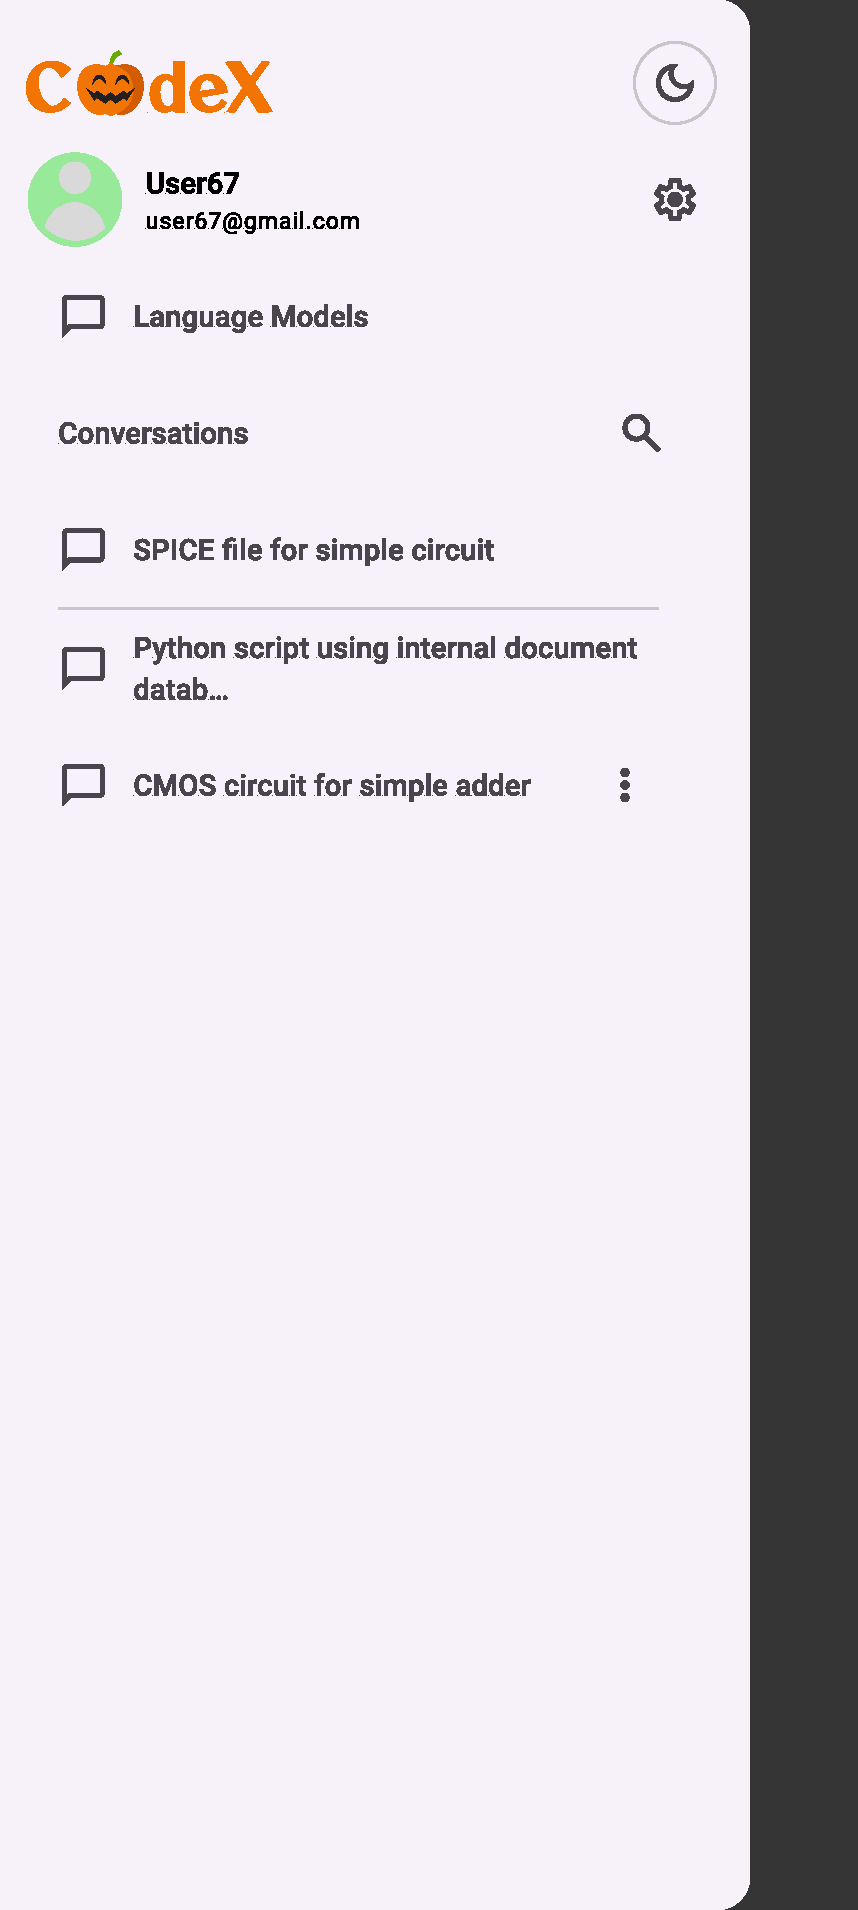
\includegraphics[width=5cm]{figures/ui/mobile/Navbar_Preview}
    \caption{\hyperref[abr:GUI]{GUI}: Navigation drawer overlay on mobile devices}
    \label{fig:ui_d_mobile_navigation_drawer_overlay}
\end{figure}

\section{Screens}\label{sec:screens}
Due to the different proportions of the possible screen sizes, each screen is presented as a \textit{Desktop} and \textit{Mobile} variant.
Whenever there is a link to a specific screen, the two variants are specified like the following: \texttt{<desktop\_variant>/<mobile\_variant>}.

\subsection{Conversation screen}
The conversation screen is the main screen of the app.
Here, the user has access to a sidebar that contains the previous conversations, as well as options to visit the account settings and toggle the theme of the app. \newline
The main content is the interface to create requests.
Before sending a request (\ref{fig:ui_d_conversation_screen_initial}/\ref{fig:ui_m_conversation_screen_initial}), the user can select the target language and \textit{\hyperref[abr:LLM]{LLM}}.
While the request is processing (\ref{fig:ui_d_conversation_screen_loading}/\ref{fig:ui_m_conversation_screen_loading}), a progress bar is shown.
When the request is finished, the user can either see the raw code (\ref{fig:ui_d_conversation_screen_not_visualized}/\ref{fig:ui_m_conversation_screen_not_visualized}) or visualize the code (\ref{fig:ui_d_conversation_screen_visualized}/\ref{fig:ui_m_conversation_screen_visualized}) if available for the specific language.

\begin{figure}
    \centering
    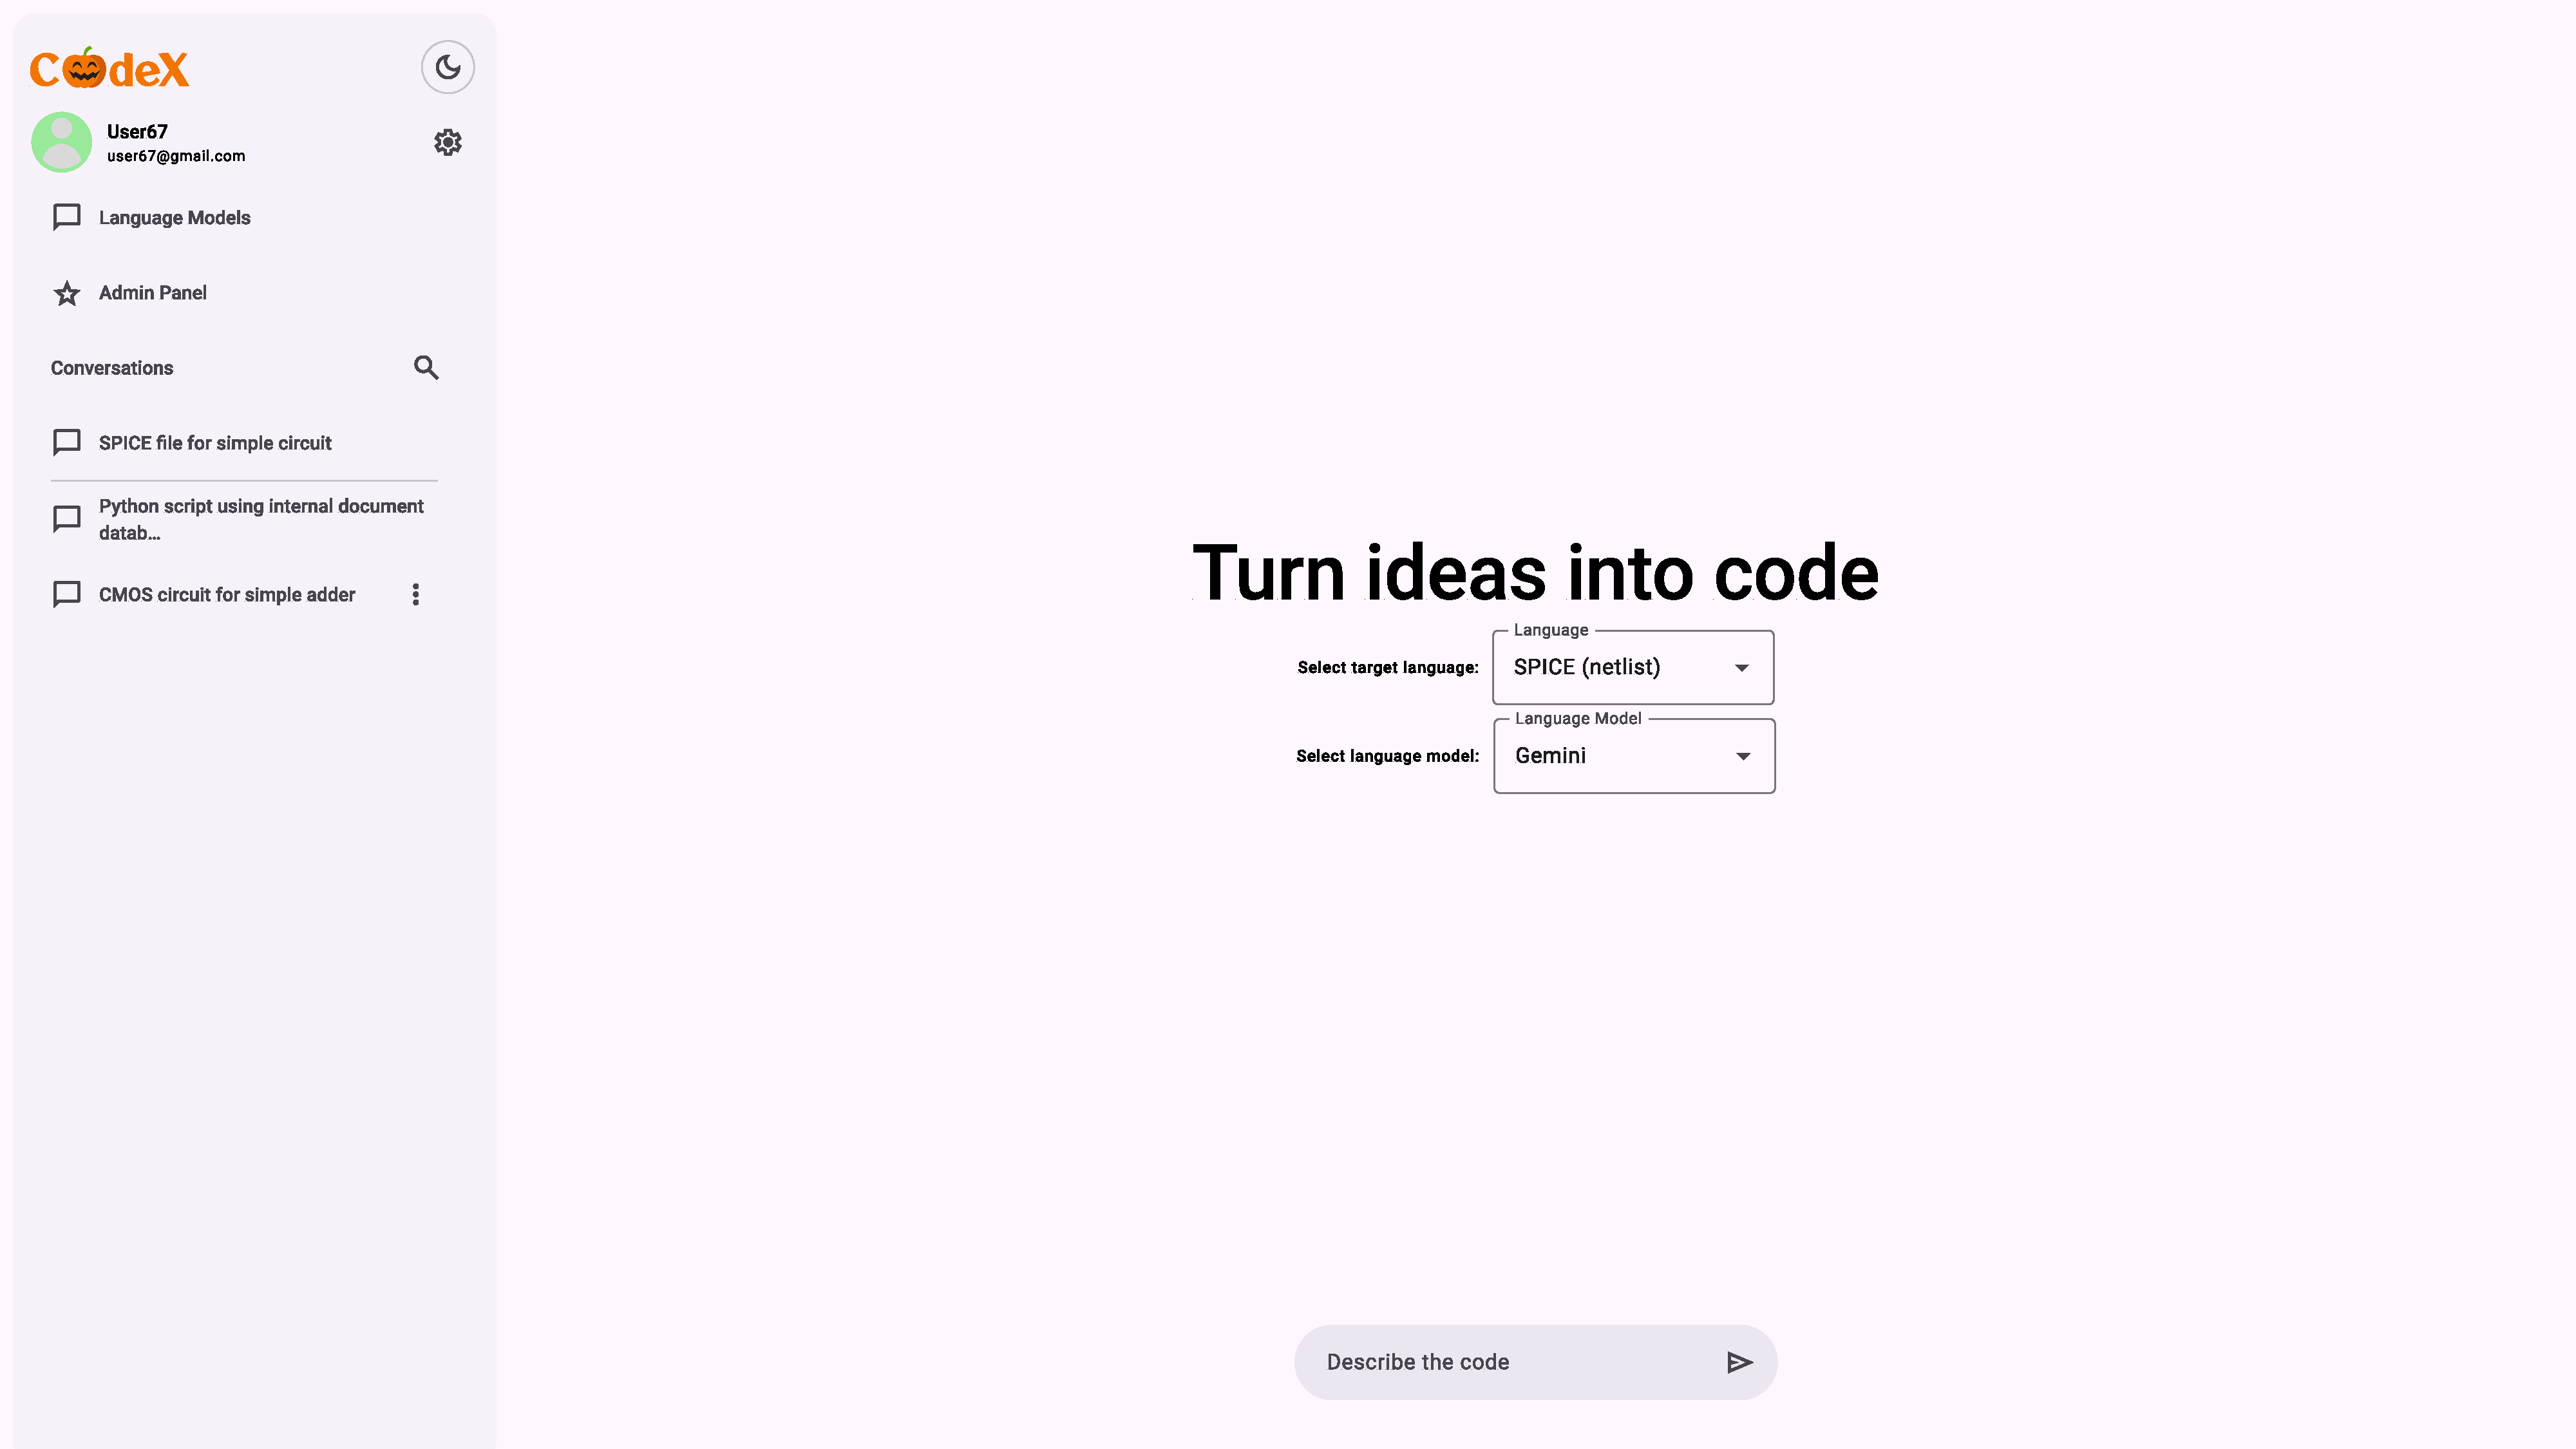
\includegraphics[width=\linewidth]{figures/ui/desktop/Conversation_Screen initial}
    \caption{\hyperref[abr:GUI]{GUI}: Conversation screen before request}
    \label{fig:ui_d_conversation_screen_initial}
\end{figure}
\begin{figure}
    \centering
    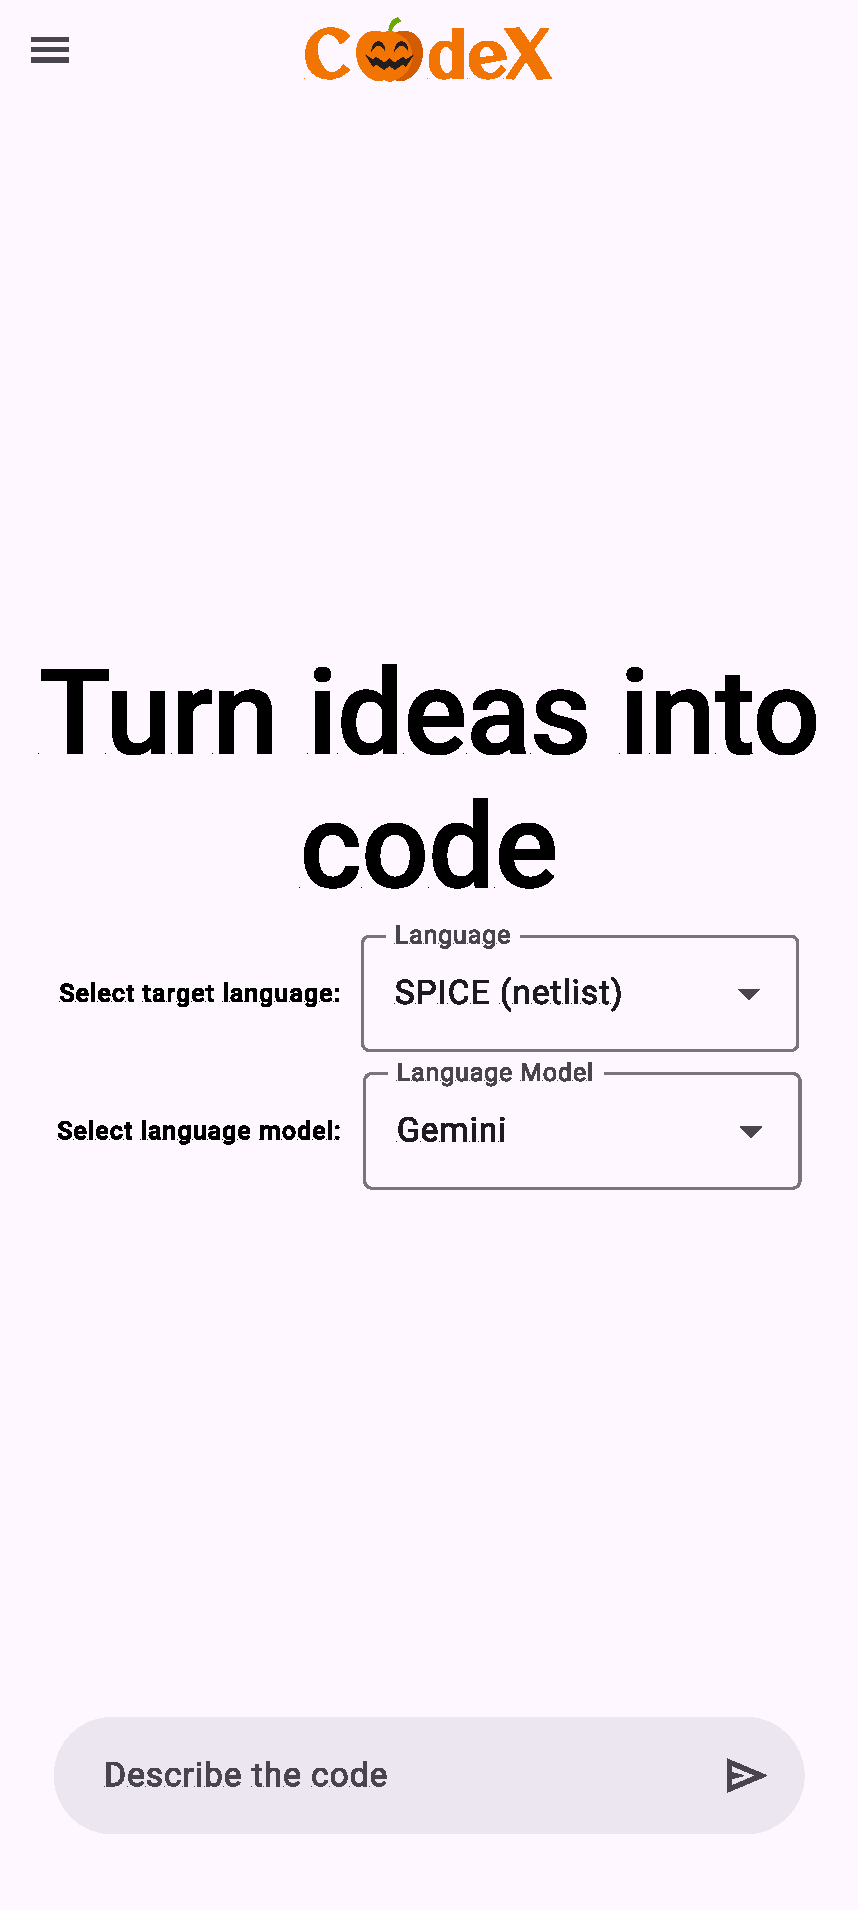
\includegraphics[width=5cm]{figures/ui/mobile/Conversation_Screen initial}
    \caption{\hyperref[abr:GUI]{GUI}: Conversation screen before request (mobile)}
    \label{fig:ui_m_conversation_screen_initial}
\end{figure}

\begin{figure}
    \centering
    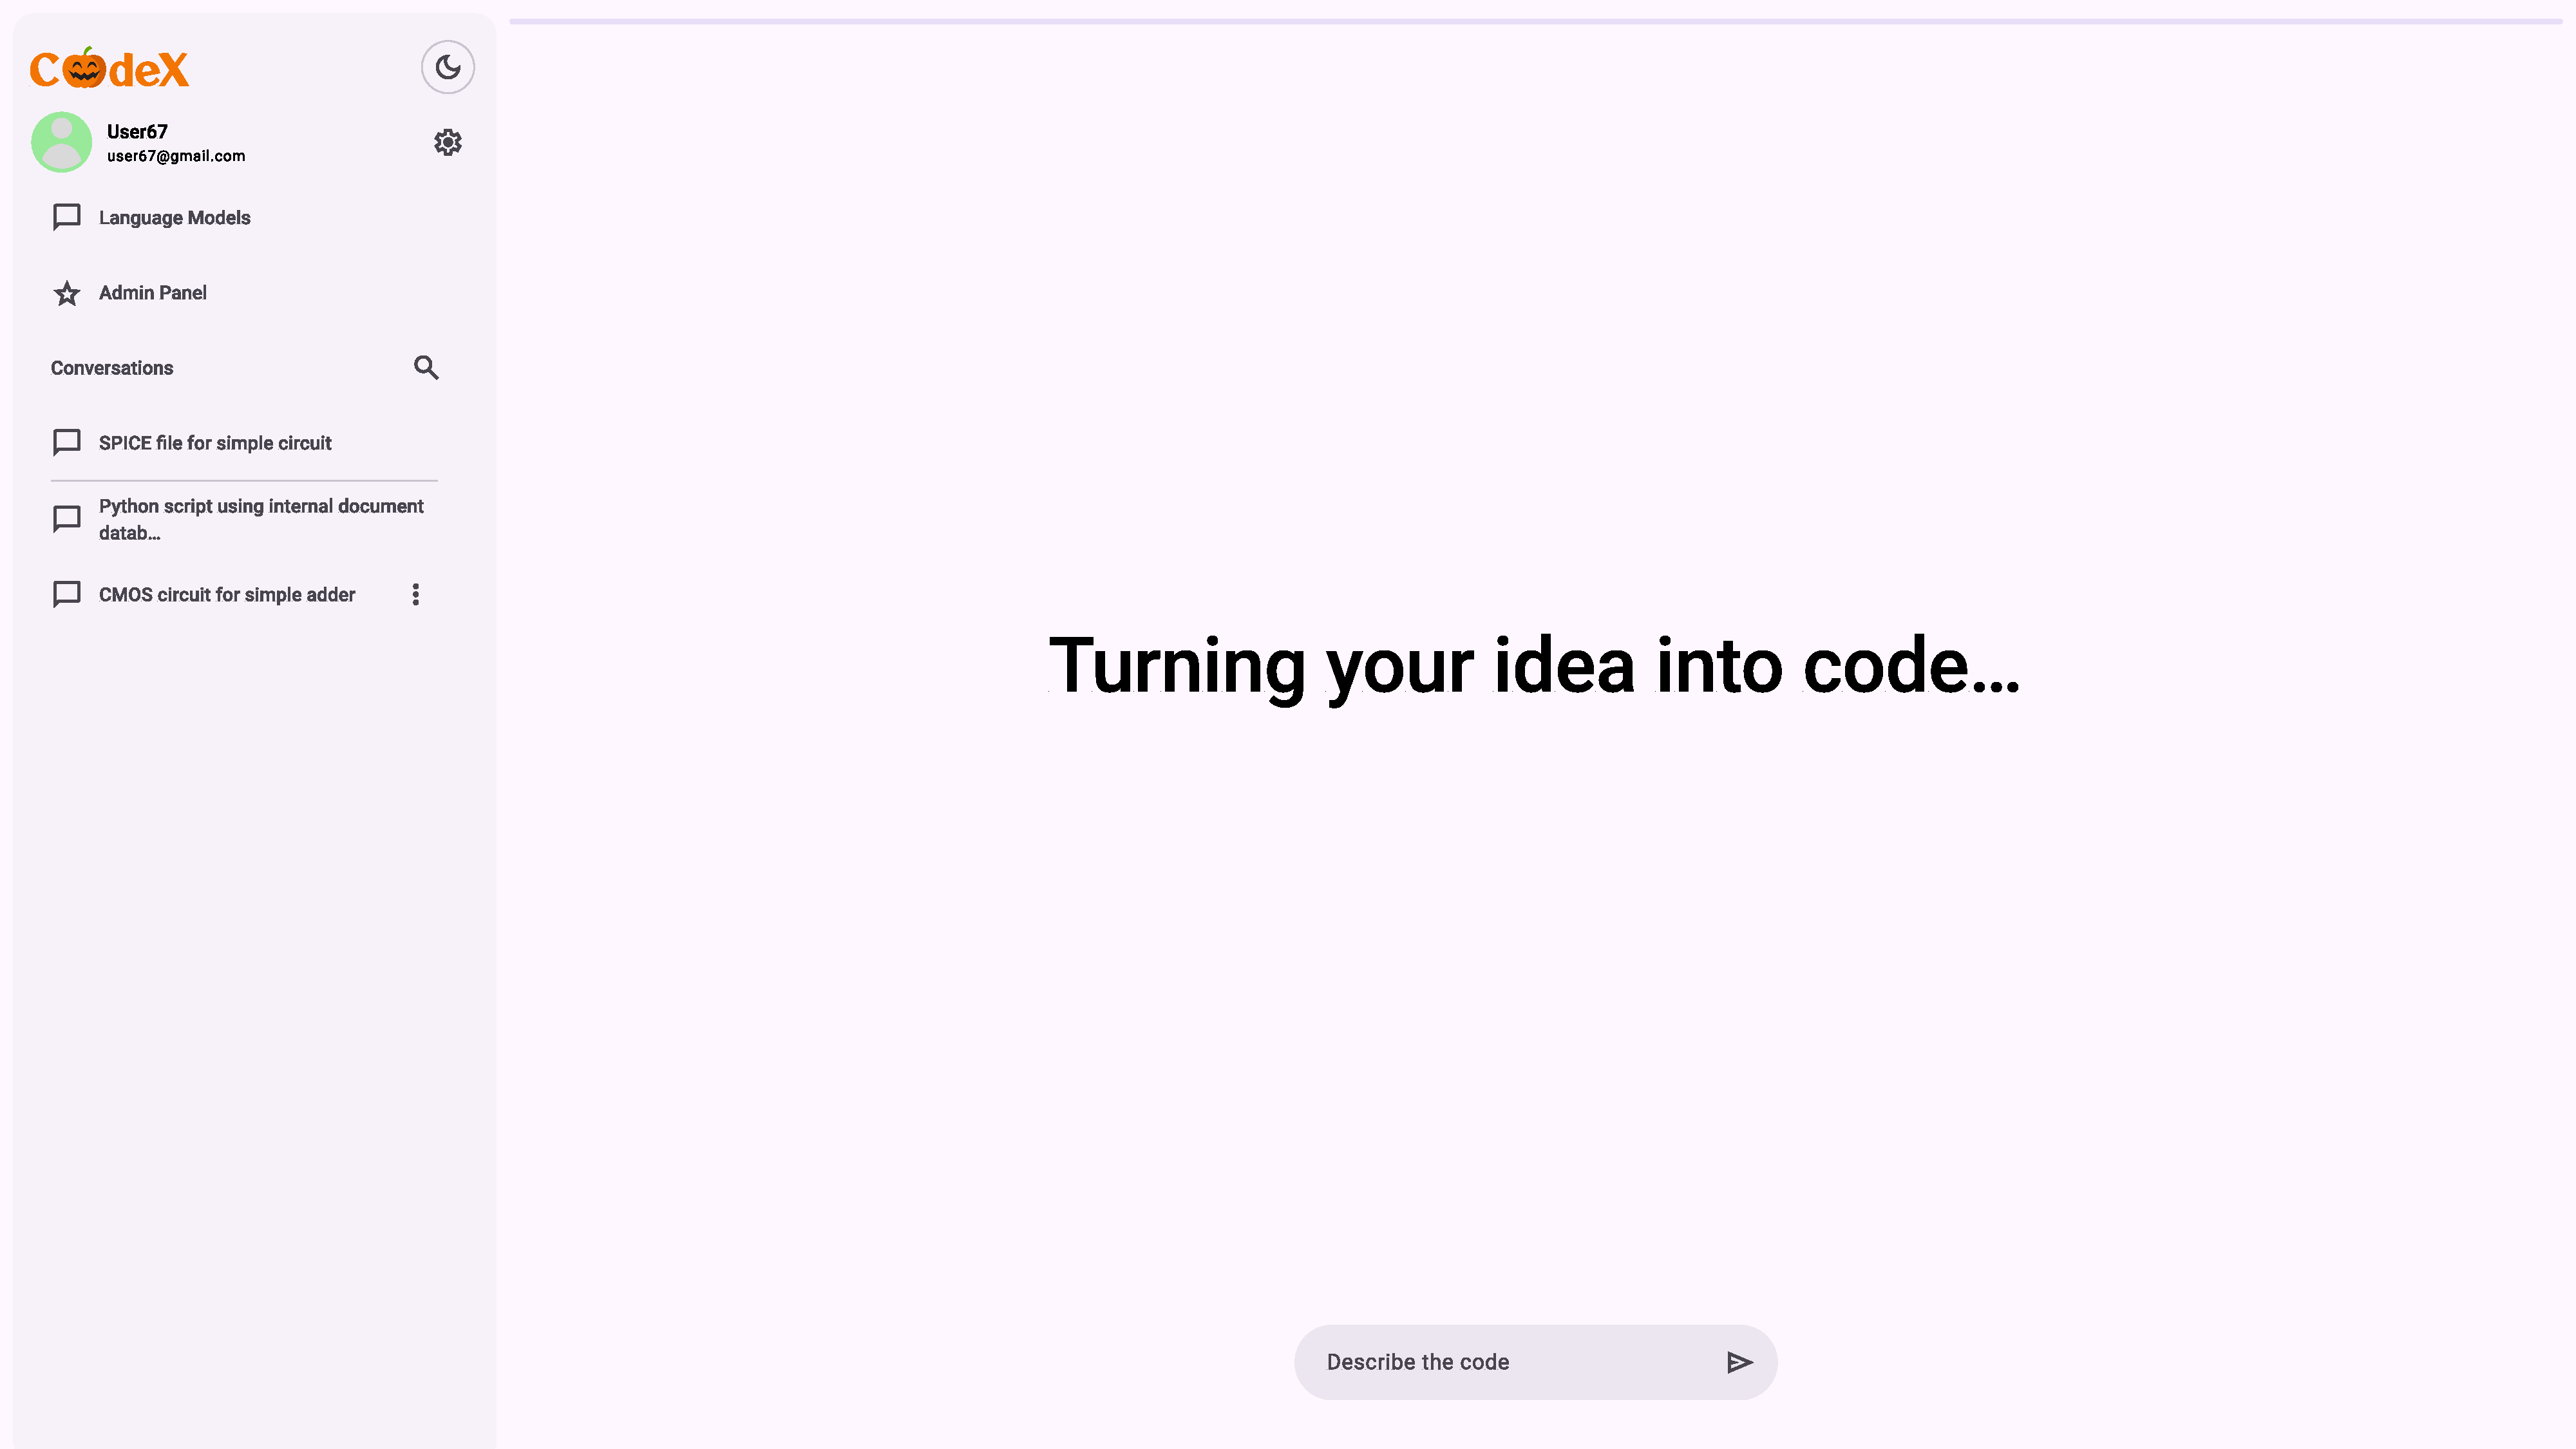
\includegraphics[width=\linewidth]{figures/ui/desktop/Conversation_Screen loading}
    \caption{\hyperref[abr:GUI]{GUI}: Conversation screen during request}
    \label{fig:ui_d_conversation_screen_loading}
\end{figure}
\begin{figure}
    \centering
    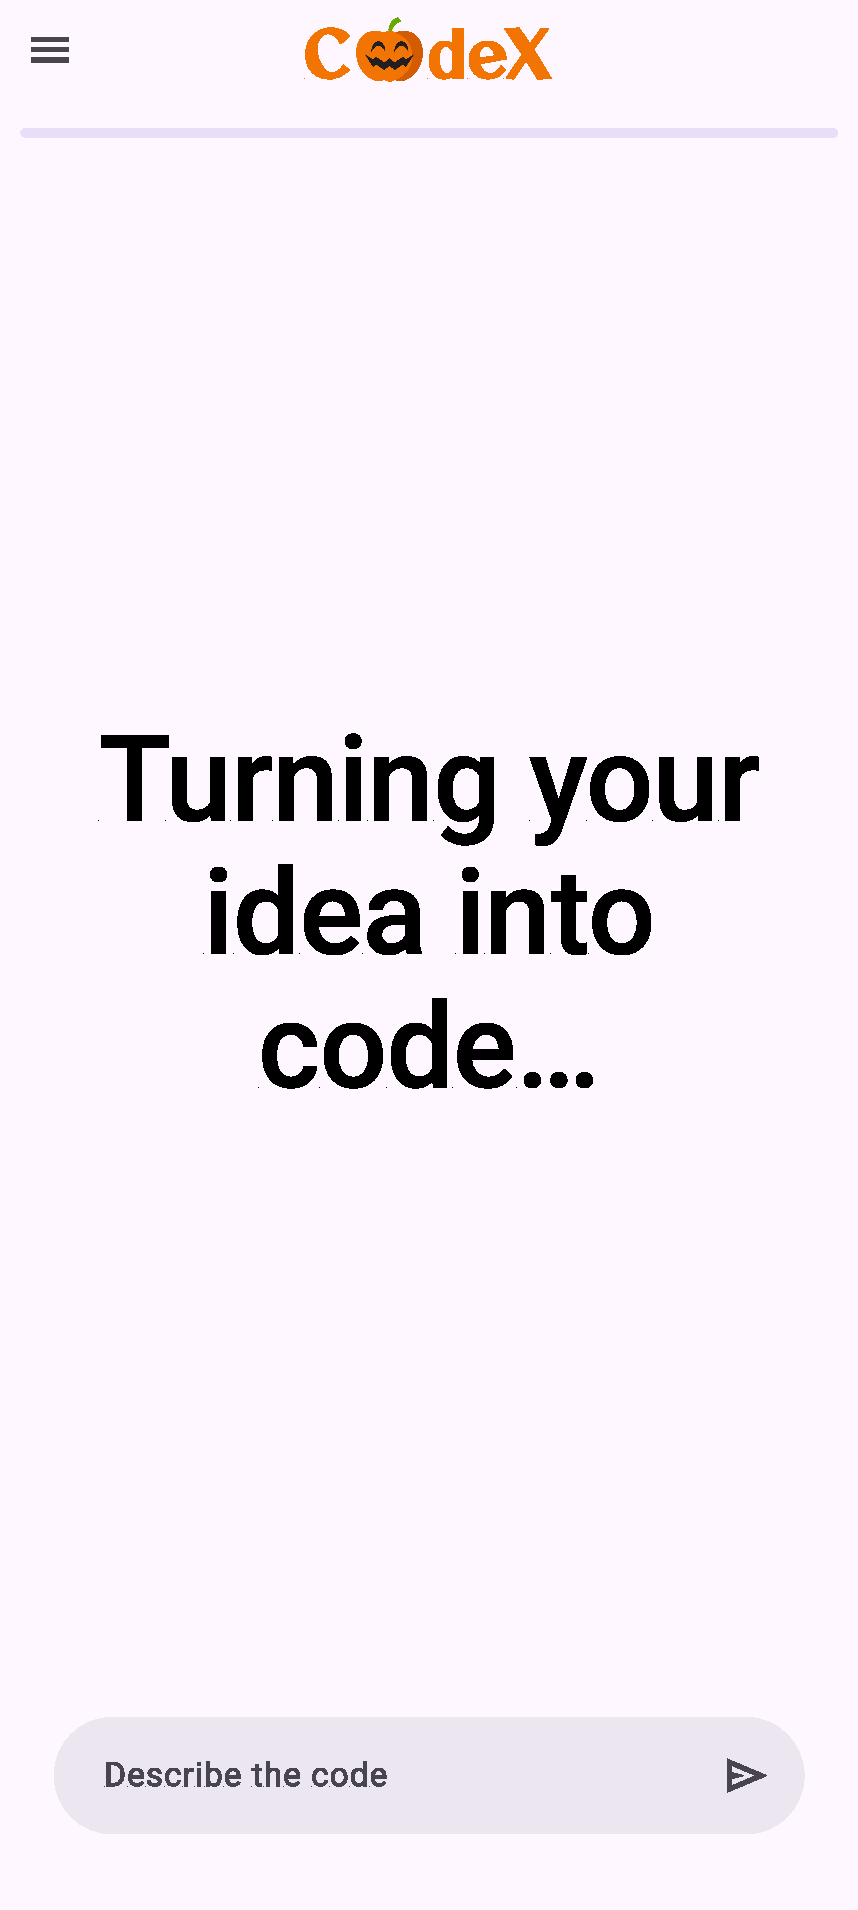
\includegraphics[width=5cm]{figures/ui/mobile/Conversation_Screen loading}
    \caption{\hyperref[abr:GUI]{GUI}: Conversation screen during request (mobile)}
    \label{fig:ui_m_conversation_screen_loading}
\end{figure}

\begin{figure}
    \centering
    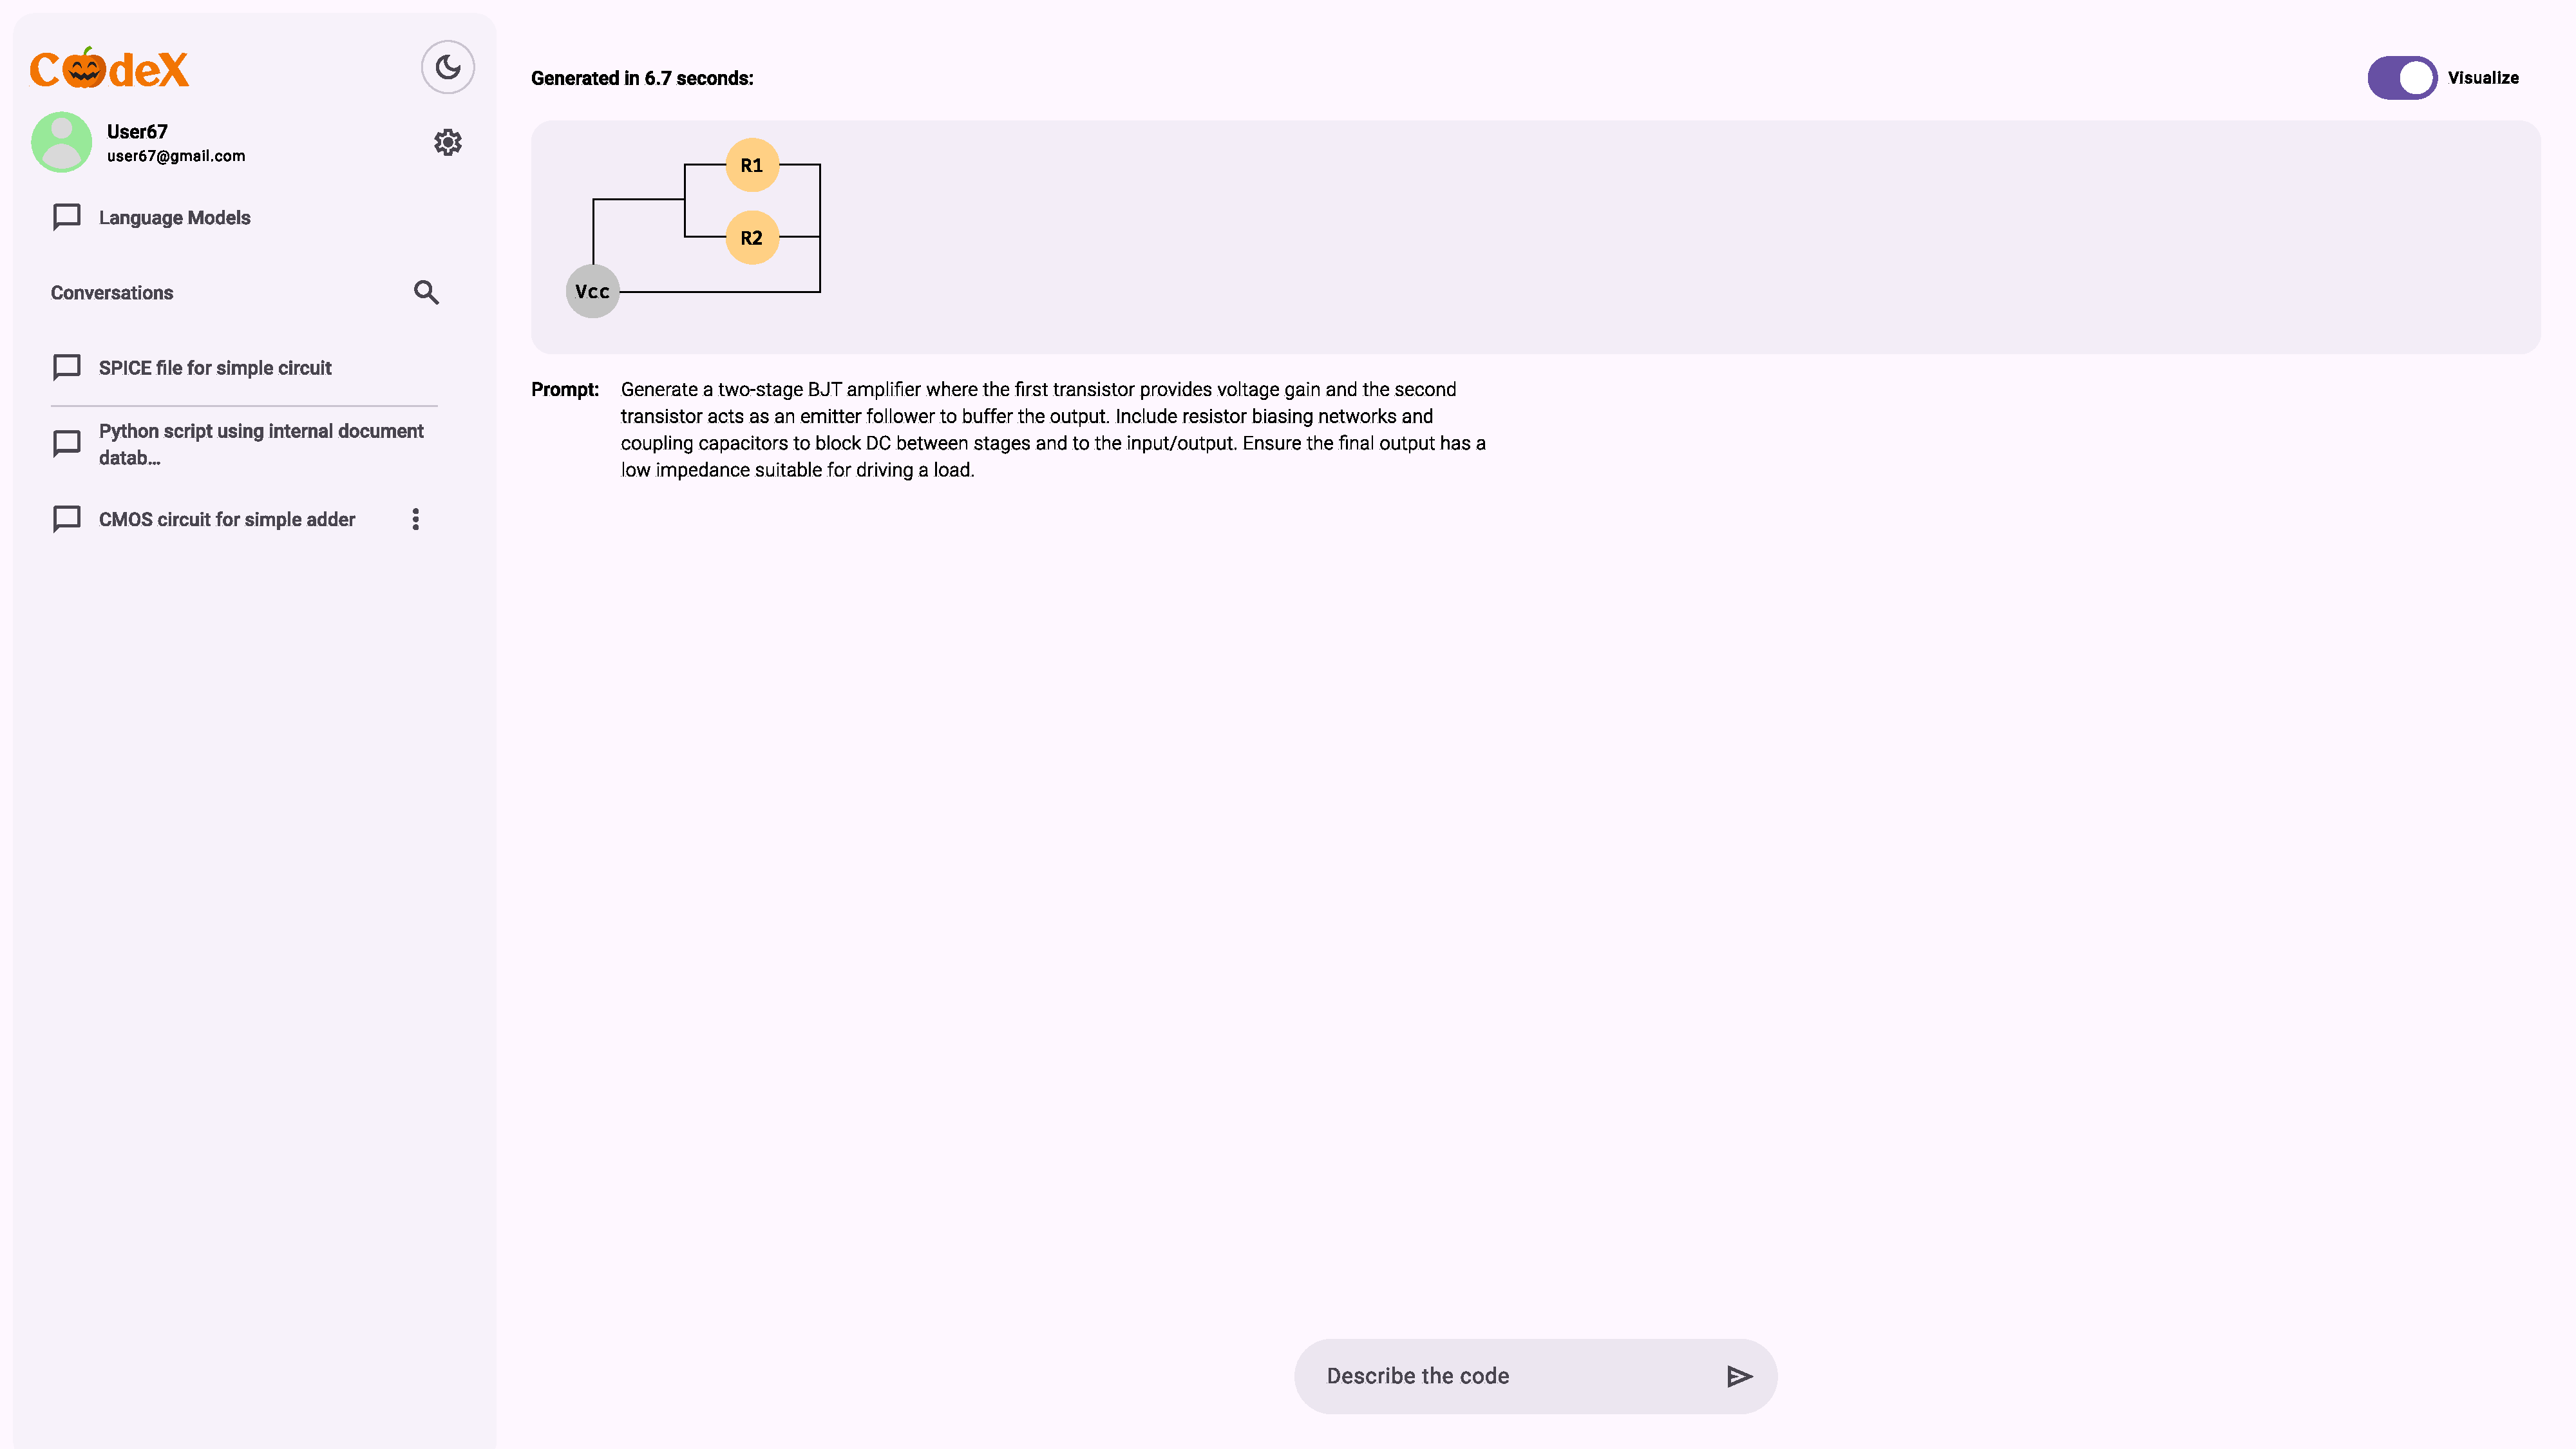
\includegraphics[width=\linewidth]{figures/ui/desktop/Conversation_Screen visualized}
    \caption{\hyperref[abr:GUI]{GUI}: Conversation screen after request with visualization}
    \label{fig:ui_d_conversation_screen_visualized}
\end{figure}
\begin{figure}
    \centering
    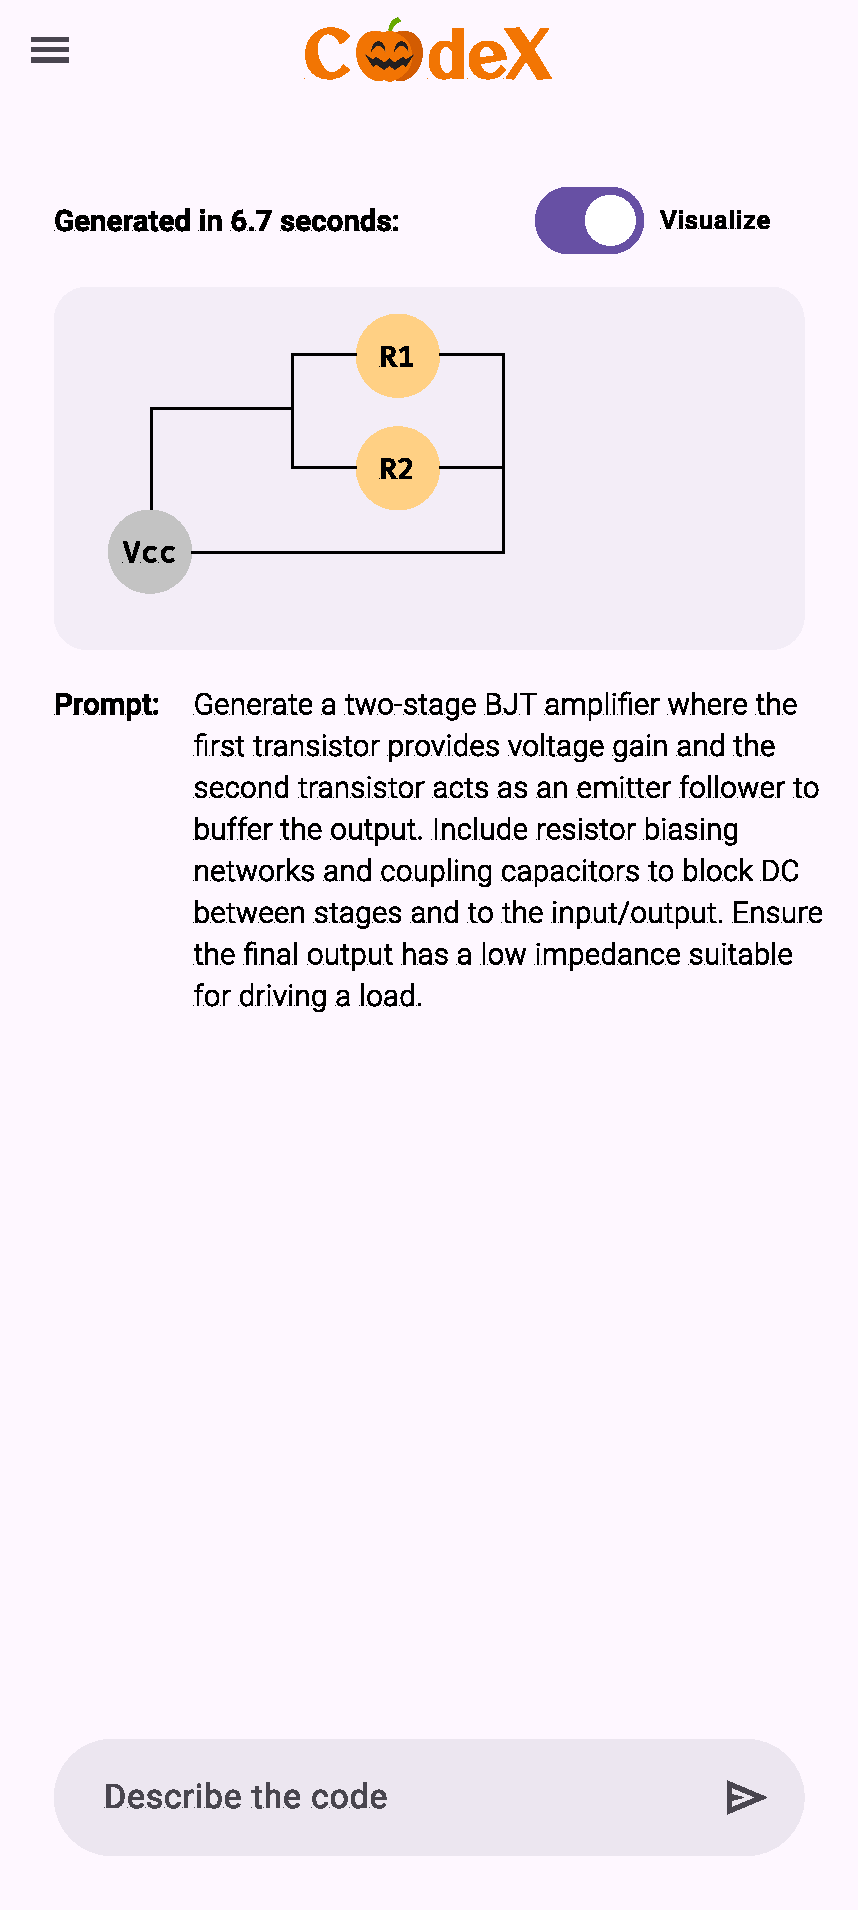
\includegraphics[width=5cm]{figures/ui/mobile/Conversation_Screen visualized}
    \caption{\hyperref[abr:GUI]{GUI}: Conversation screen after request with visualization (mobile)}
    \label{fig:ui_m_conversation_screen_visualized}
\end{figure}

\begin{figure}
    \centering
    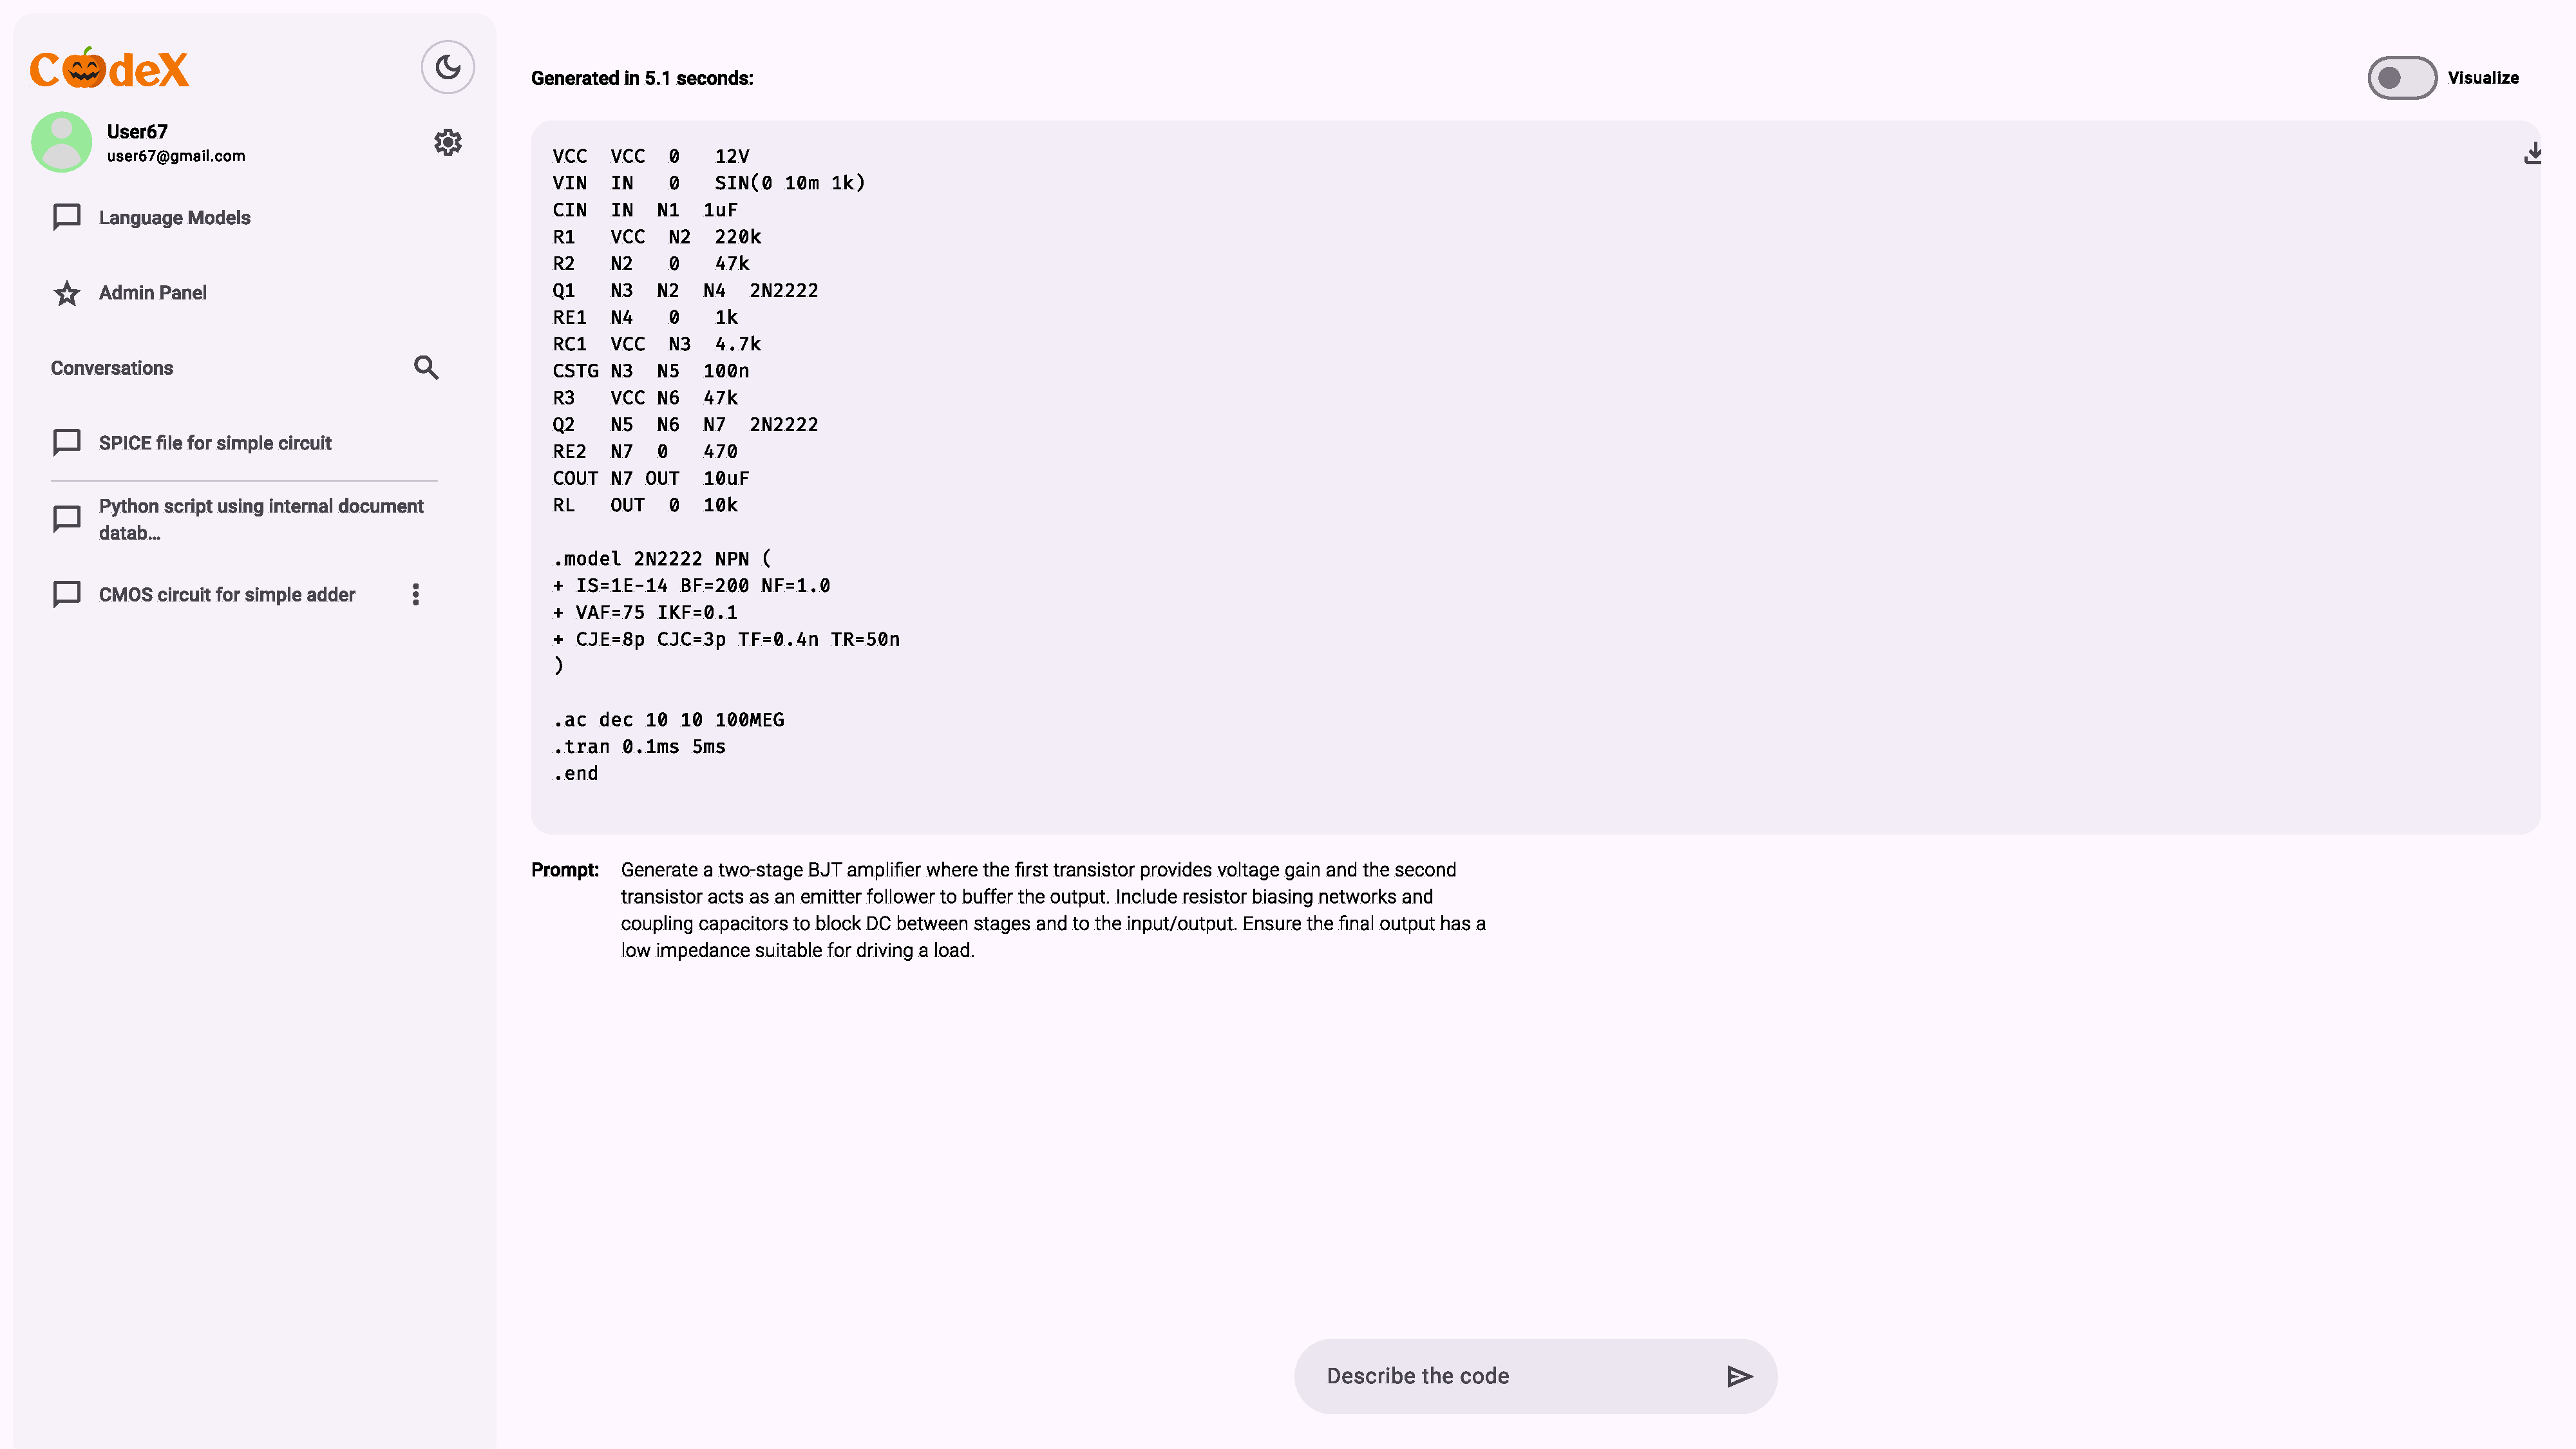
\includegraphics[width=\linewidth]{figures/ui/desktop/Conversation_Screen not-visualized}
    \caption{\hyperref[abr:GUI]{GUI}: Conversation screen after request without visualization}
    \label{fig:ui_d_conversation_screen_not_visualized}
\end{figure}
\begin{figure}
    \centering
    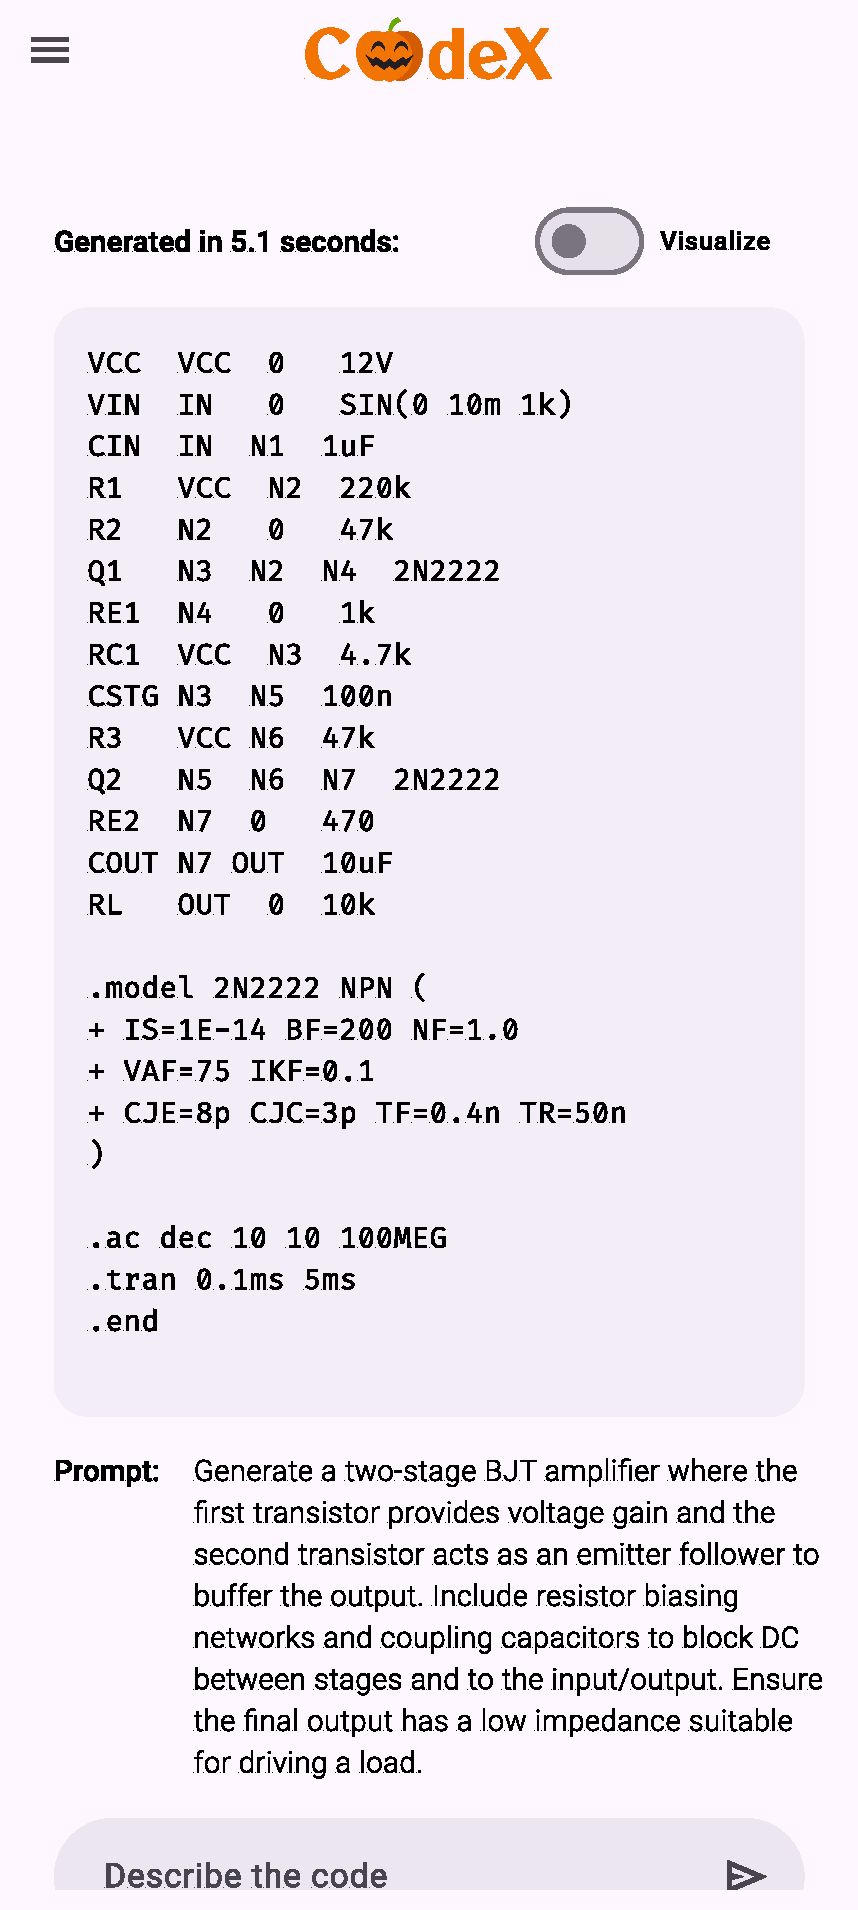
\includegraphics[width=5cm]{figures/ui/mobile/Conversation_Screen not-visualized}
    \caption{\hyperref[abr:GUI]{GUI}: Conversation screen after request without visualization (mobile)}
    \label{fig:ui_m_conversation_screen_not_visualized}
\end{figure}

\subsection{Admin Panel}
The admin panel (\ref{fig:ui-d-admin-panel}/\ref{fig:ui-m-admin-panel}) is where admins can view analytics and update quota settings.
\begin{figure}
    \centering
    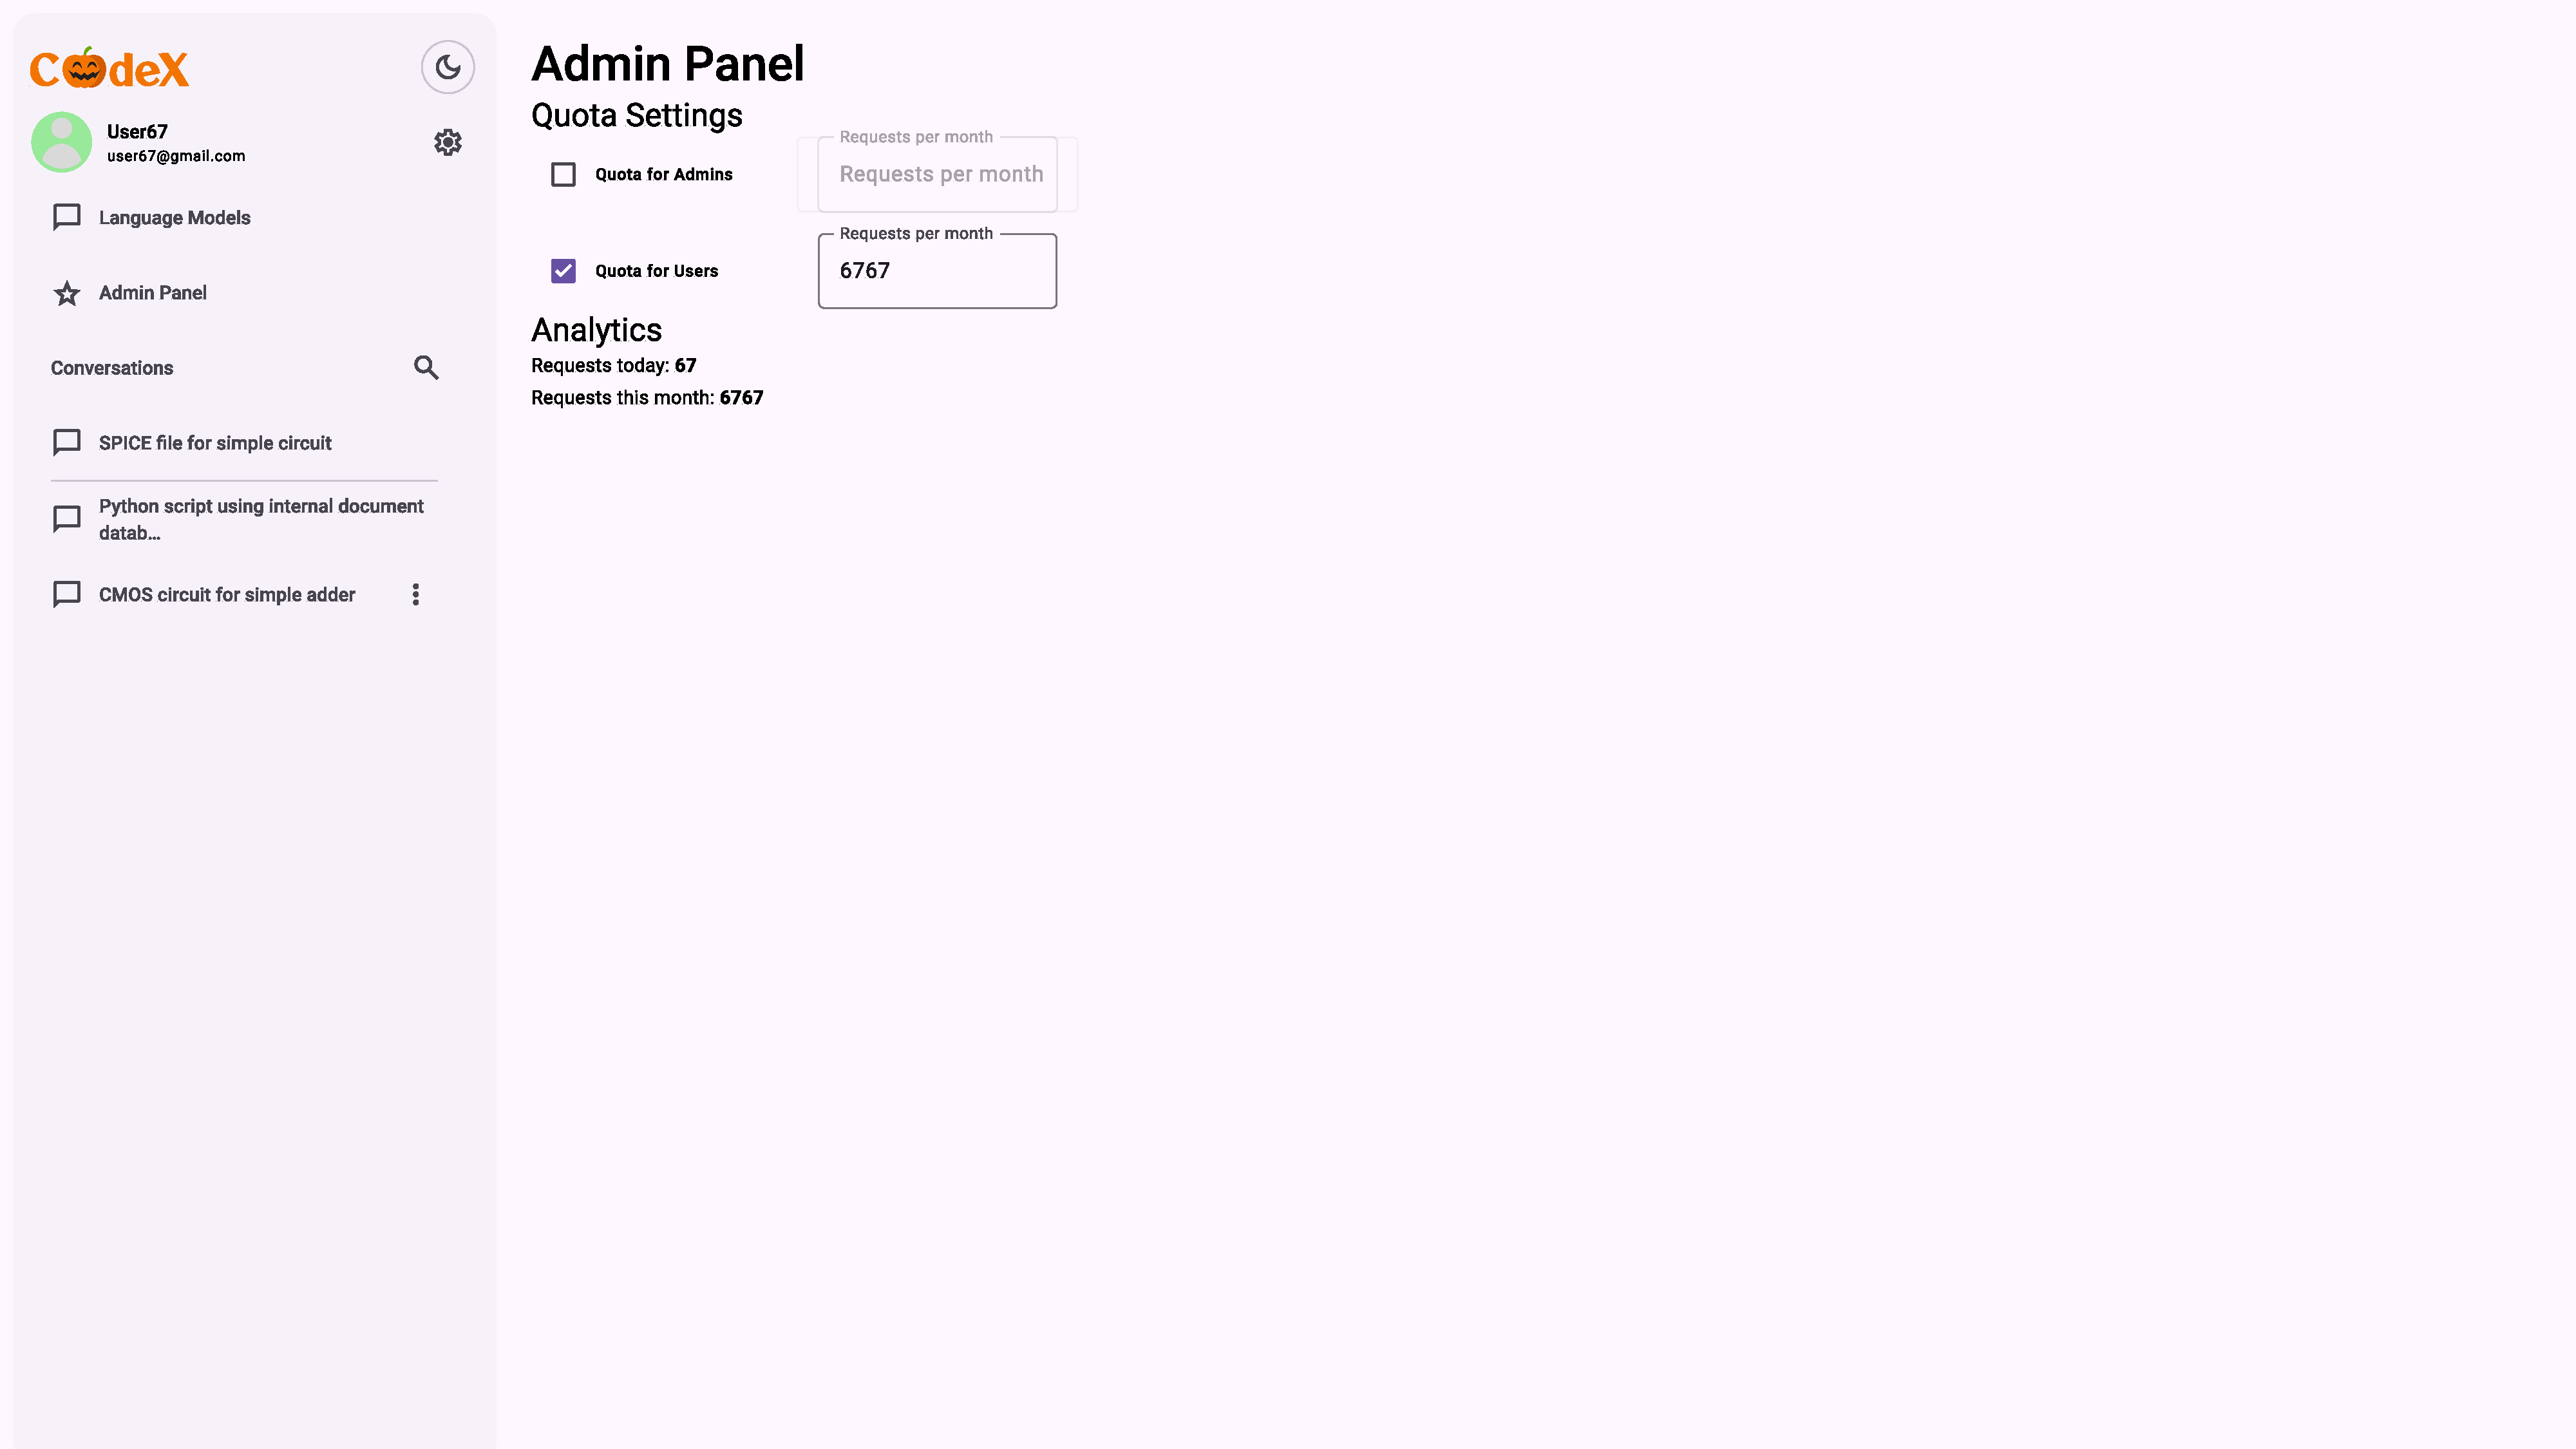
\includegraphics[width=\linewidth]{figures/ui/desktop/Admin_Panel_Screen}
    \caption{\hyperref[abr:GUI]{GUI}: Admin panel}
    \label{fig:ui-d-admin-panel}
\end{figure}
\begin{figure}
    \centering
    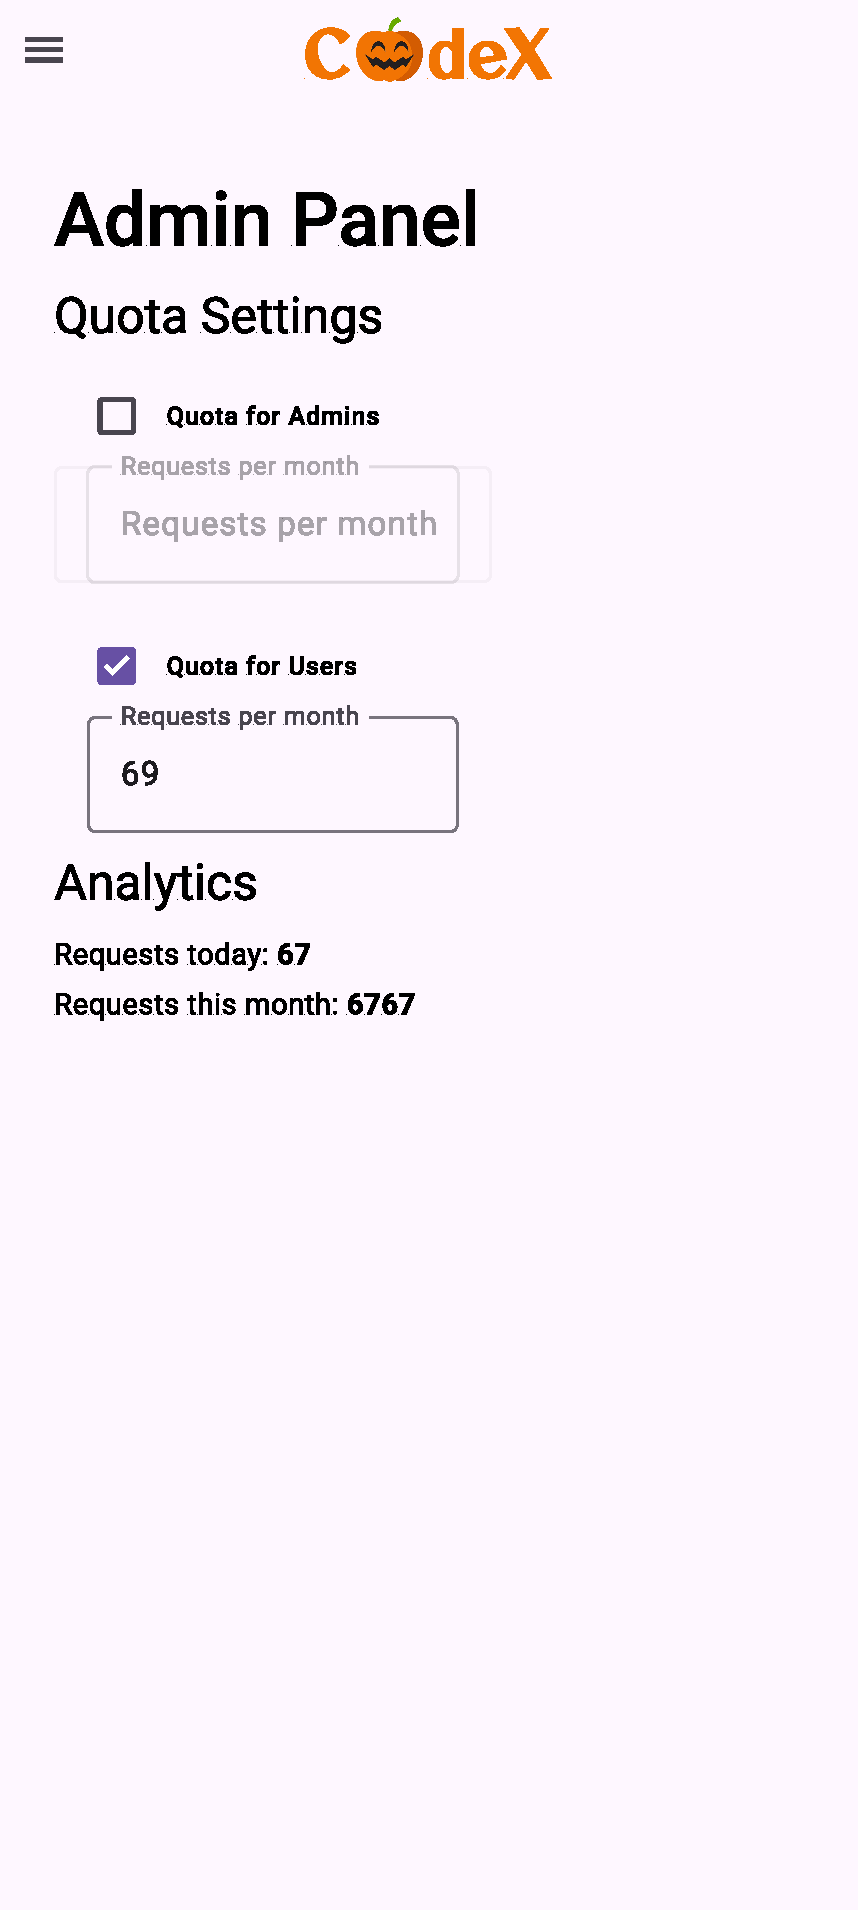
\includegraphics[width=5cm]{figures/ui/mobile/Admin_Panel_Screen}
    \caption{\hyperref[abr:GUI]{GUI}: Admin panel (mobile)}
    \label{fig:ui-m-admin-panel}
\end{figure}

\subsection{Settings}
The settings screen (\ref{fig:ui-d-settings}/\ref{fig:ui-m-settings}) is where the user can add, delete and update LLM-configurations.
\begin{figure}
    \centering
    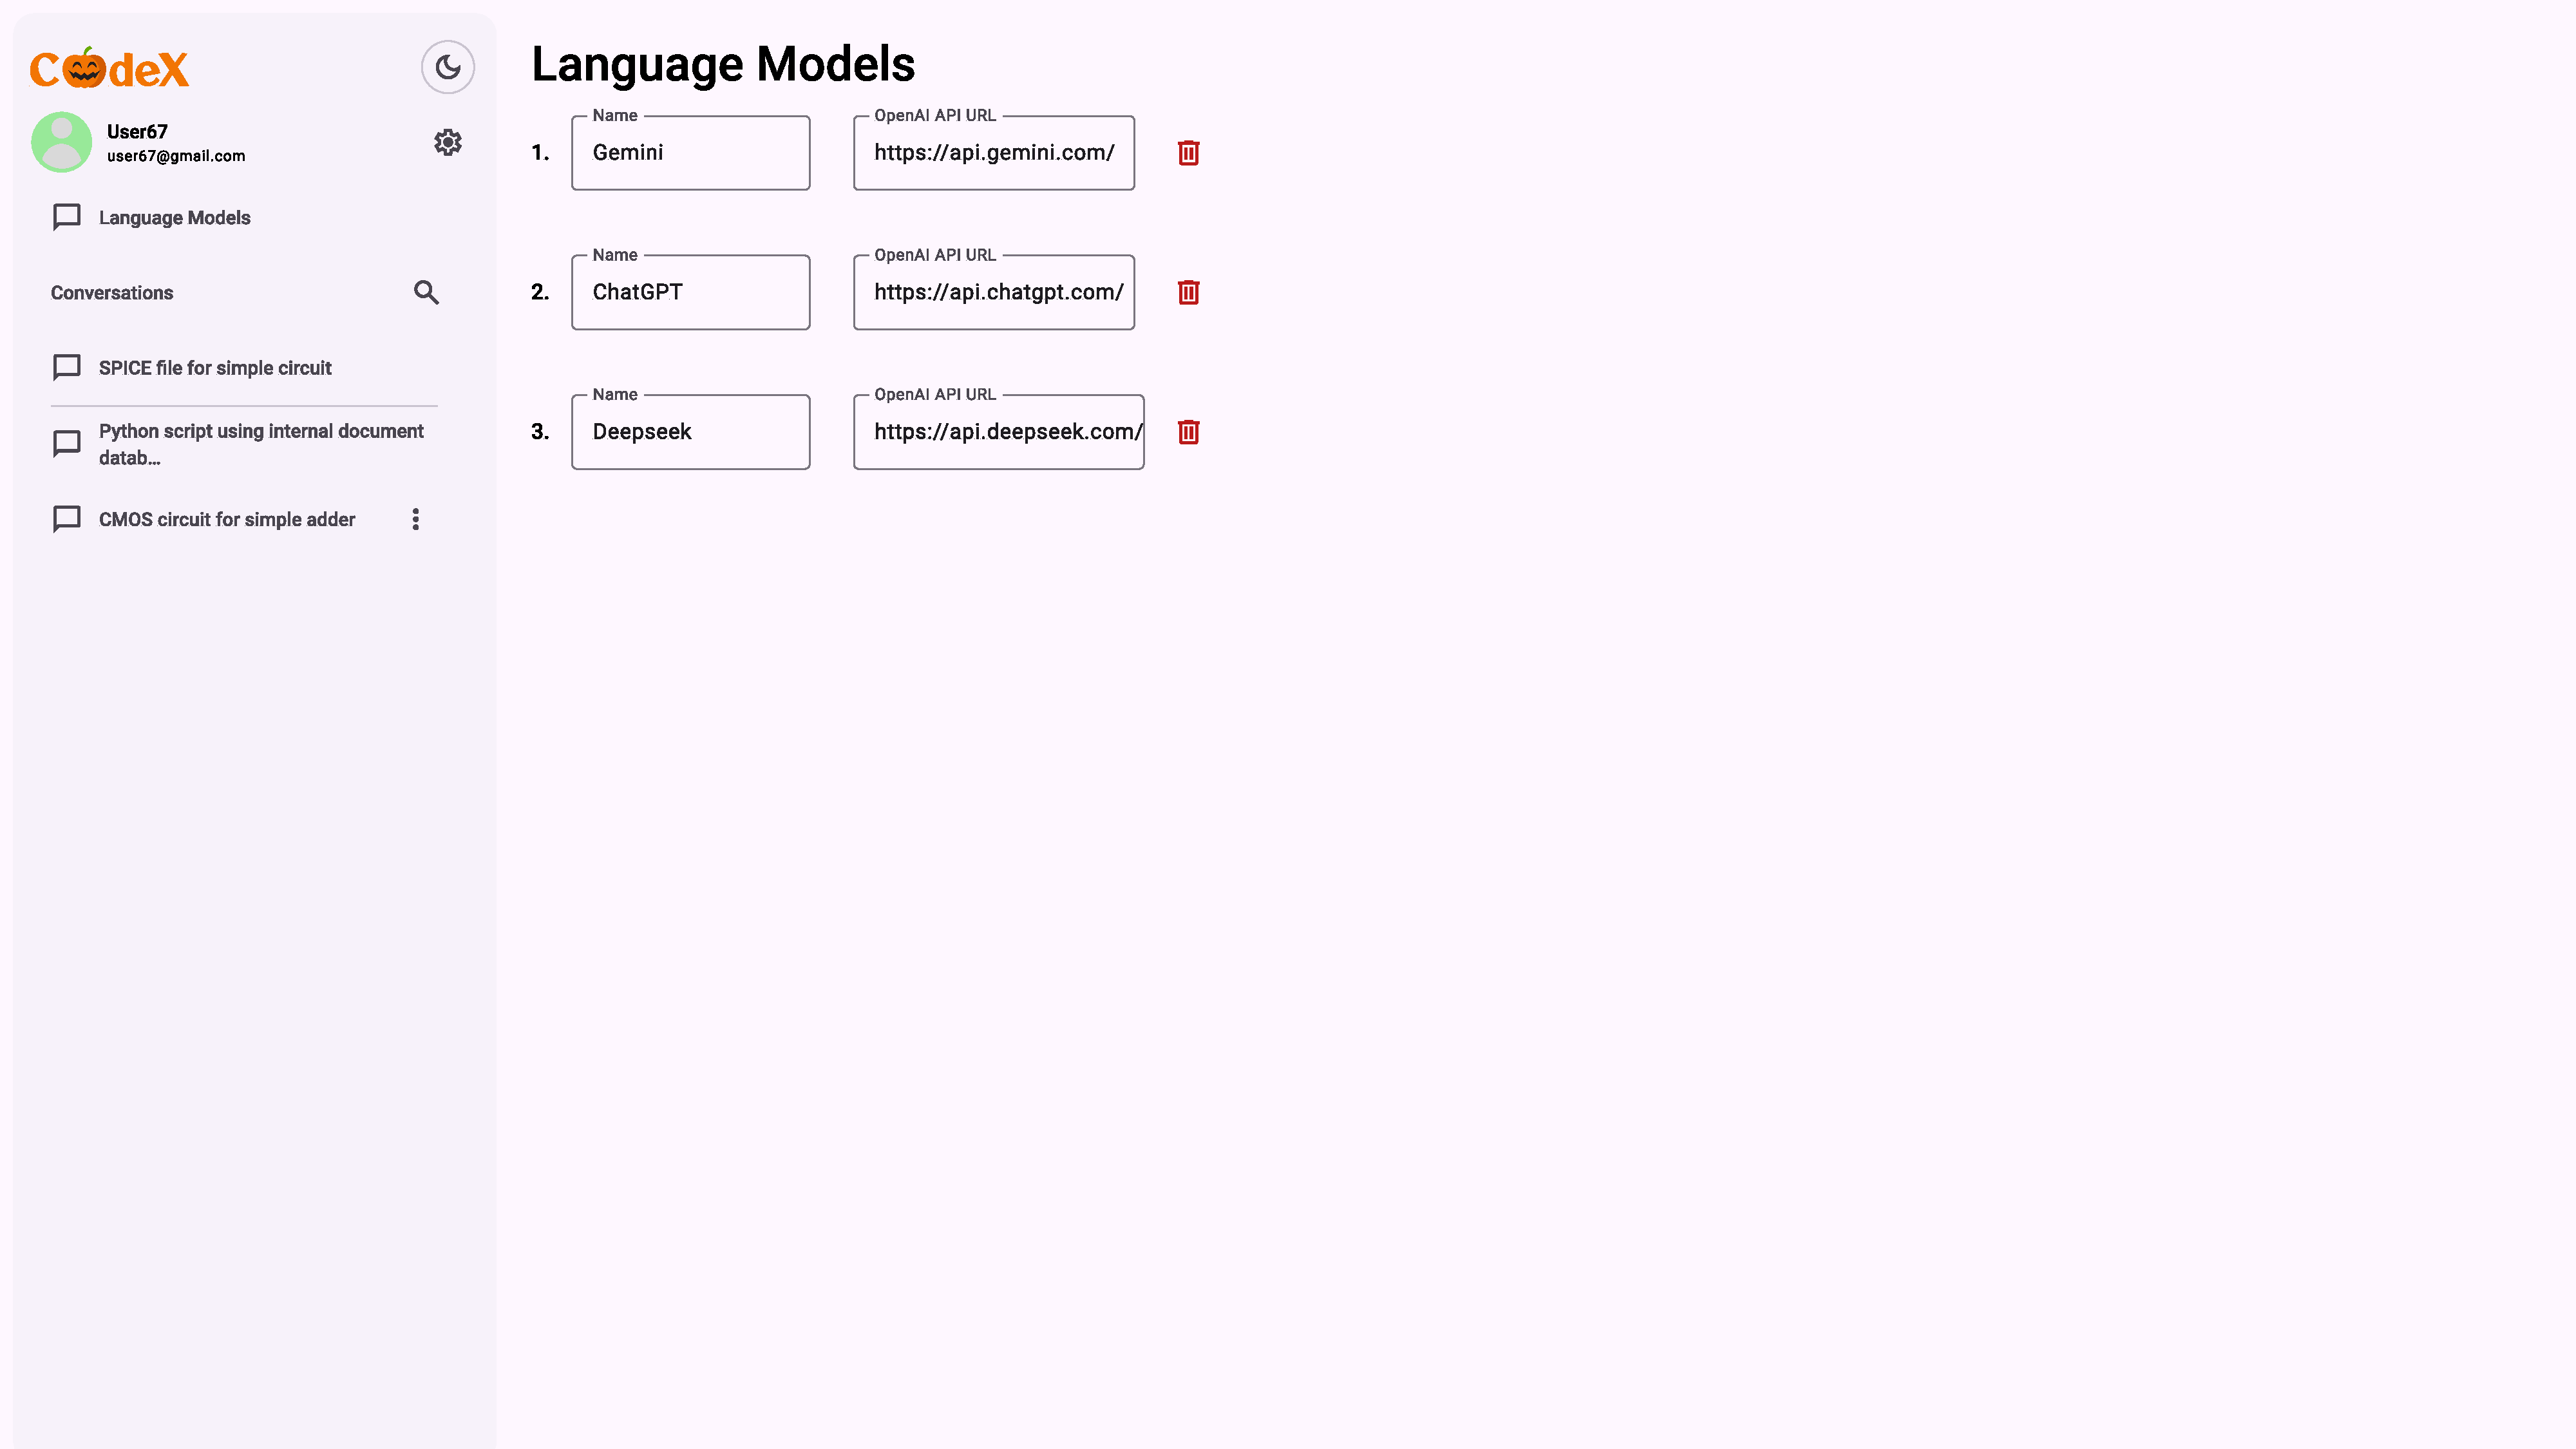
\includegraphics[width=\linewidth]{figures/ui/desktop/Settings_Screen}
    \caption{\hyperref[abr:GUI]{GUI}: Admin panel}
    \label{fig:ui-d-settings}
\end{figure}
\begin{figure}
    \centering
    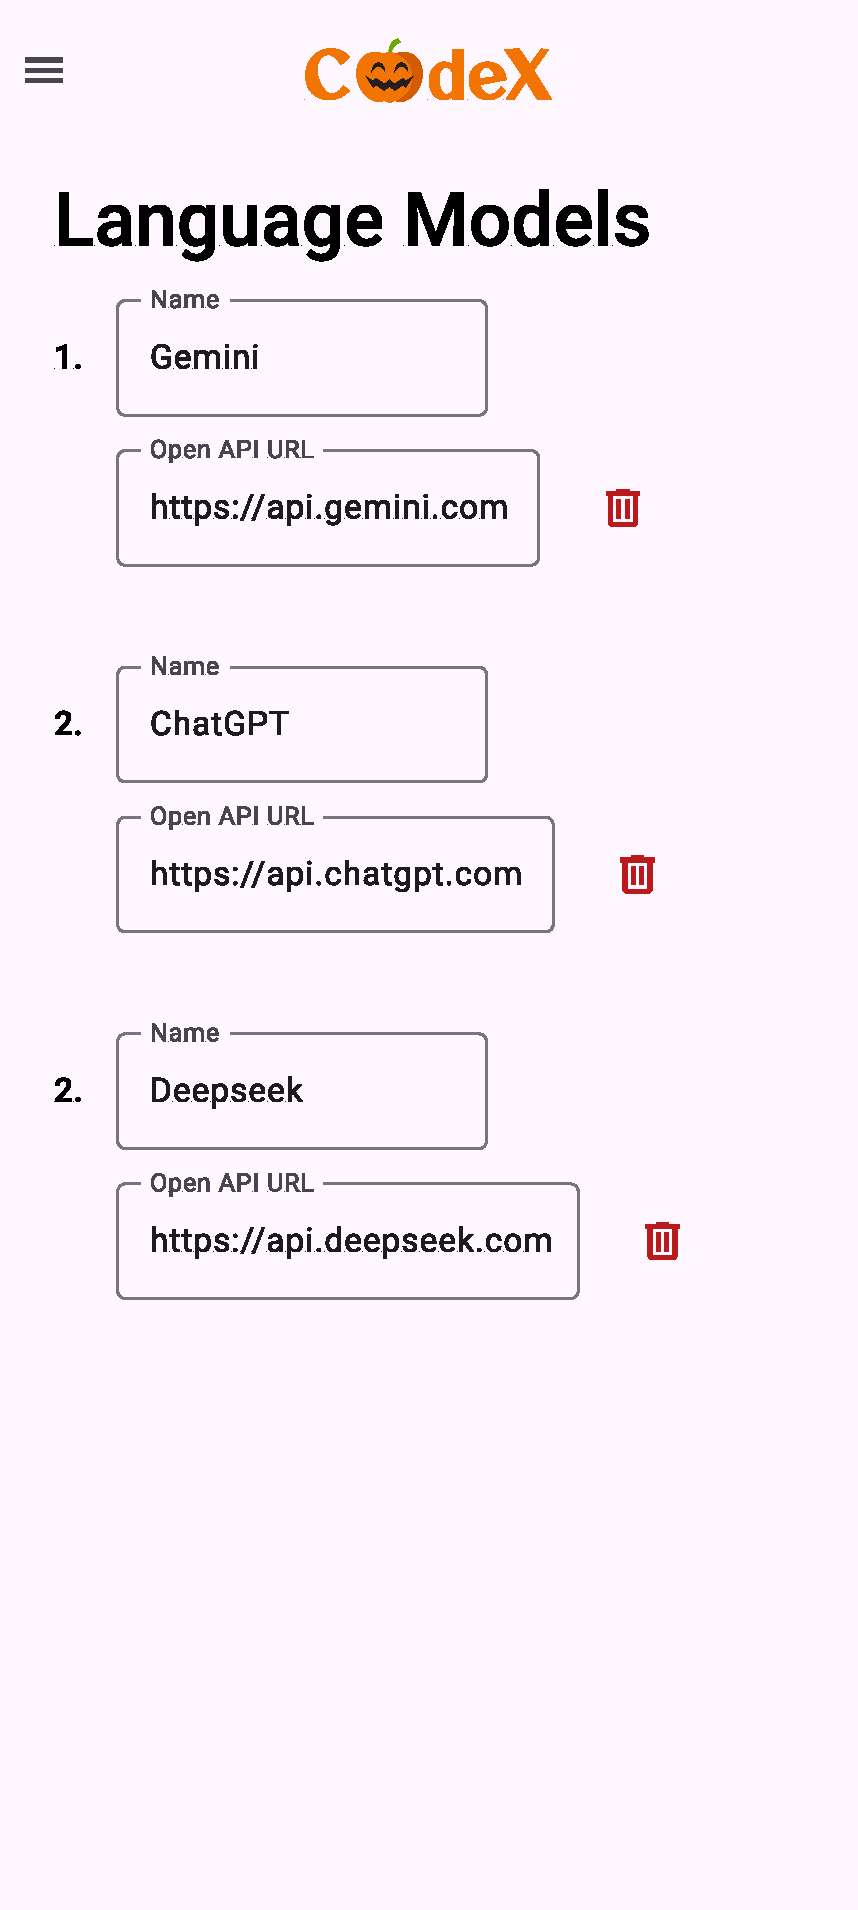
\includegraphics[width=5cm]{figures/ui/mobile/Settings_Screen}
    \caption{\hyperref[abr:GUI]{GUI}: Admin panel (mobile)}
    \label{fig:ui-m-settings}
\end{figure}

\subsection{Log-in}
The log-in screen (\ref{fig:ui-d-login}/\ref{fig:ui-m-login}) allows an unauthenticated user to login by entering the credentials to an account.
Users can also opt to reset their password, go to the signup screen or continue with an \textit{\hyperref[def:oauth]{OAuth} provider}.
\begin{figure}
    \centering
    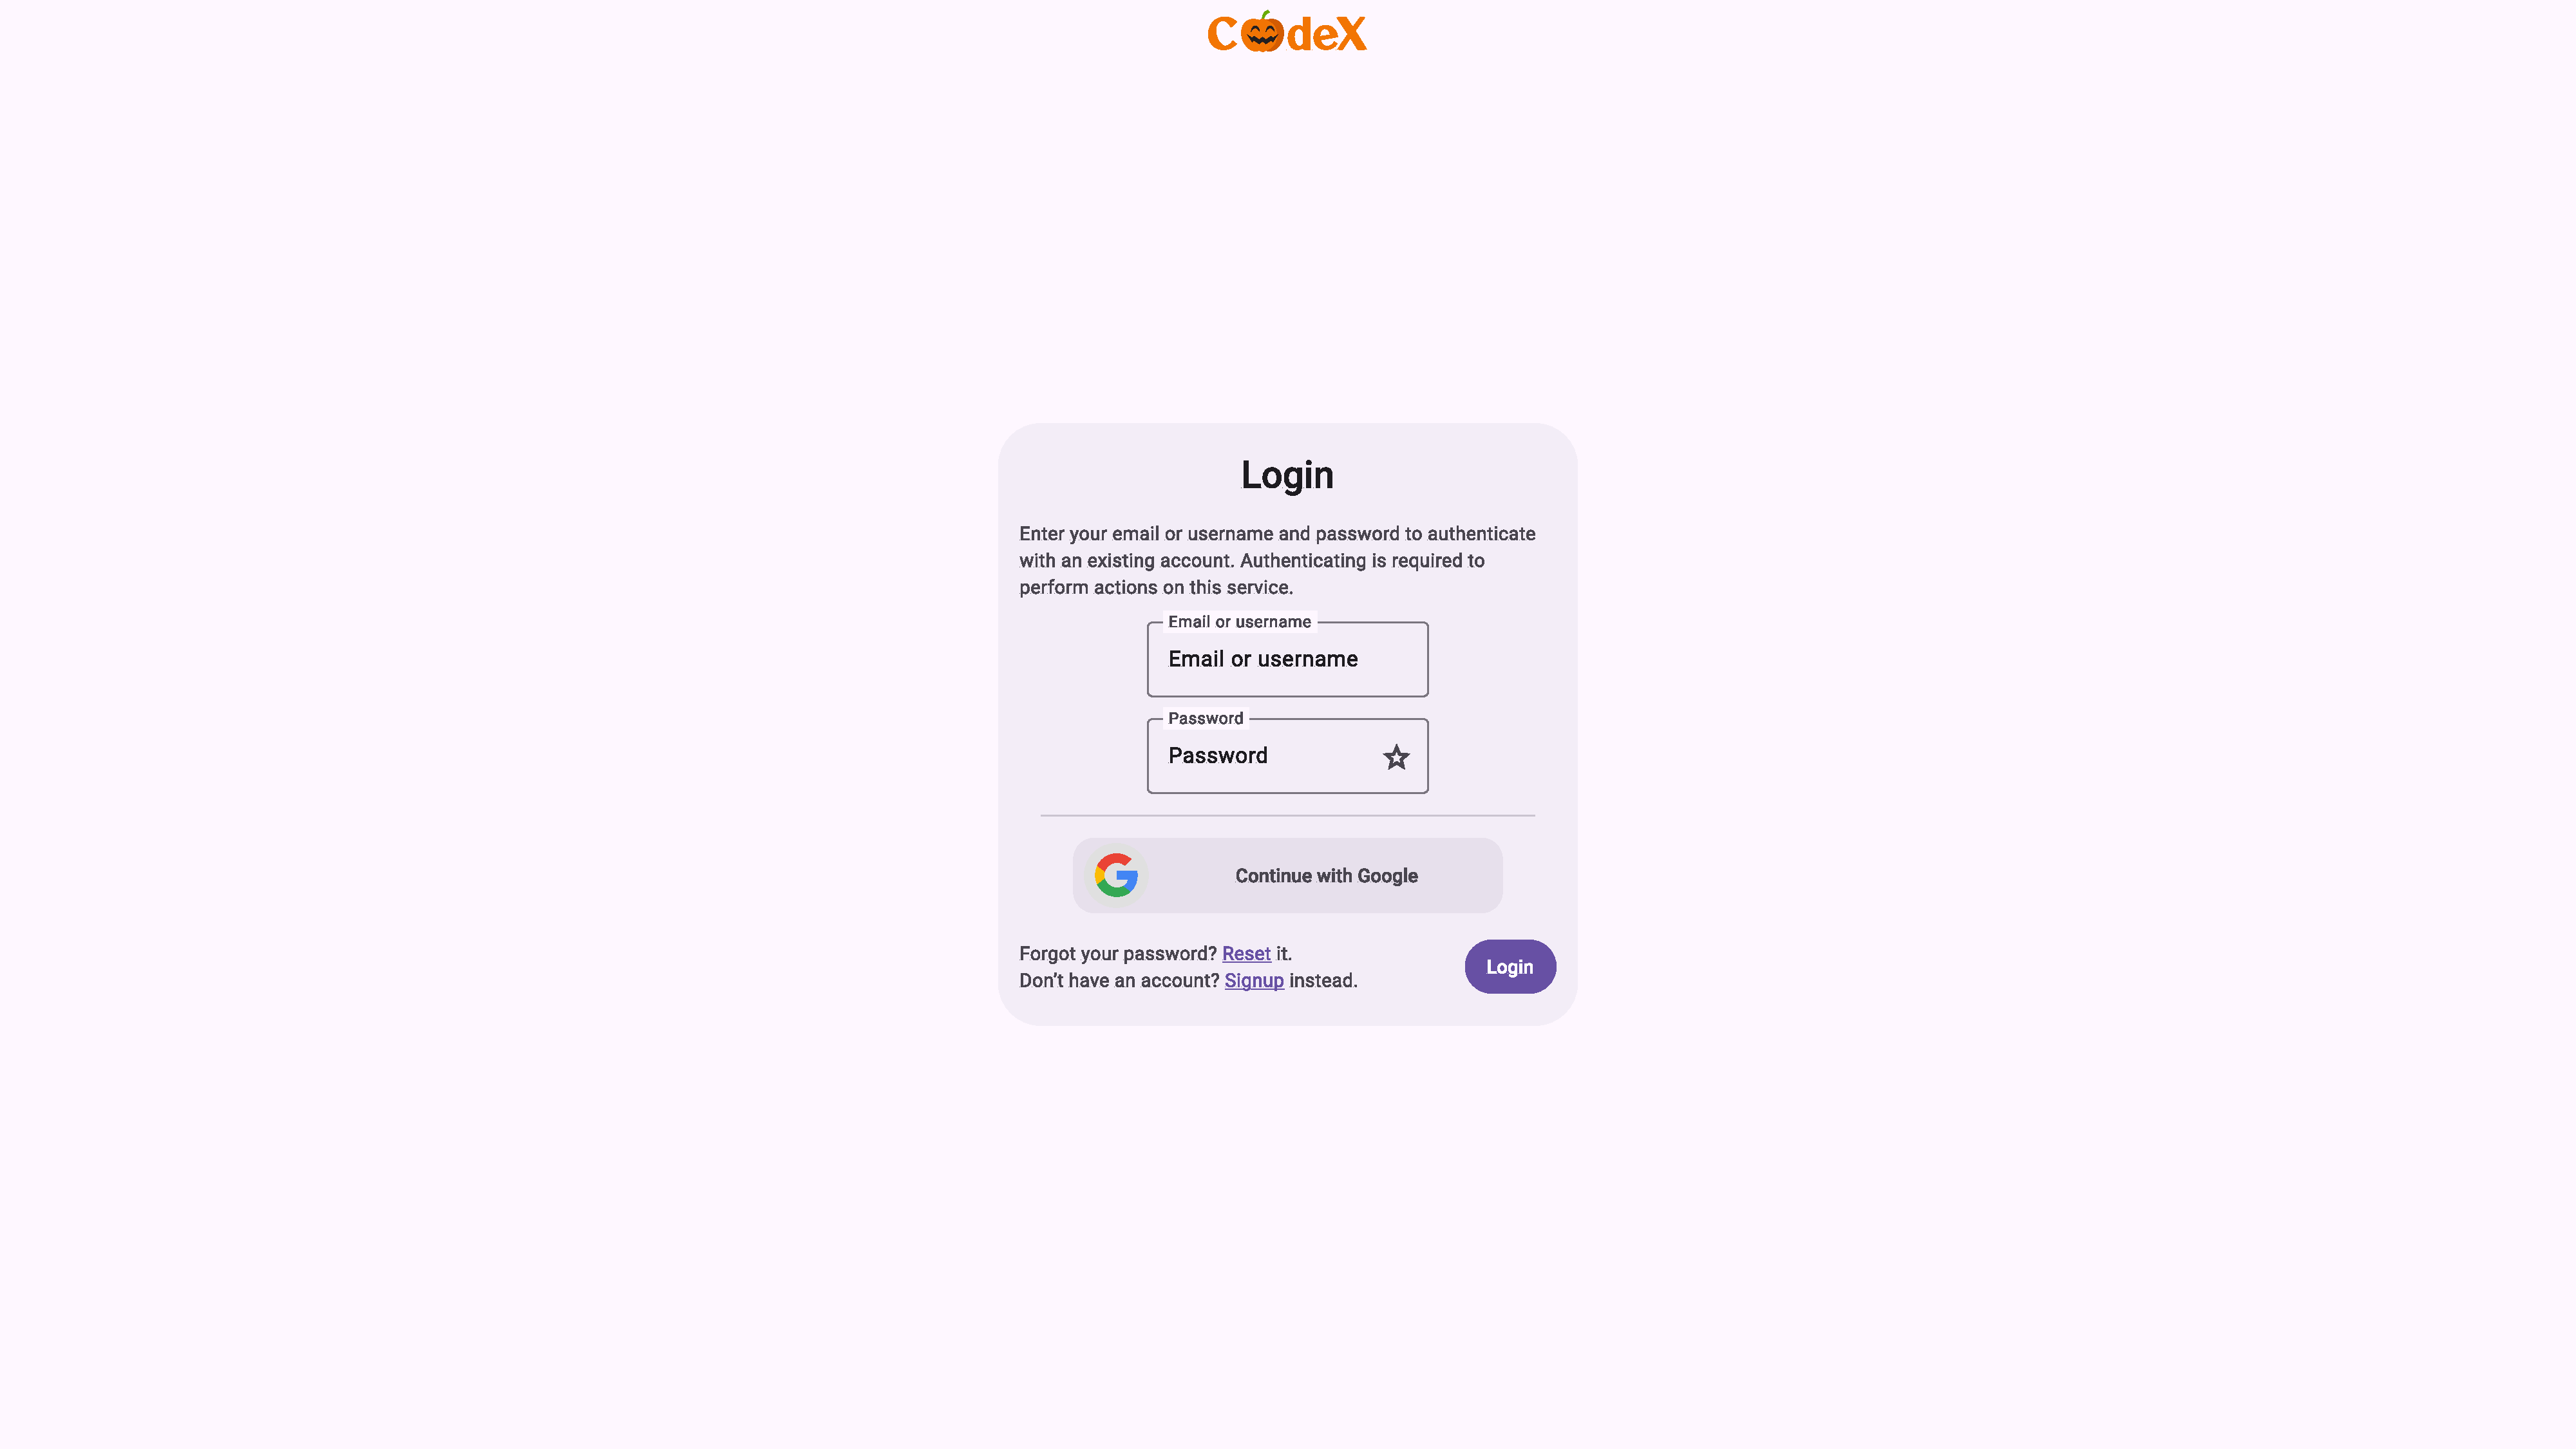
\includegraphics[width=\linewidth]{figures/ui/desktop/Login_Screen}
    \caption{\hyperref[abr:GUI]{GUI}: Log-in screen}
    \label{fig:ui-d-login}
\end{figure}
\begin{figure}
    \centering
    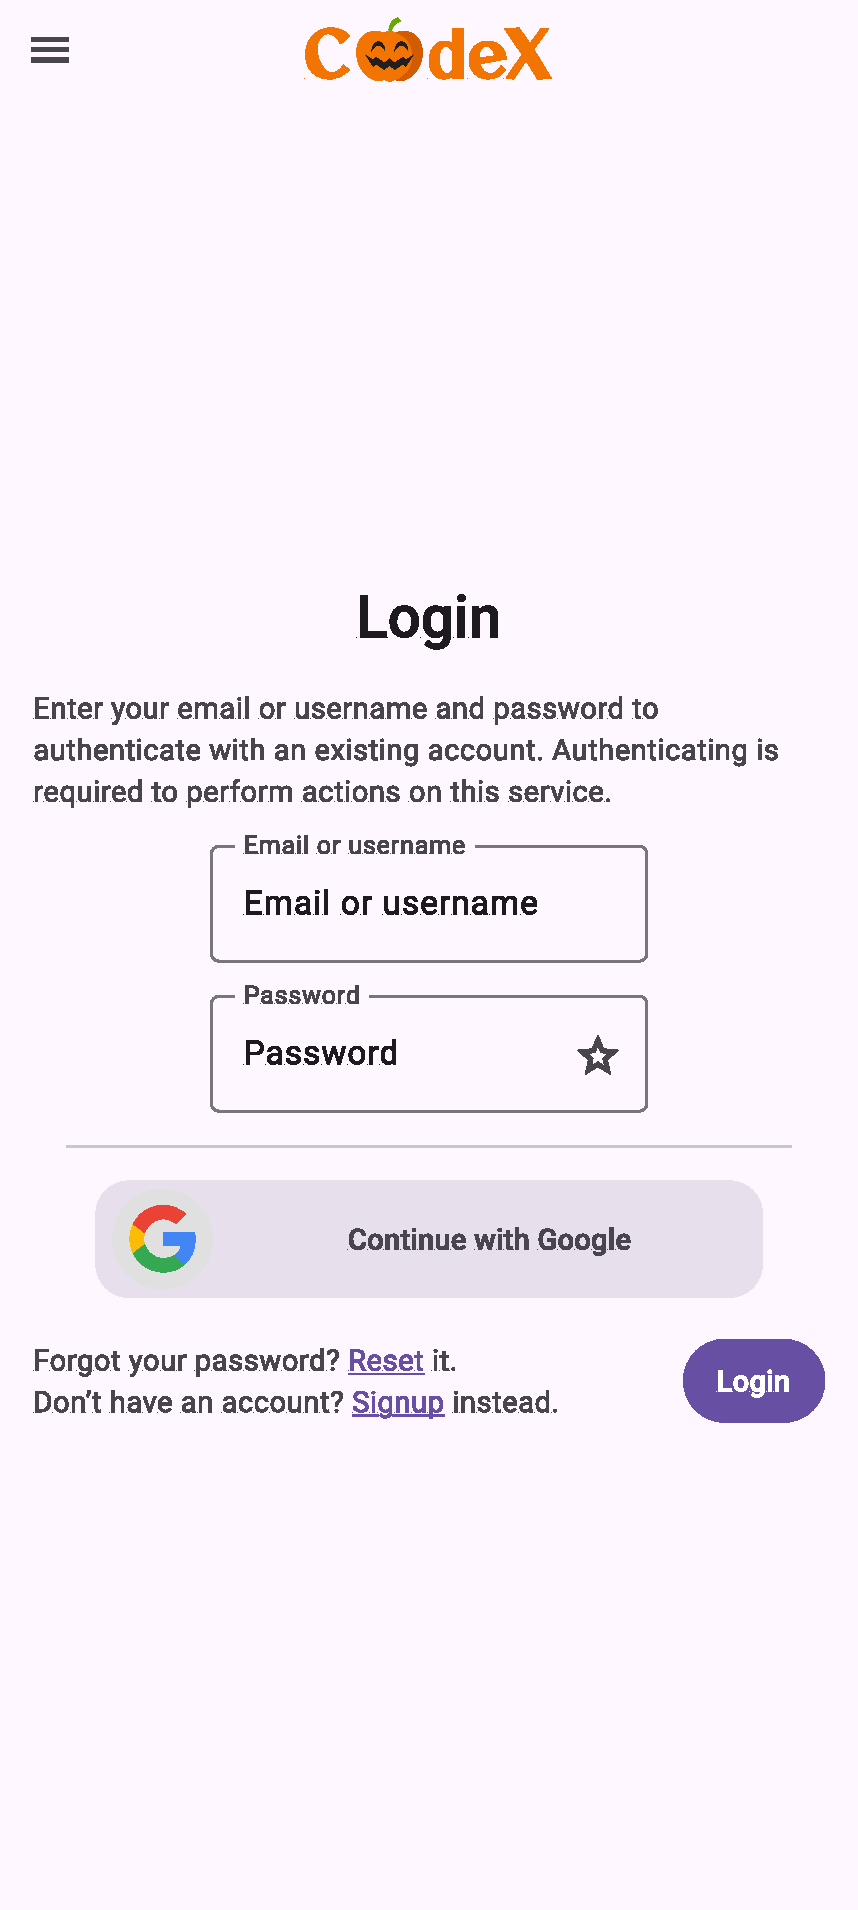
\includegraphics[width=5cm]{figures/ui/mobile/Login_Screen}
    \caption{\hyperref[abr:GUI]{GUI}: Log-in screen (mobile)}
    \label{fig:ui-m-login}
\end{figure}

\subsection{Request password reset}
The request password reset allows users that lost access to their account to request a password reset.
Users can enter the email of their account (\ref{fig:ui-d-request-reset-password-initial}/\ref{fig:ui-m-request-reset-password-initial}) and after confirming, an informative message is shown (\ref{fig:ui-d-request-reset-password-requested}/\ref{fig:ui-m-request-reset-password-requested}).
\begin{figure}
    \centering
    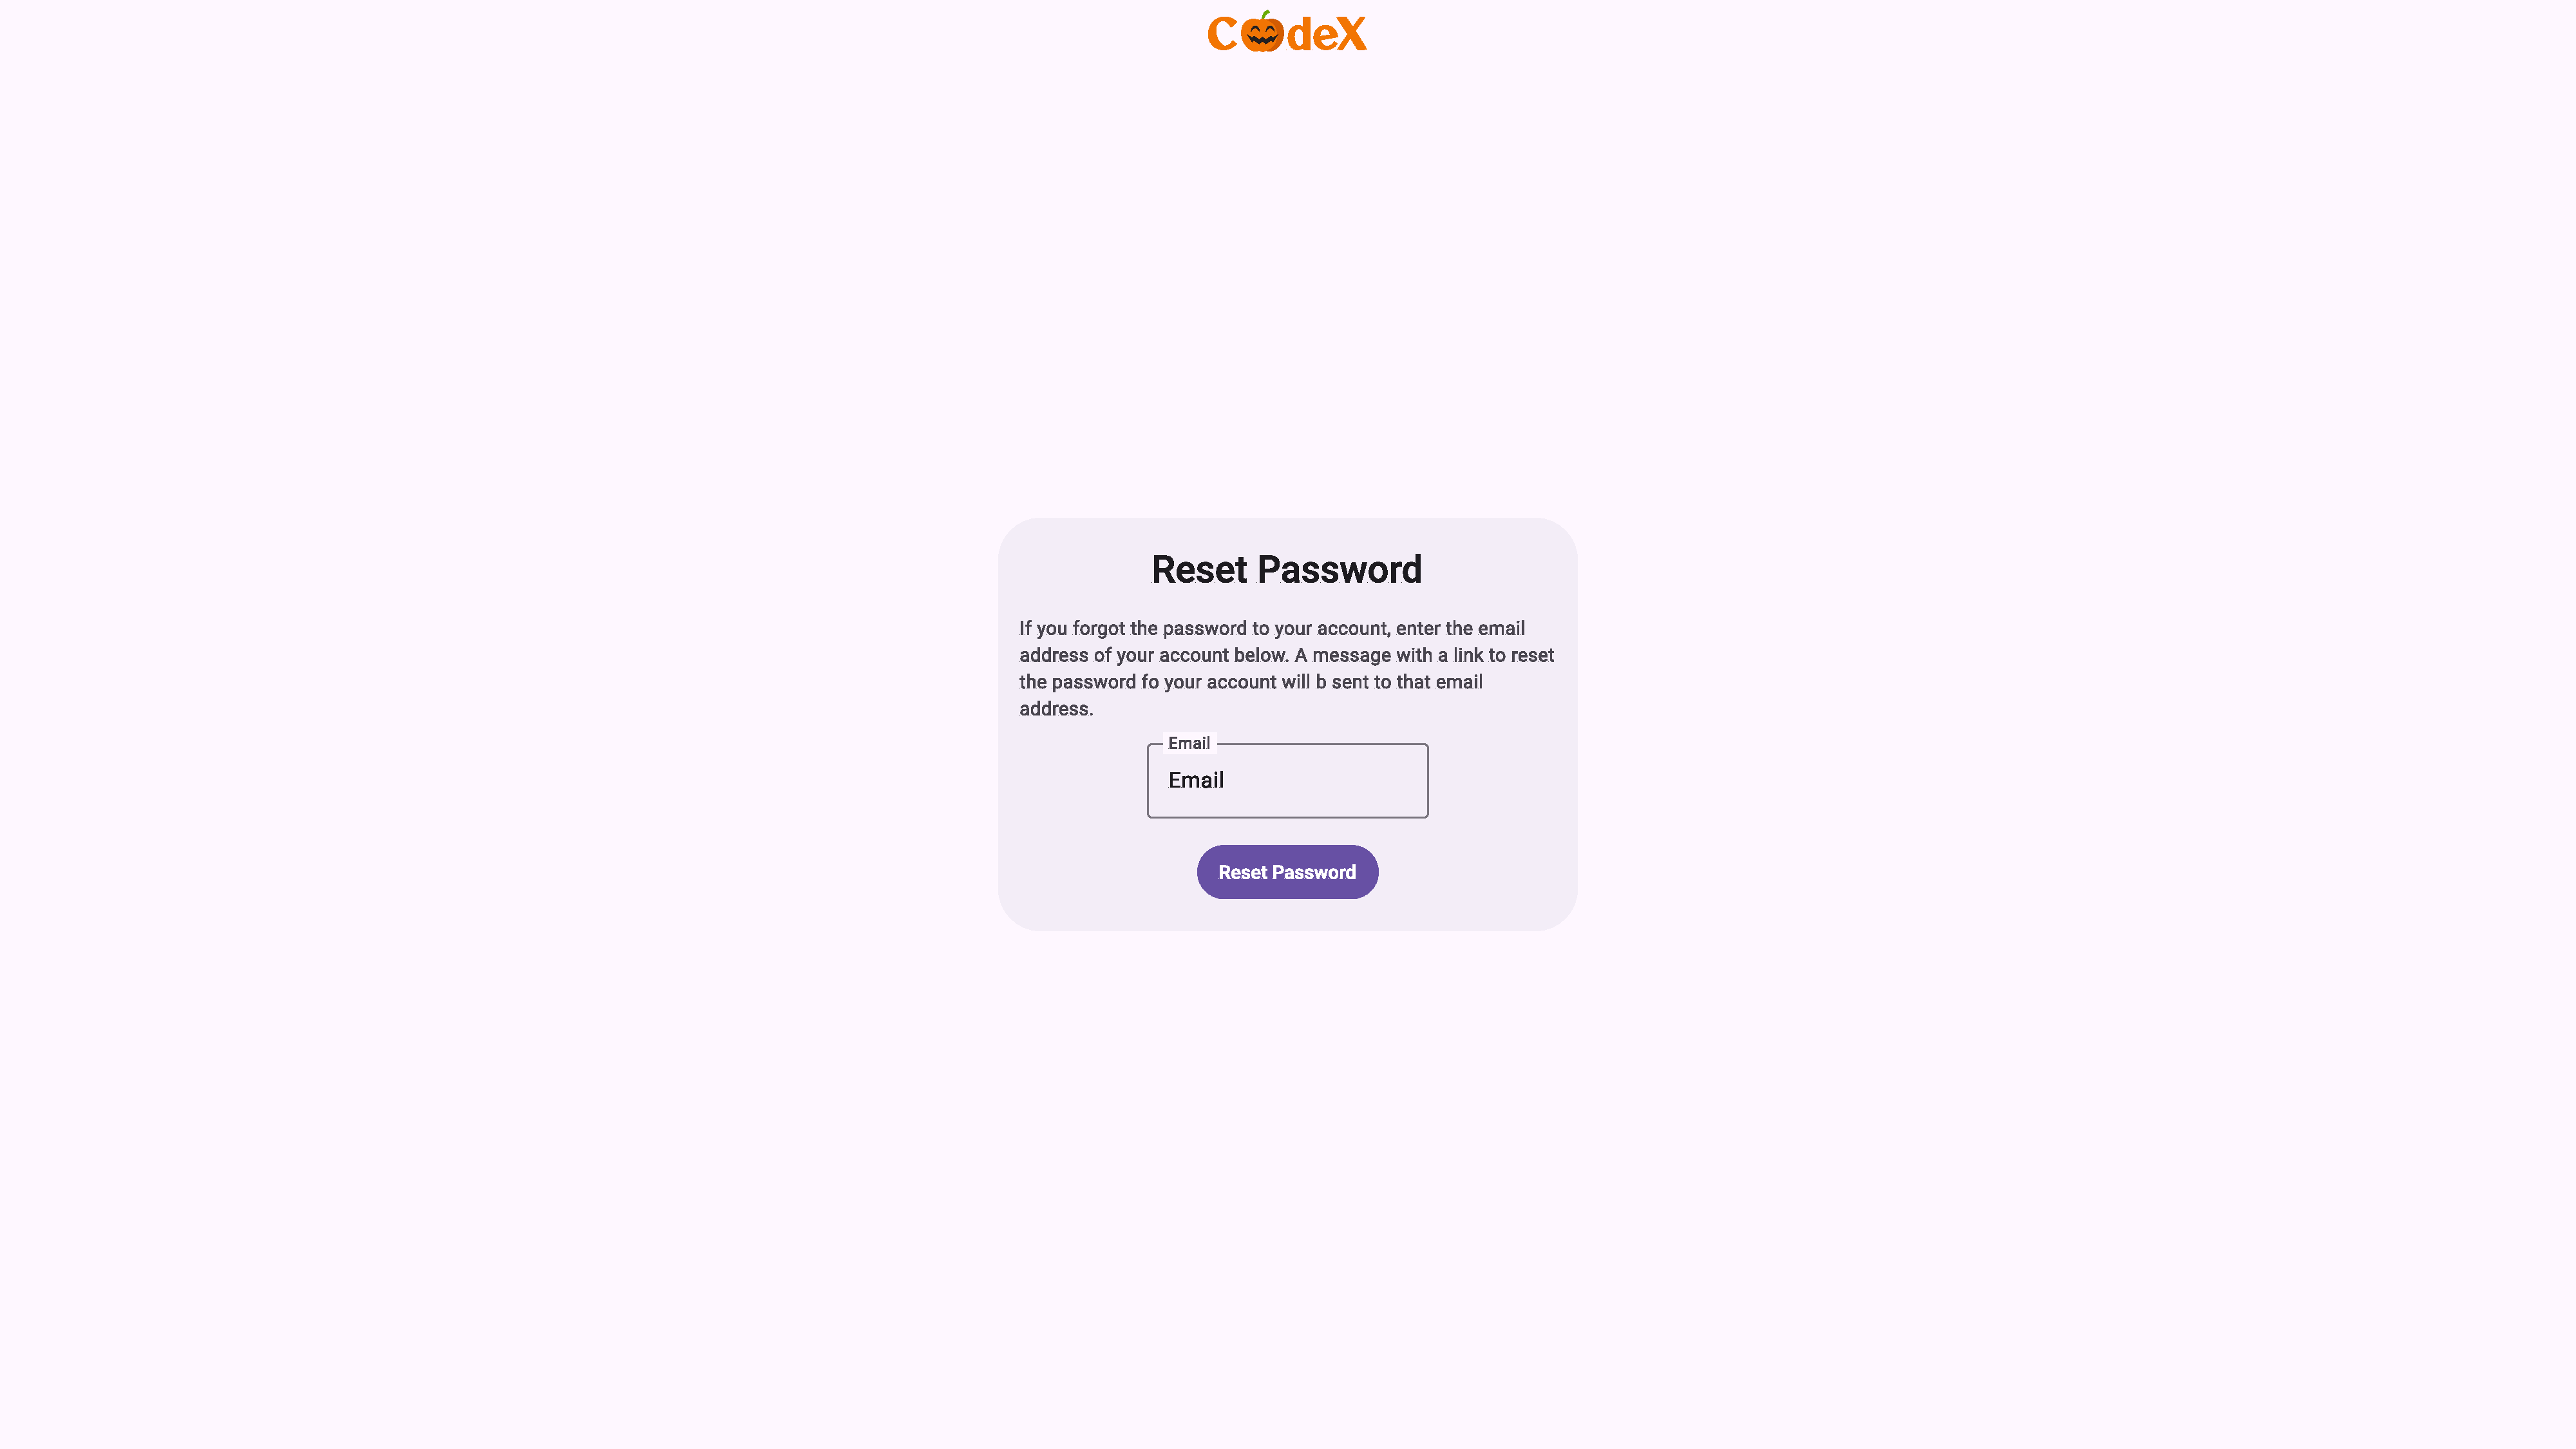
\includegraphics[width=\linewidth]{figures/ui/desktop/Request_Reset_Password_Screen initial}
    \caption{\hyperref[abr:GUI]{GUI}: Request password screen before requesting}
    \label{fig:ui-d-request-reset-password-initial}
\end{figure}
\begin{figure}
    \centering
    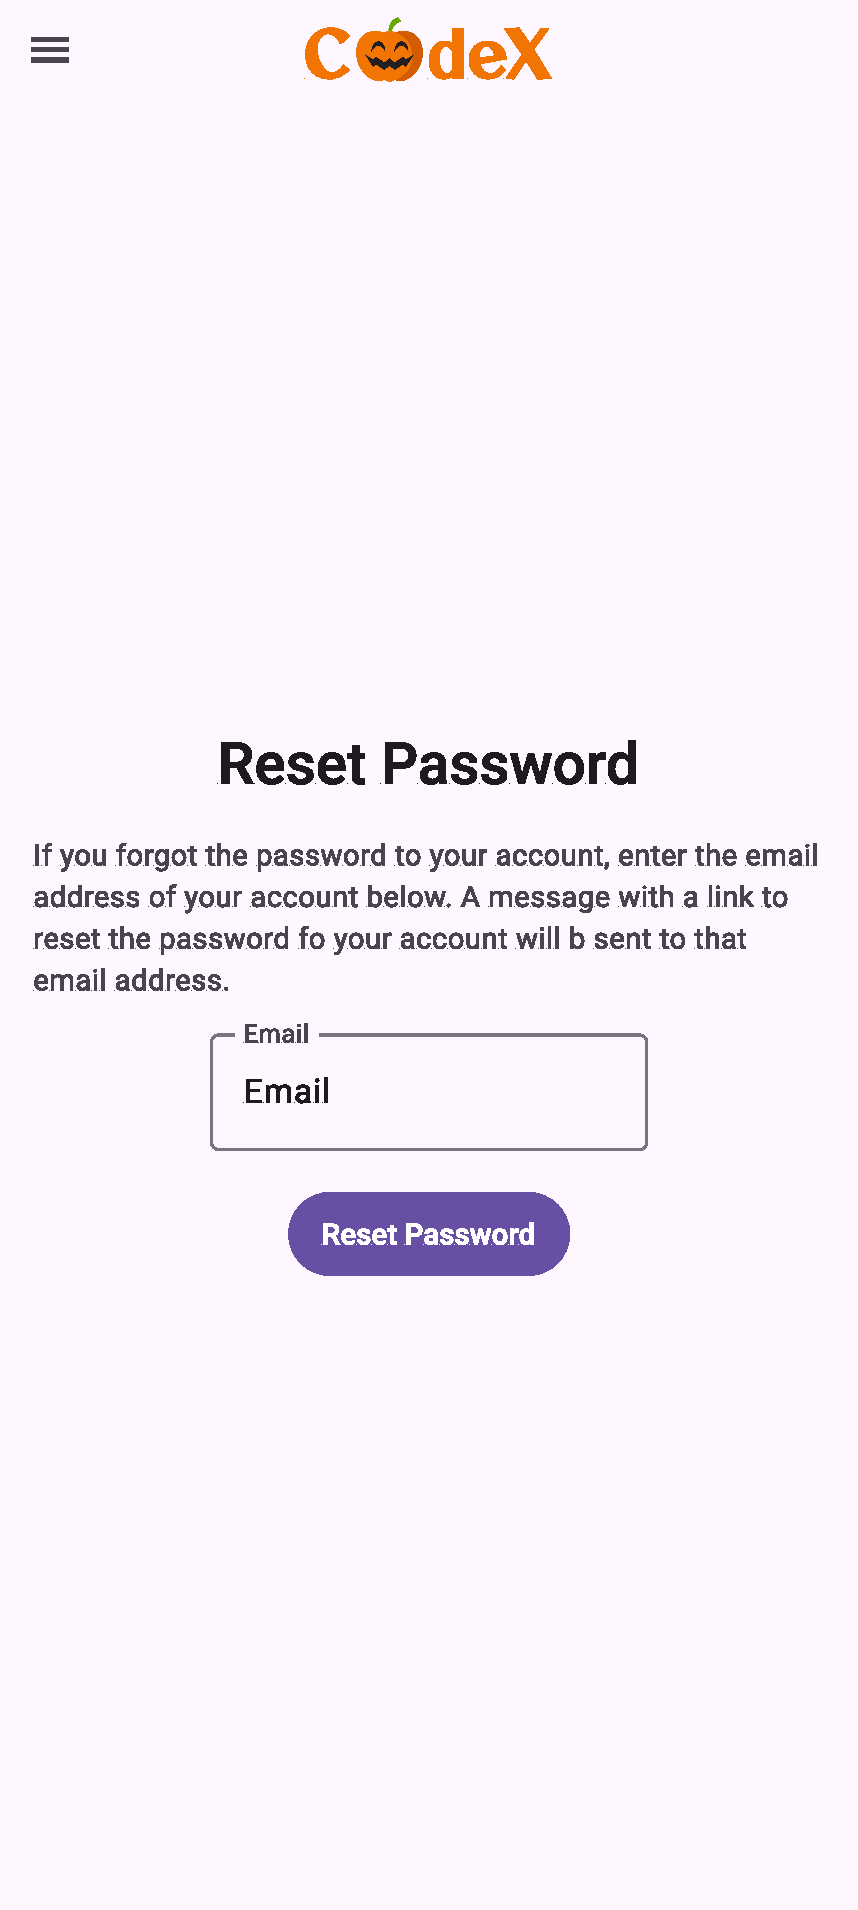
\includegraphics[width=5cm]{figures/ui/mobile/Request_Reset_Password_Screen initial}
    \caption{\hyperref[abr:GUI]{GUI}: Request password screen before requesting (mobile)}
    \label{fig:ui-m-request-reset-password-initial}
\end{figure}

\begin{figure}
    \centering
    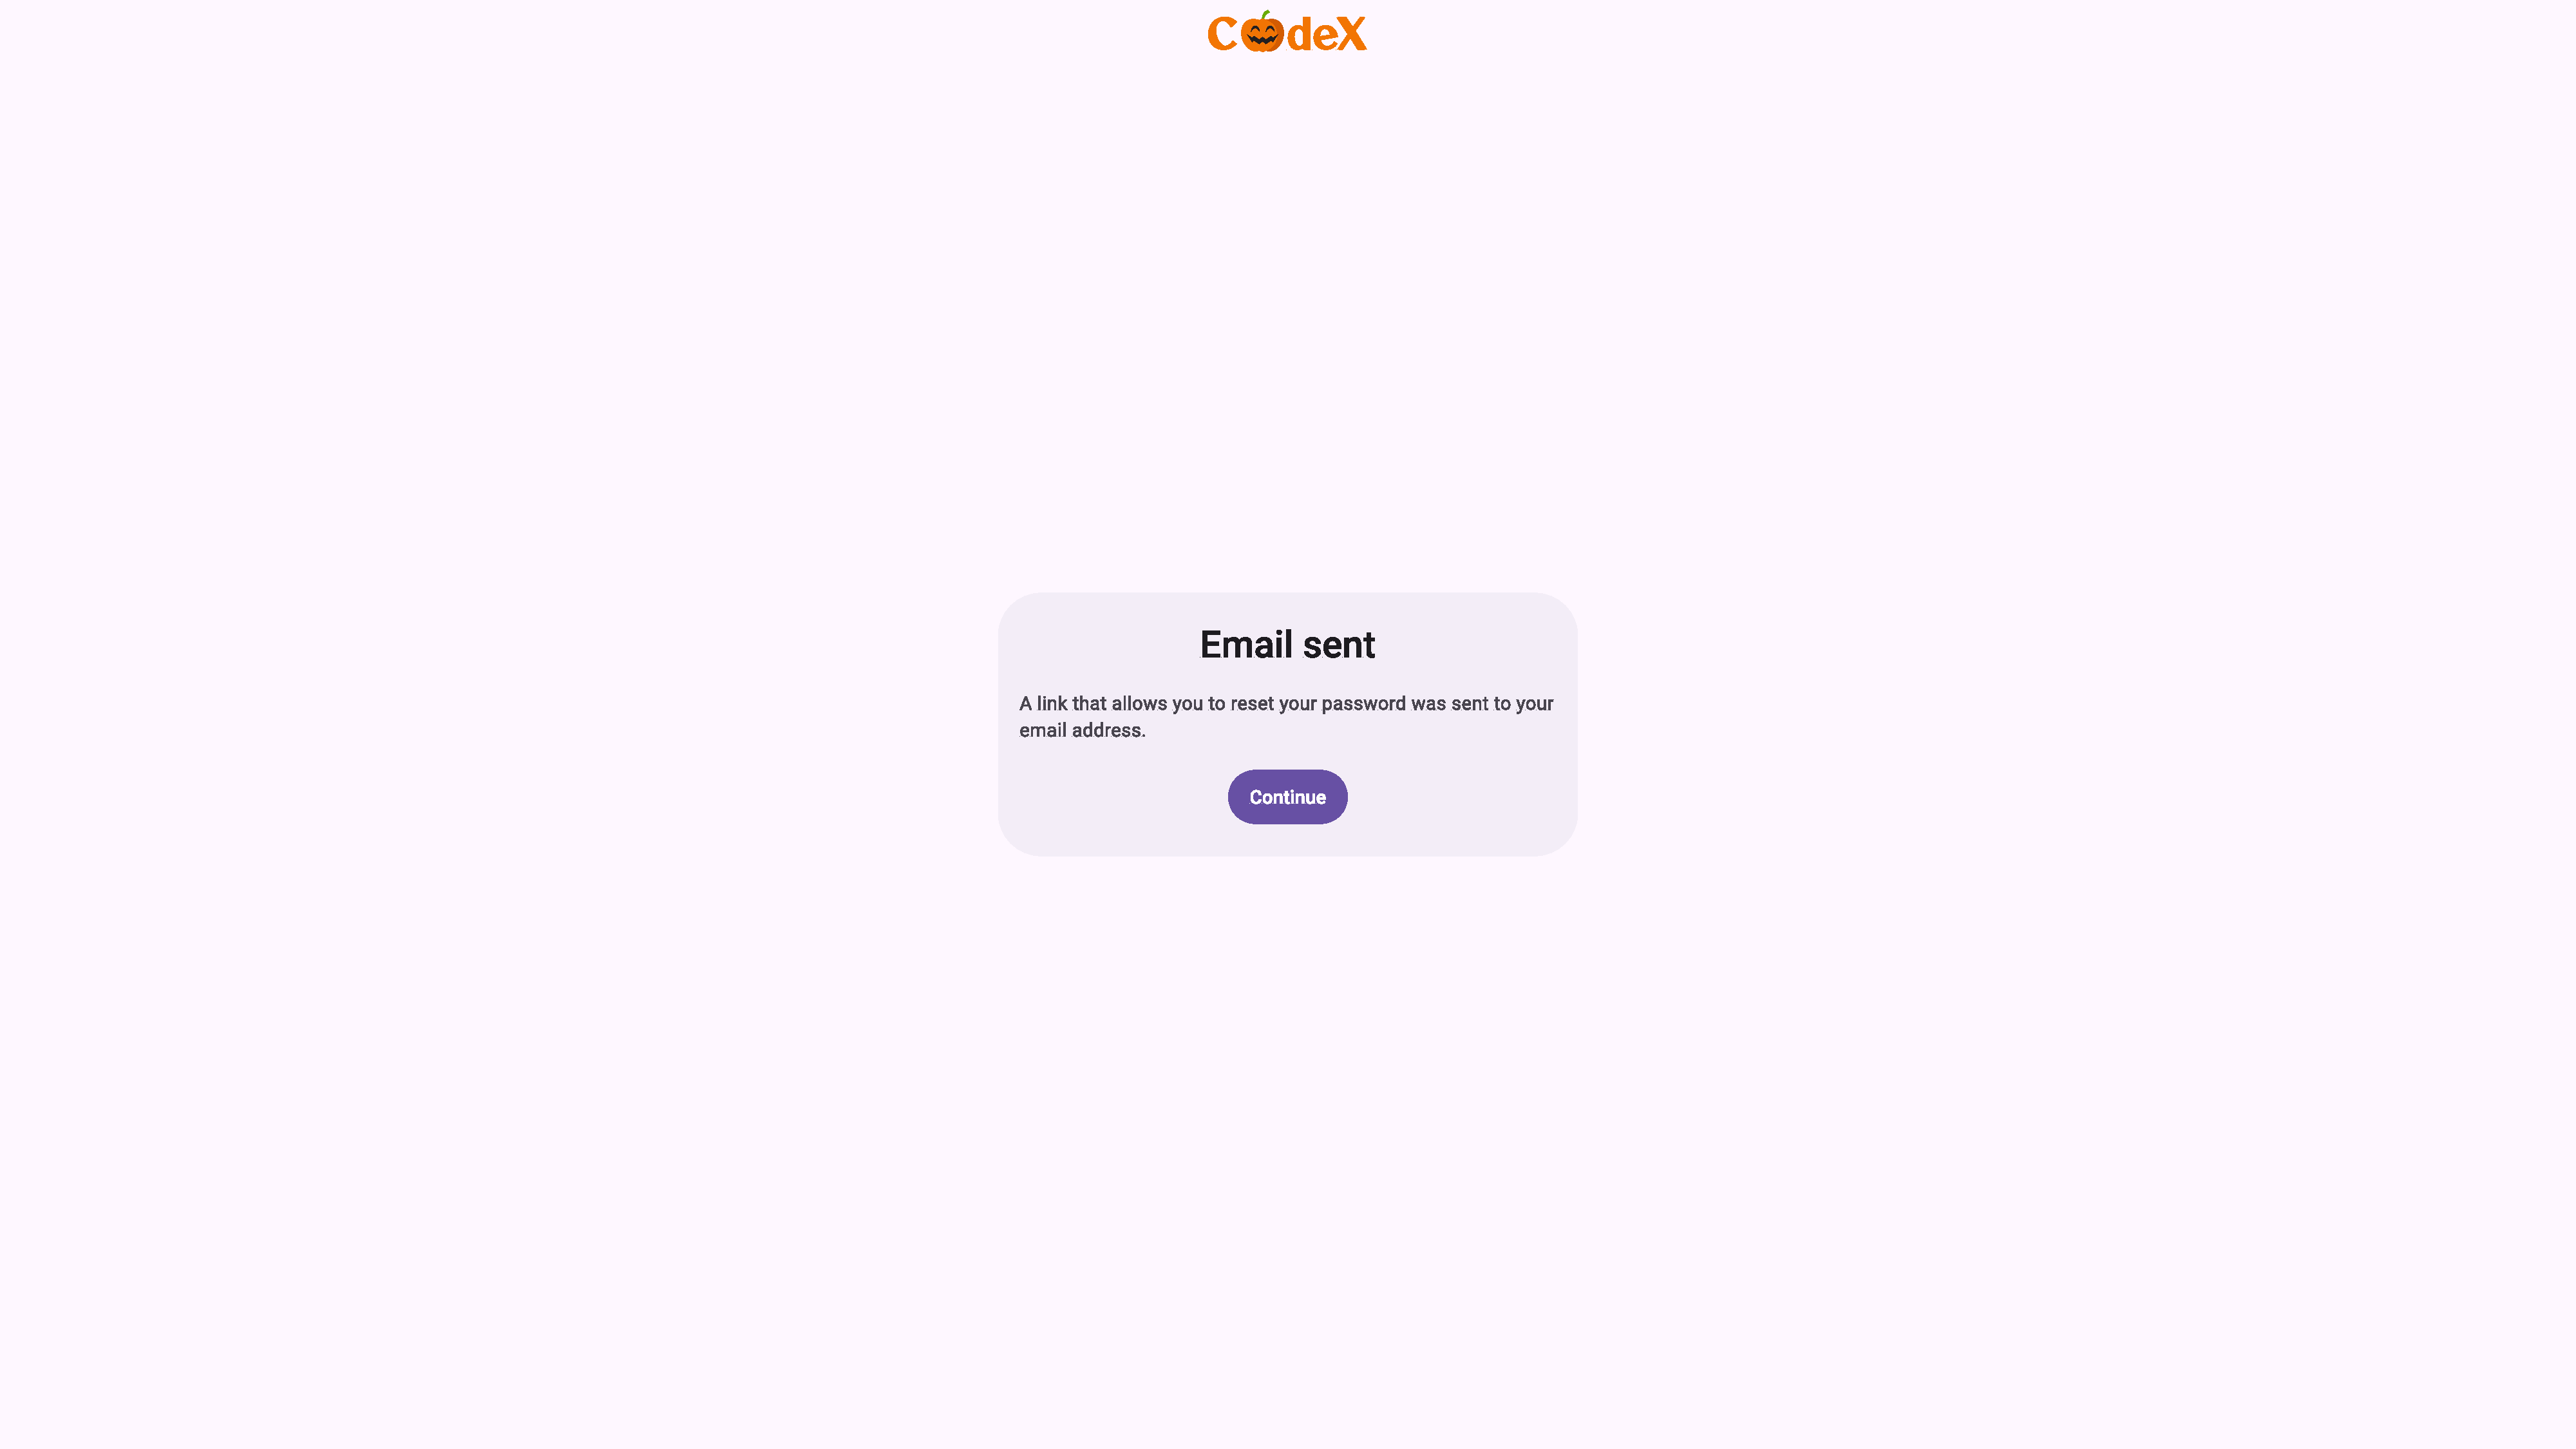
\includegraphics[width=\linewidth]{figures/ui/desktop/Request_Reset_Password_Screen requested}
    \caption{\hyperref[abr:GUI]{GUI}: Request password screen after requesting}
    \label{fig:ui-d-request-reset-password-requested}
\end{figure}
\begin{figure}
    \centering
    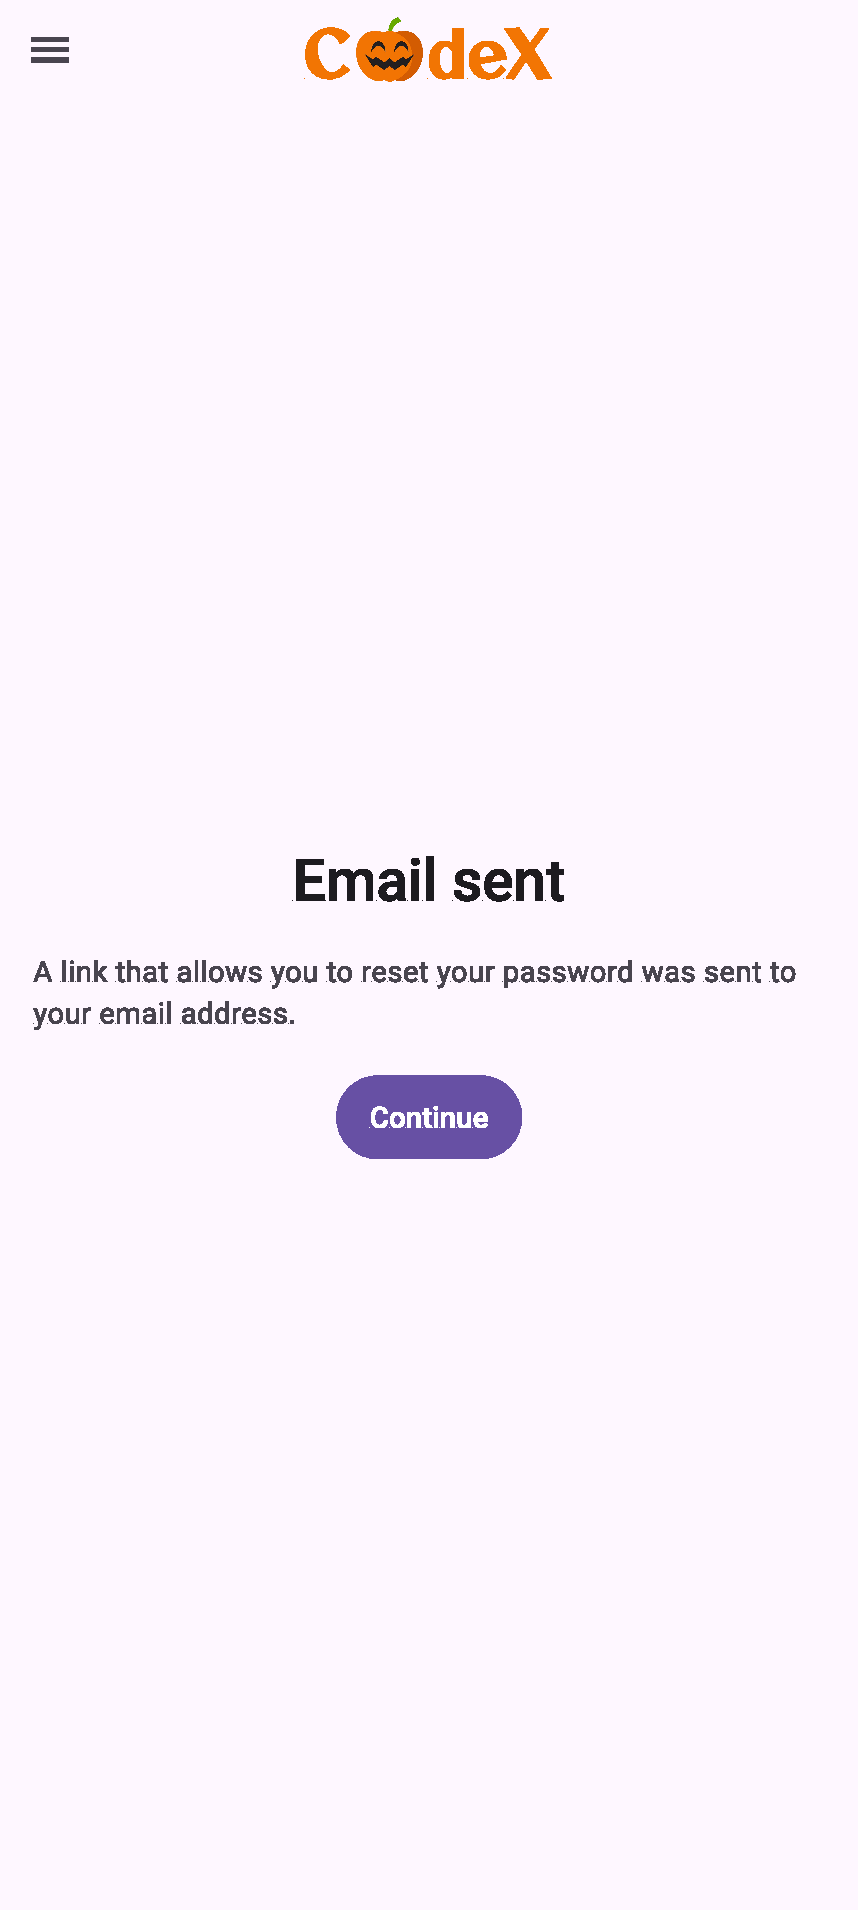
\includegraphics[width=5cm]{figures/ui/mobile/Request_Reset_Password_Screen requested}
    \caption{\hyperref[abr:GUI]{GUI}: Request password screen after requesting (mobile)}
    \label{fig:ui-m-request-reset-password-requested}
\end{figure}

\subsection{Password reset}
The password reset screen allows users to set a new password for their account.
This screen is reached by clicking the link that the user received via mail. \newline
Users can enter a new password (\ref{fig:ui-d-reset-password-initial}/\ref{fig:ui-m-reset-password-initial}), after which an informative message is shown (\ref{fig:ui-d-reset-password-reset}/\ref{fig:ui-m-reset-password-reset}).
\begin{figure}
    \centering
    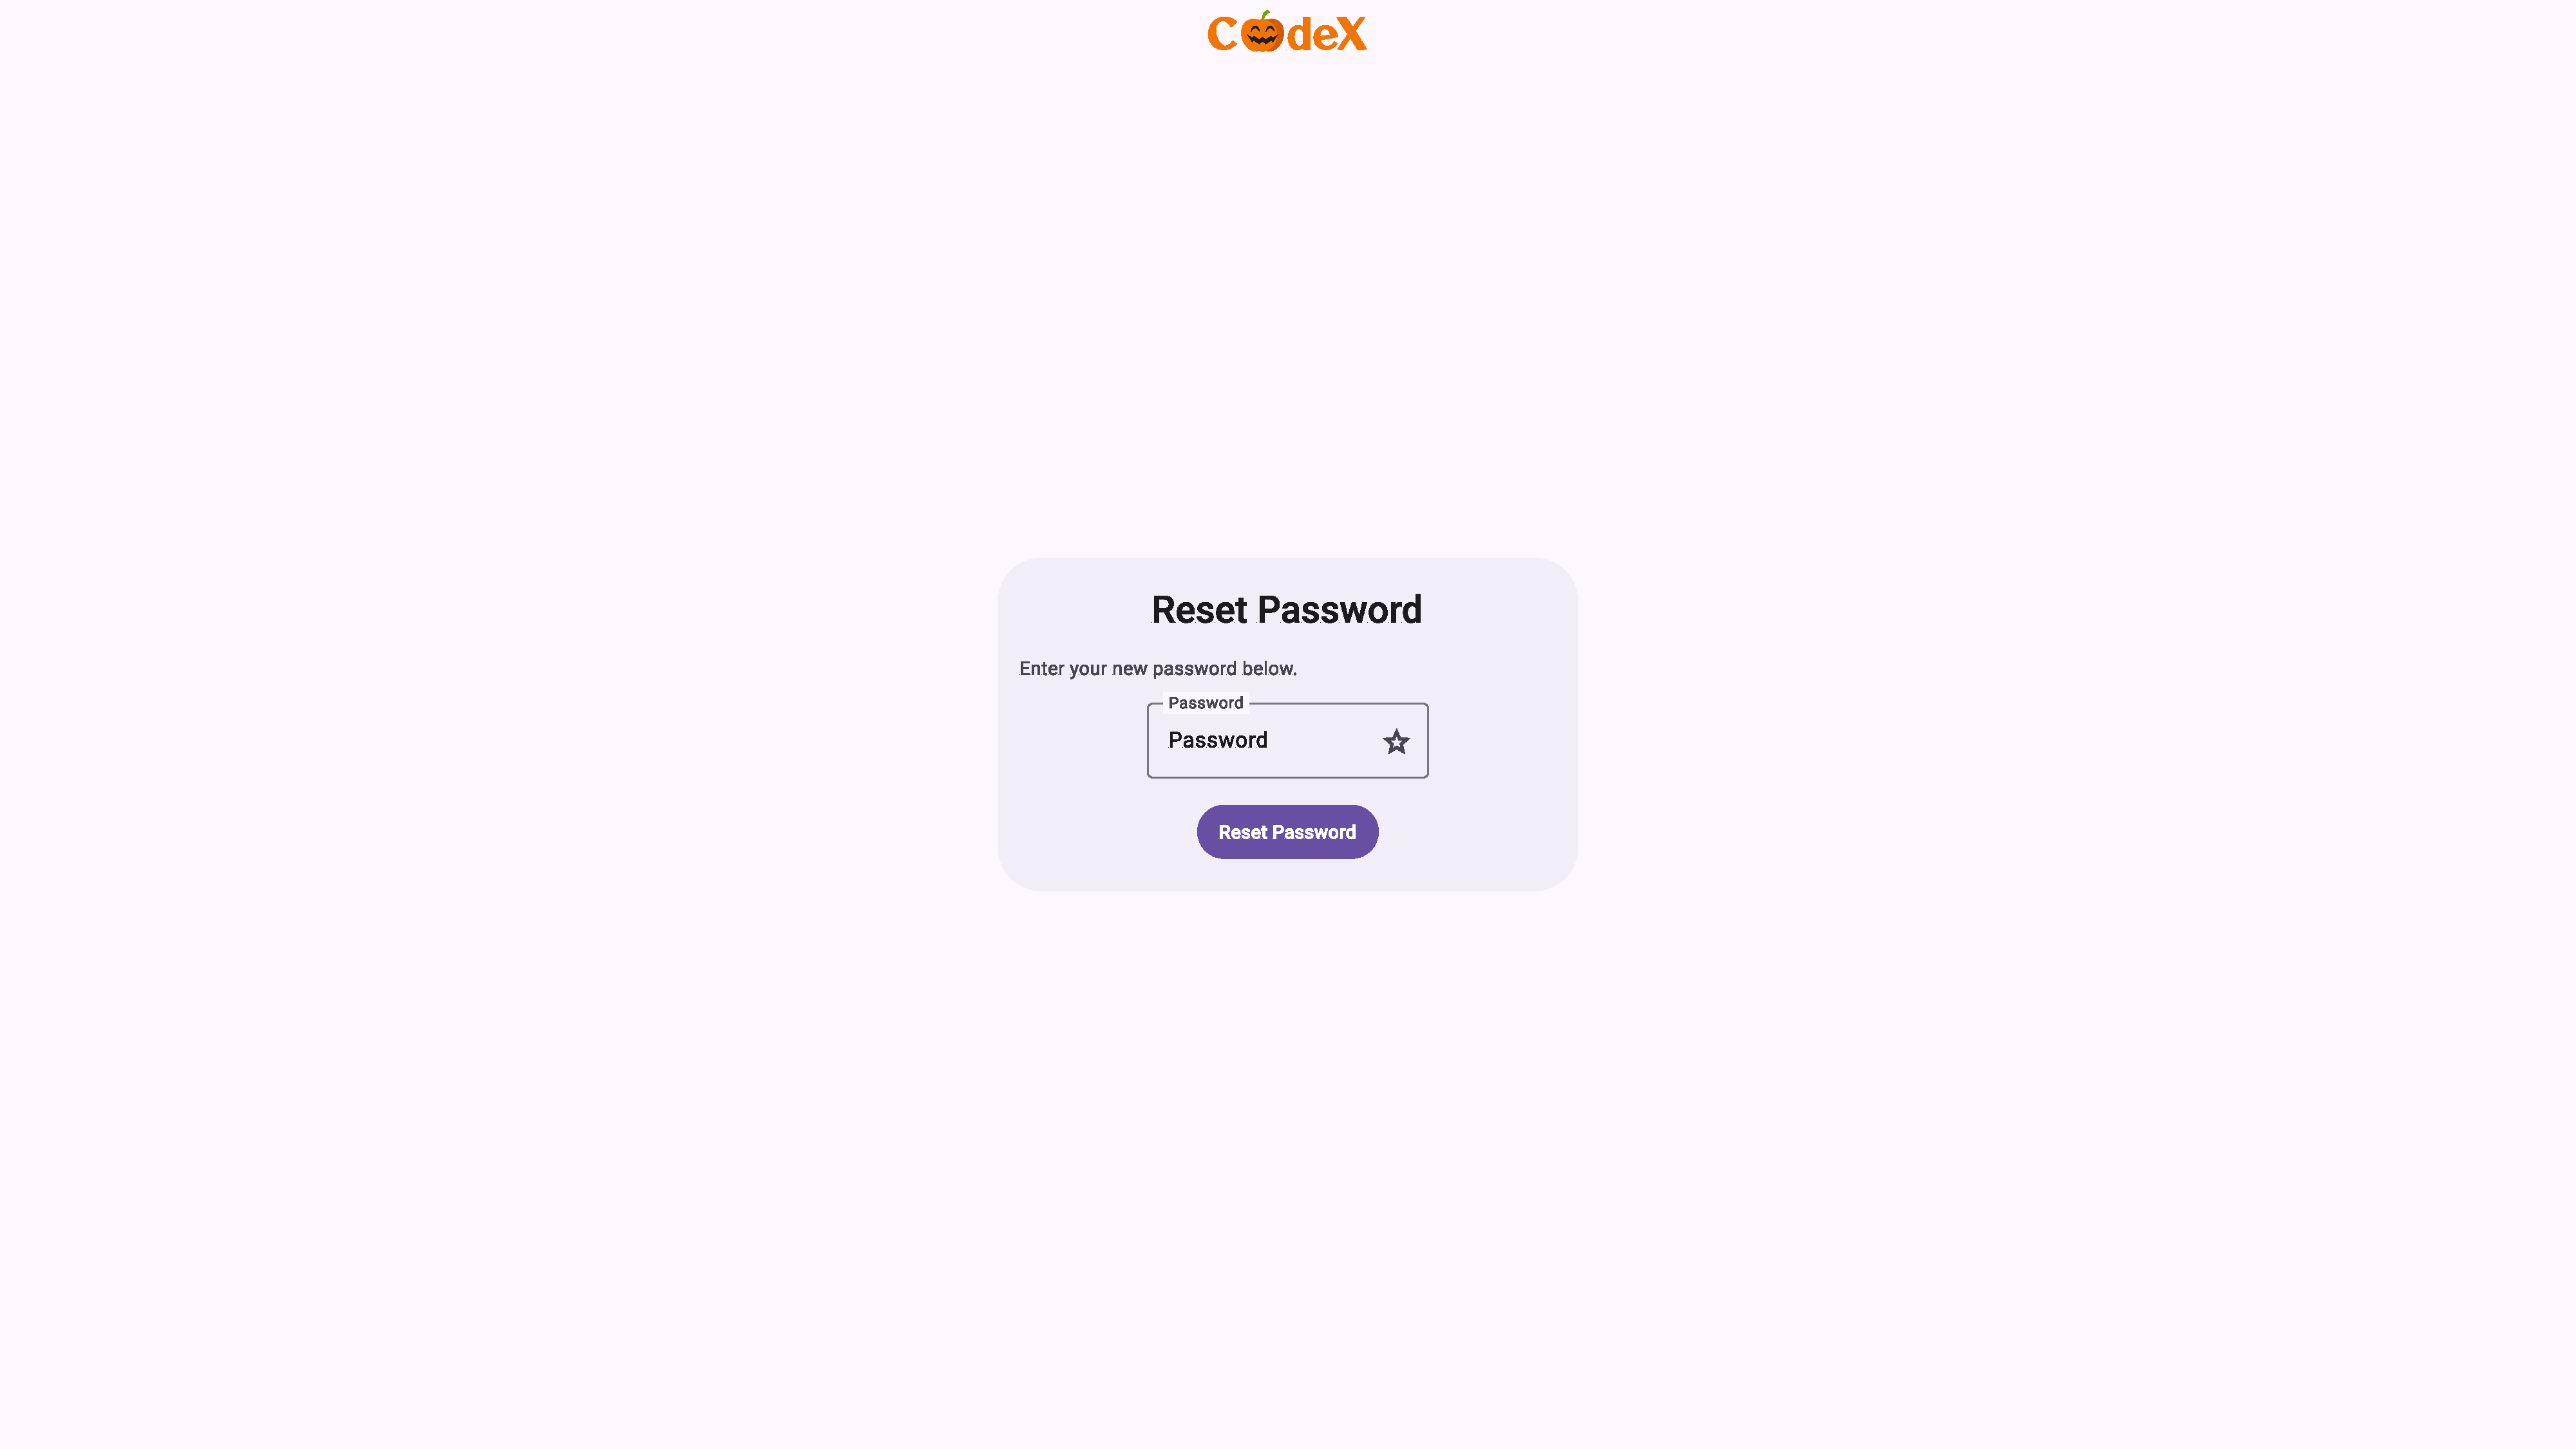
\includegraphics[width=\linewidth]{figures/ui/desktop/Reset_Password_Screen initial}
    \caption{\hyperref[abr:GUI]{GUI}: Reset password screen}
    \label{fig:ui-d-reset-password-initial}
\end{figure}
\begin{figure}
    \centering
    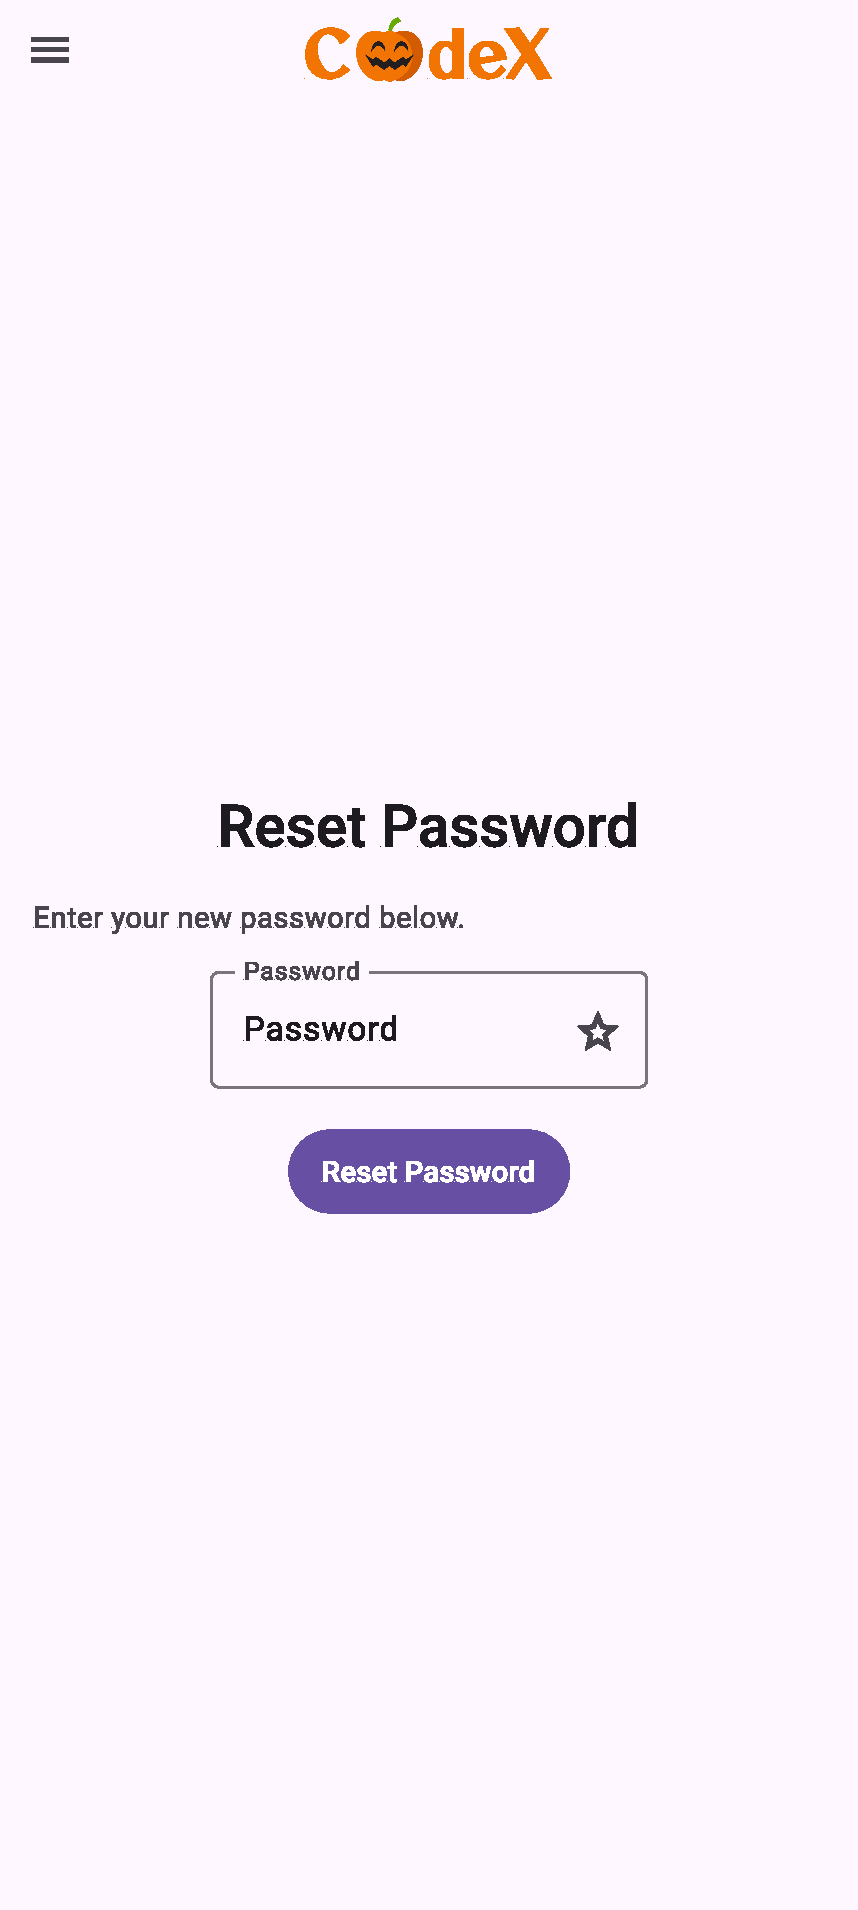
\includegraphics[width=5cm]{figures/ui/mobile/Reset_Password_Screen initial}
    \caption{\hyperref[abr:GUI]{GUI}: Reset password screen (mobile)}
    \label{fig:ui-m-reset-password-initial}
\end{figure}

\begin{figure}
    \centering
    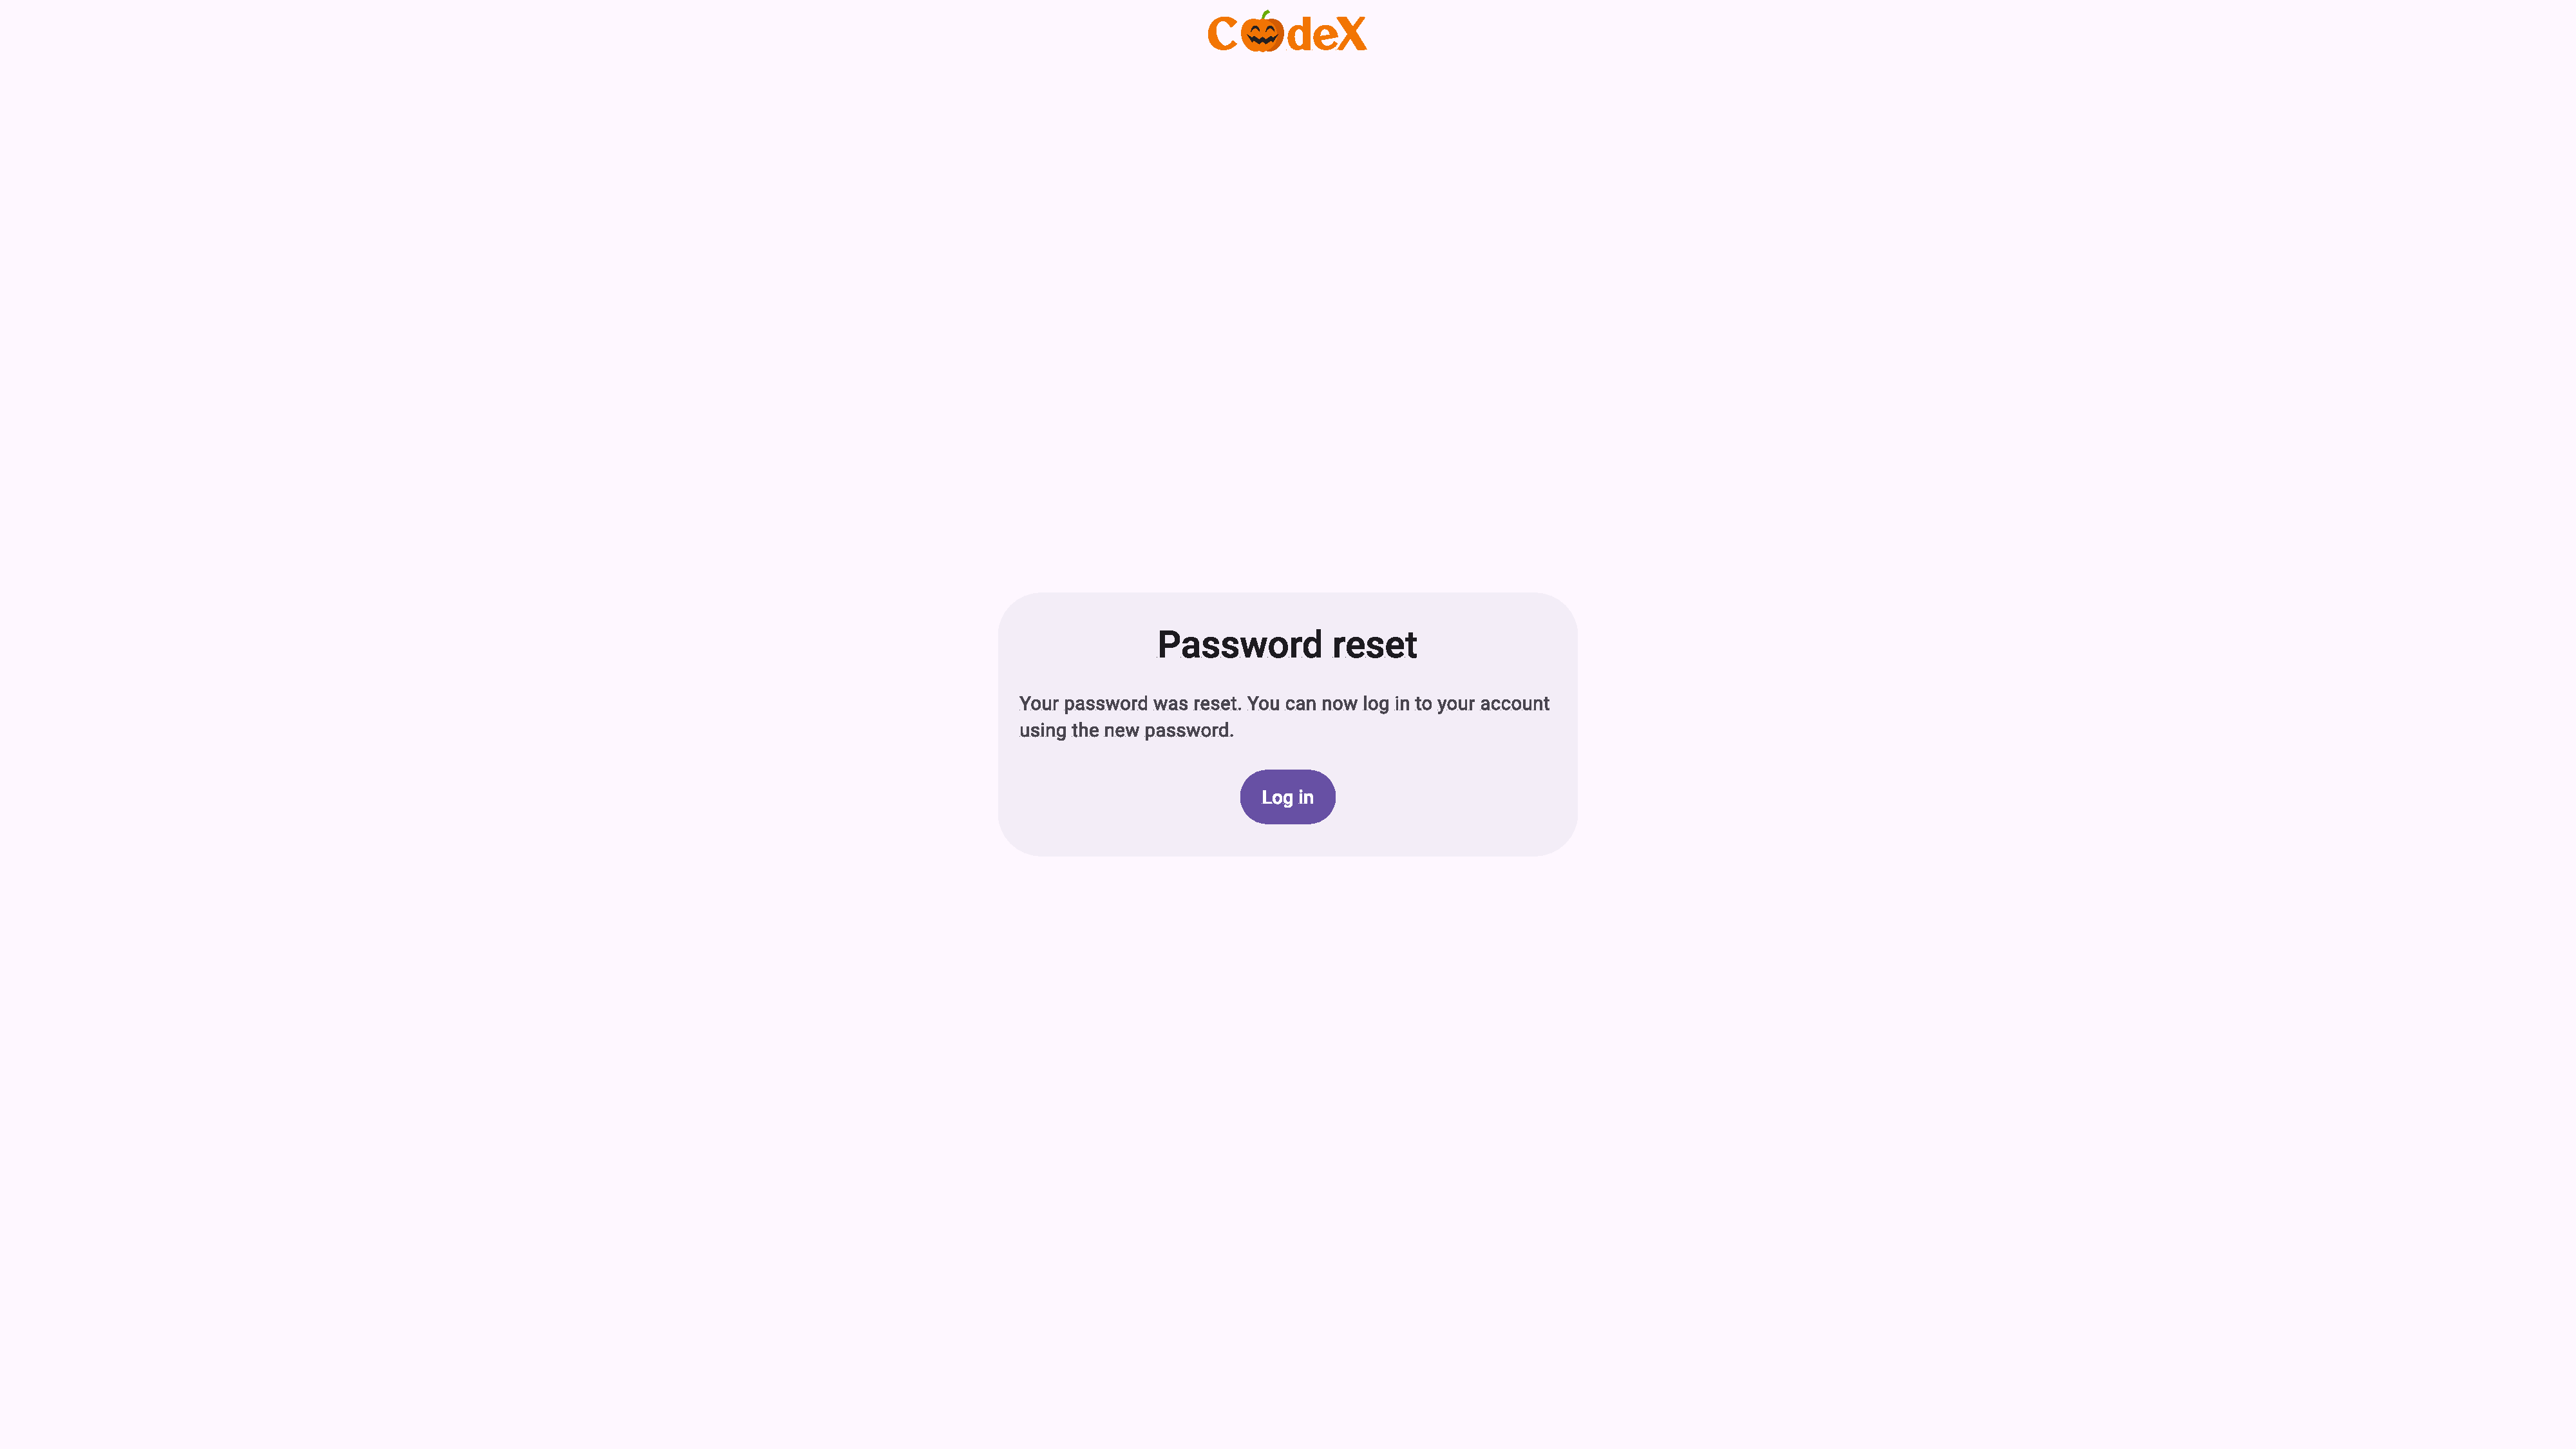
\includegraphics[width=\linewidth]{figures/ui/desktop/Reset_Password_Screen resetted}
    \caption{\hyperref[abr:GUI]{GUI}: Reset password screen after the password was set}
    \label{fig:ui-d-reset-password-reset}
\end{figure}
\begin{figure}
    \centering
    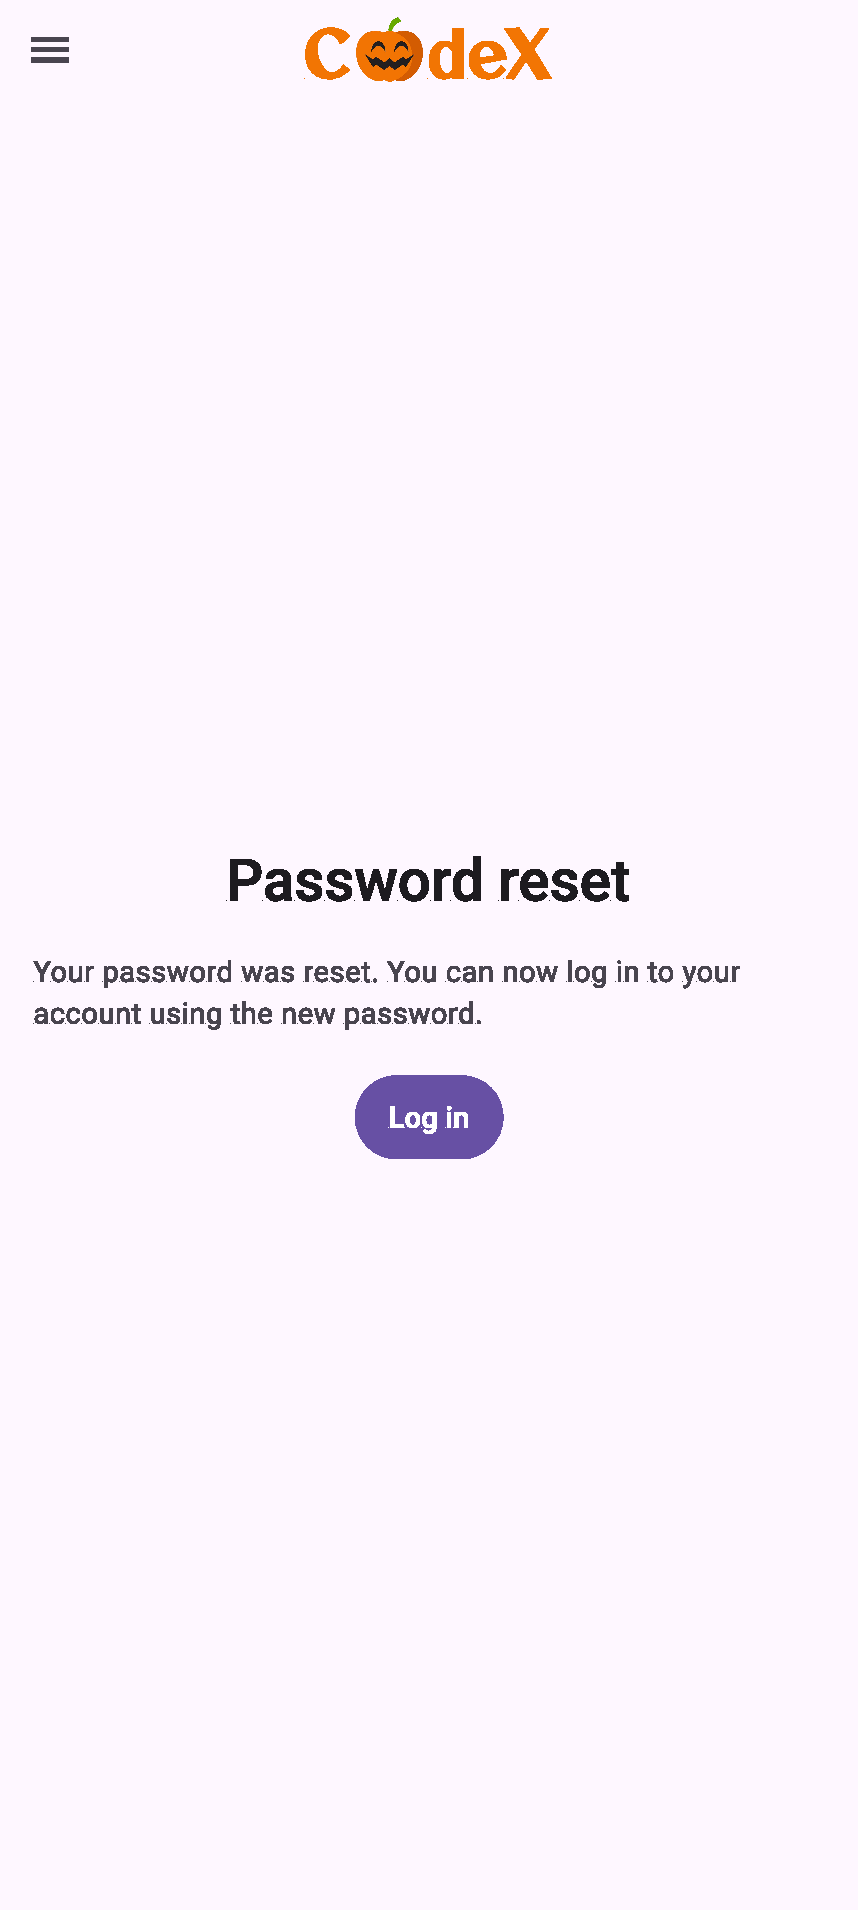
\includegraphics[width=5cm]{figures/ui/mobile/Reset_Password_Screen resetted}
    \caption{\hyperref[abr:GUI]{GUI}: Reset password screen after the password was set (mobile)}
    \label{fig:ui-m-reset-password-reset}
\end{figure}

\subsection{Signup}
The signup screen (\ref{fig:ui-d-signup}/\ref{fig:ui-m-signup}) allows a user to create a new account by entering email, username and a password. \newline
The screen also provides options to log in instead, or to use an \textit{\hyperref[def:oauth]{OAuth} provider}.
\begin{figure}
    \centering
    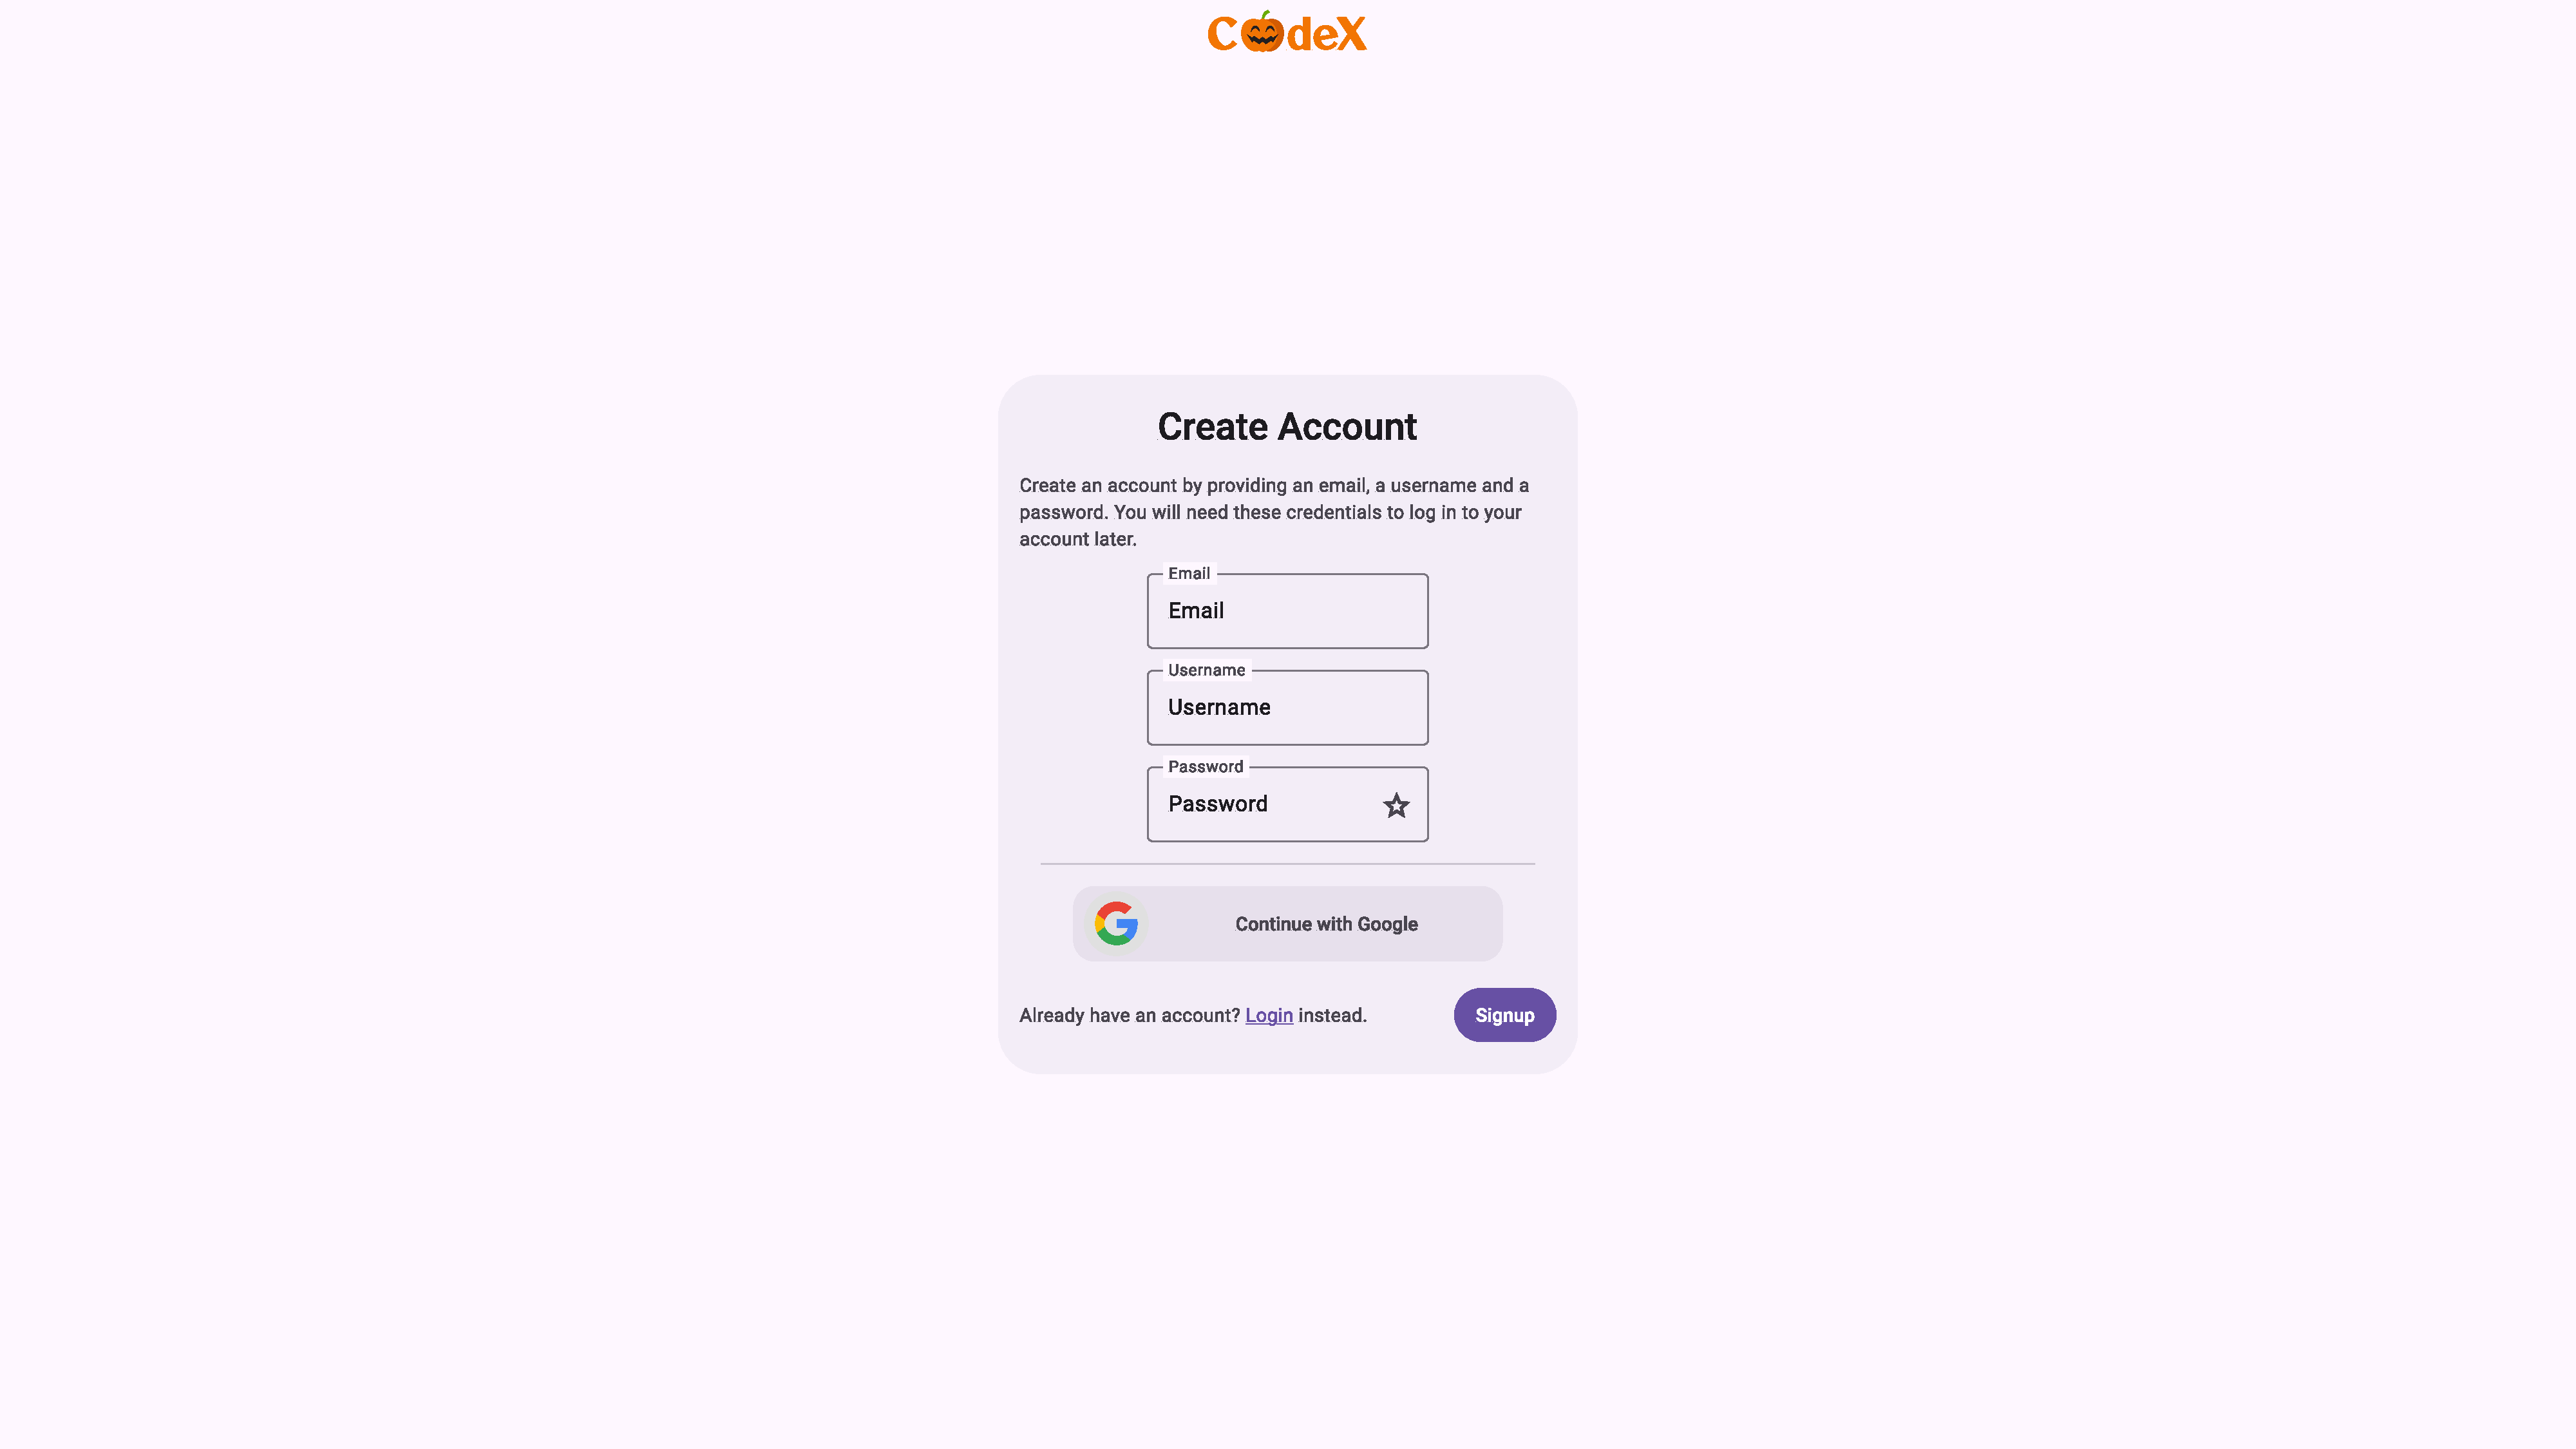
\includegraphics[width=\linewidth]{figures/ui/desktop/Signup_Screen}
    \caption{\hyperref[abr:GUI]{GUI}: Signup screen}
    \label{fig:ui-d-signup}
\end{figure}
\begin{figure}
    \centering
    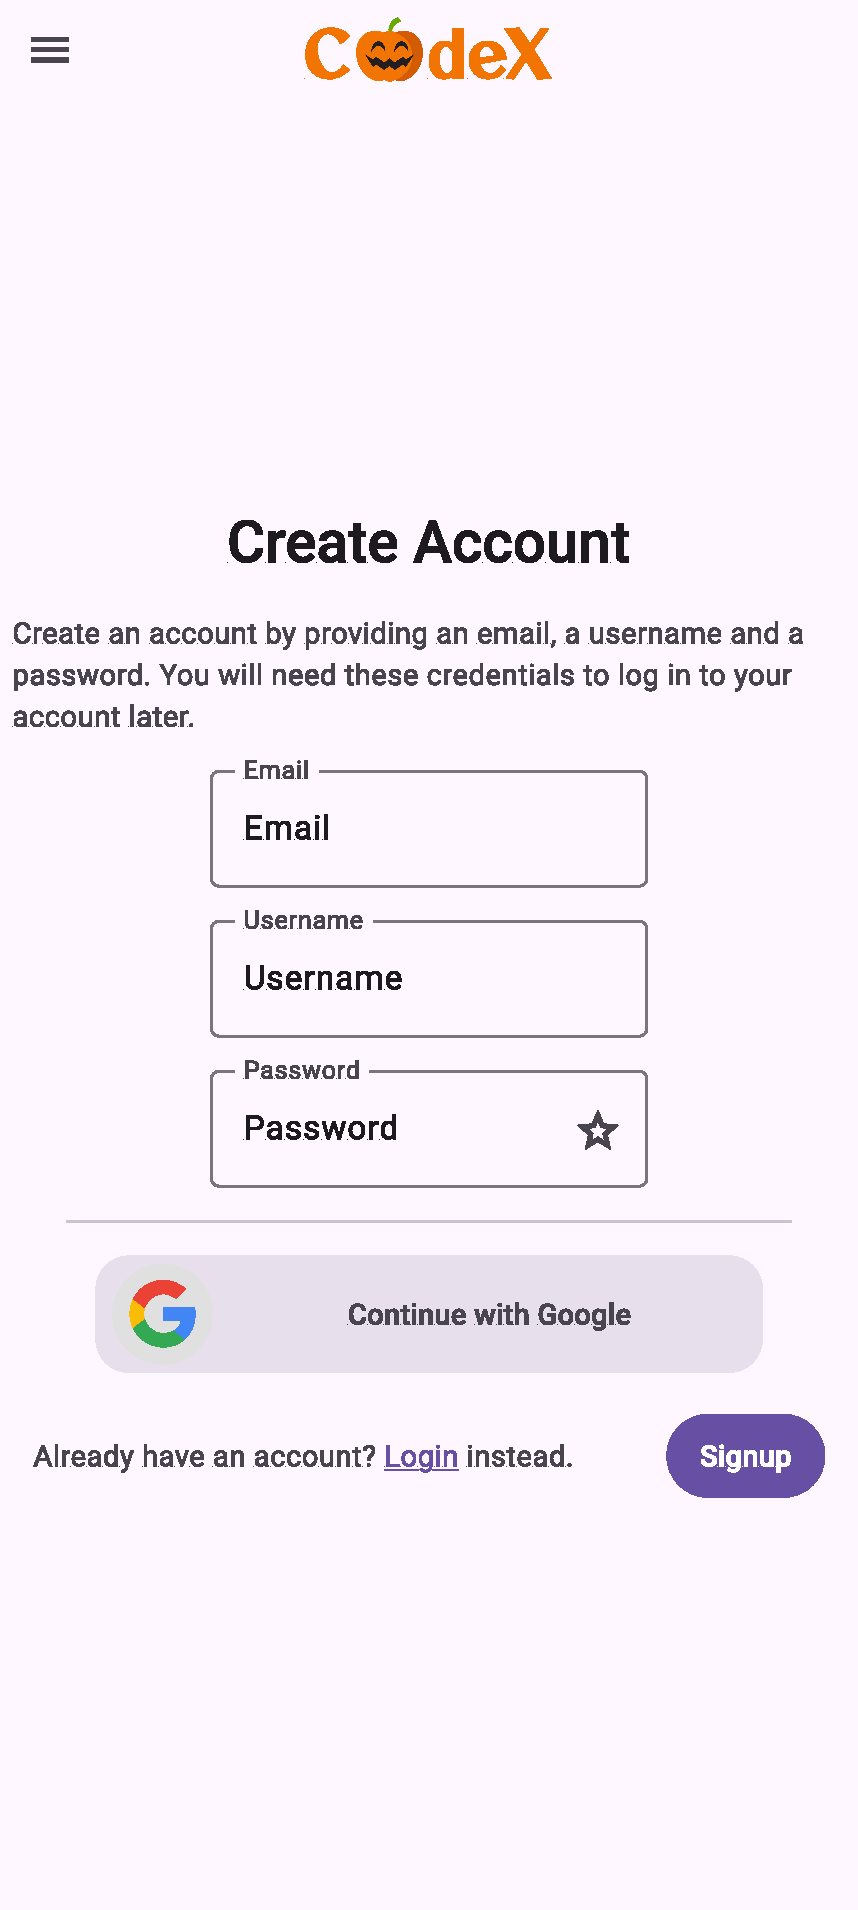
\includegraphics[width=5cm]{figures/ui/mobile/Signup_Screen}
    \caption{\hyperref[abr:GUI]{GUI}: Signup screen (mobile)}
    \label{fig:ui-m-signup}
\end{figure}

\subsection{Not verified screen}
The not verified screen is shown to authenticated users that try to perform an action that requires their email to be verified. \newline
Users have the option to request a verification message (\ref{fig:ui-d-not-verified-initial}/\ref{fig:ui-m-not-verified-initial}), after which an informative message is shown (\ref{fig:ui-d-not-verified-requested}/\ref{fig:ui-m-not-verified-requested}).
\begin{figure}
    \centering
    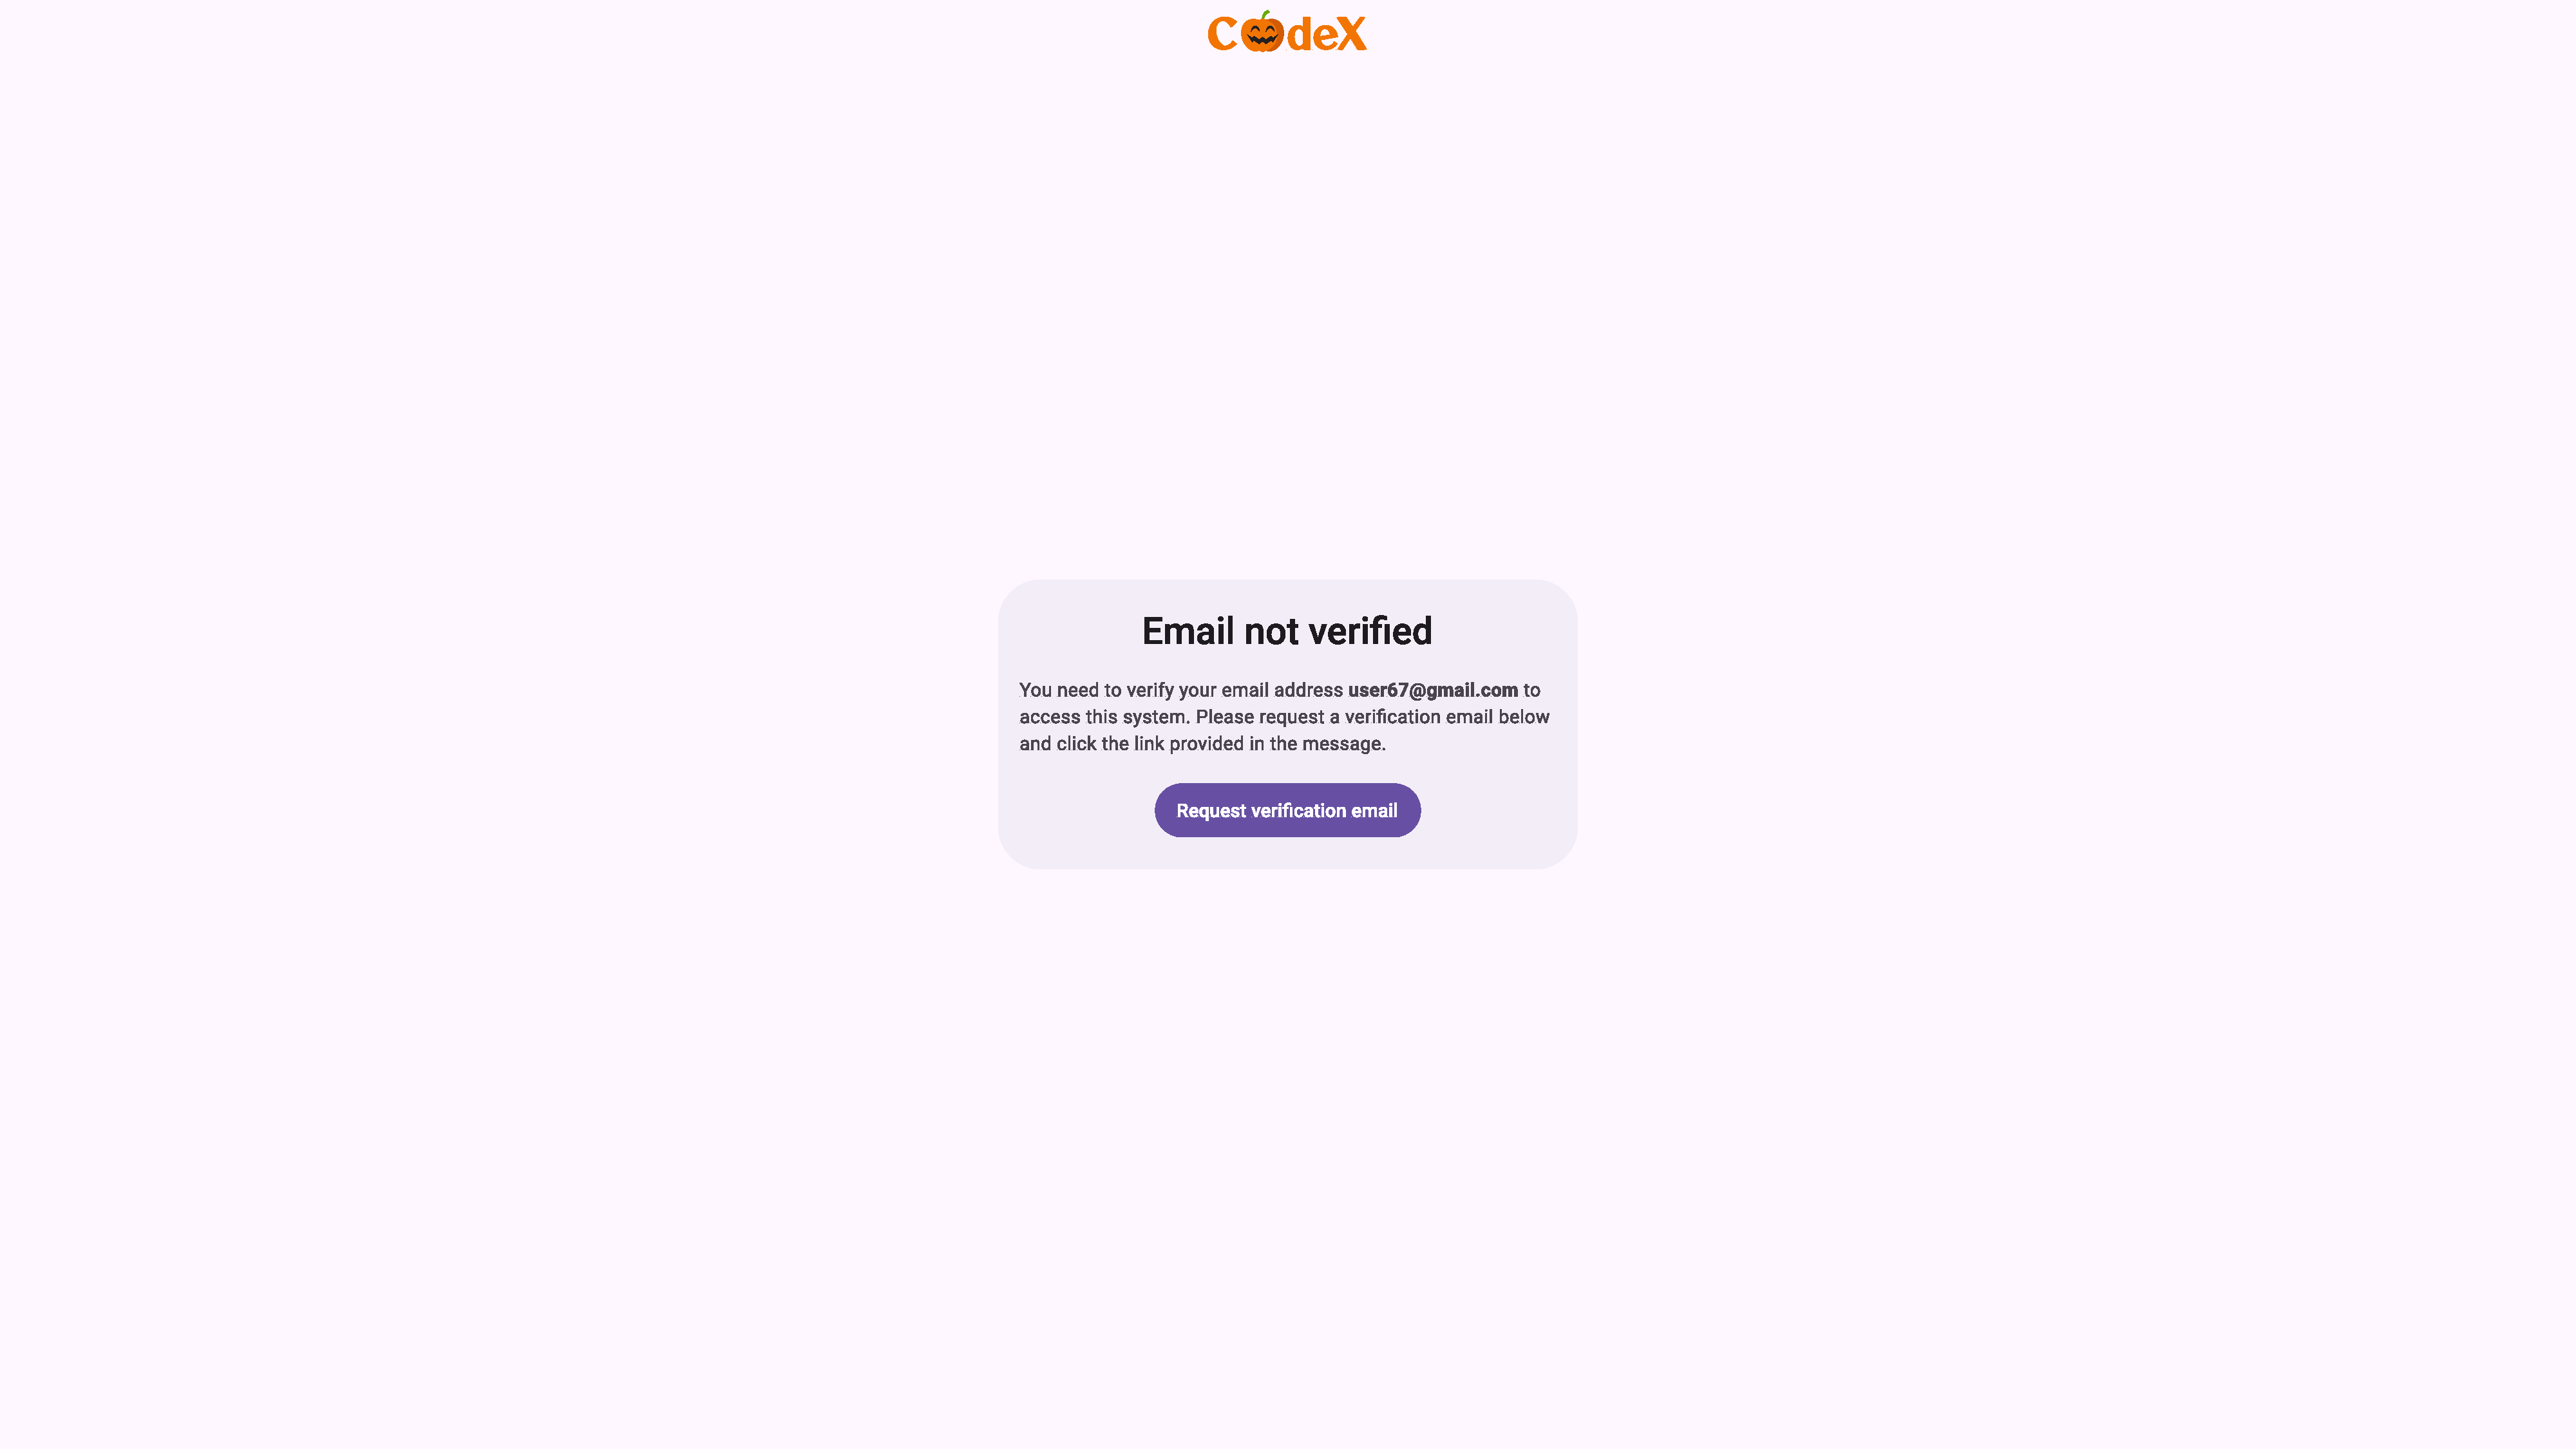
\includegraphics[width=\linewidth]{figures/ui/desktop/Not_Verified_Screen initial}
    \caption{\hyperref[abr:GUI]{GUI}: Not verified screen}
    \label{fig:ui-d-not-verified-initial}
\end{figure}
\begin{figure}
    \centering
    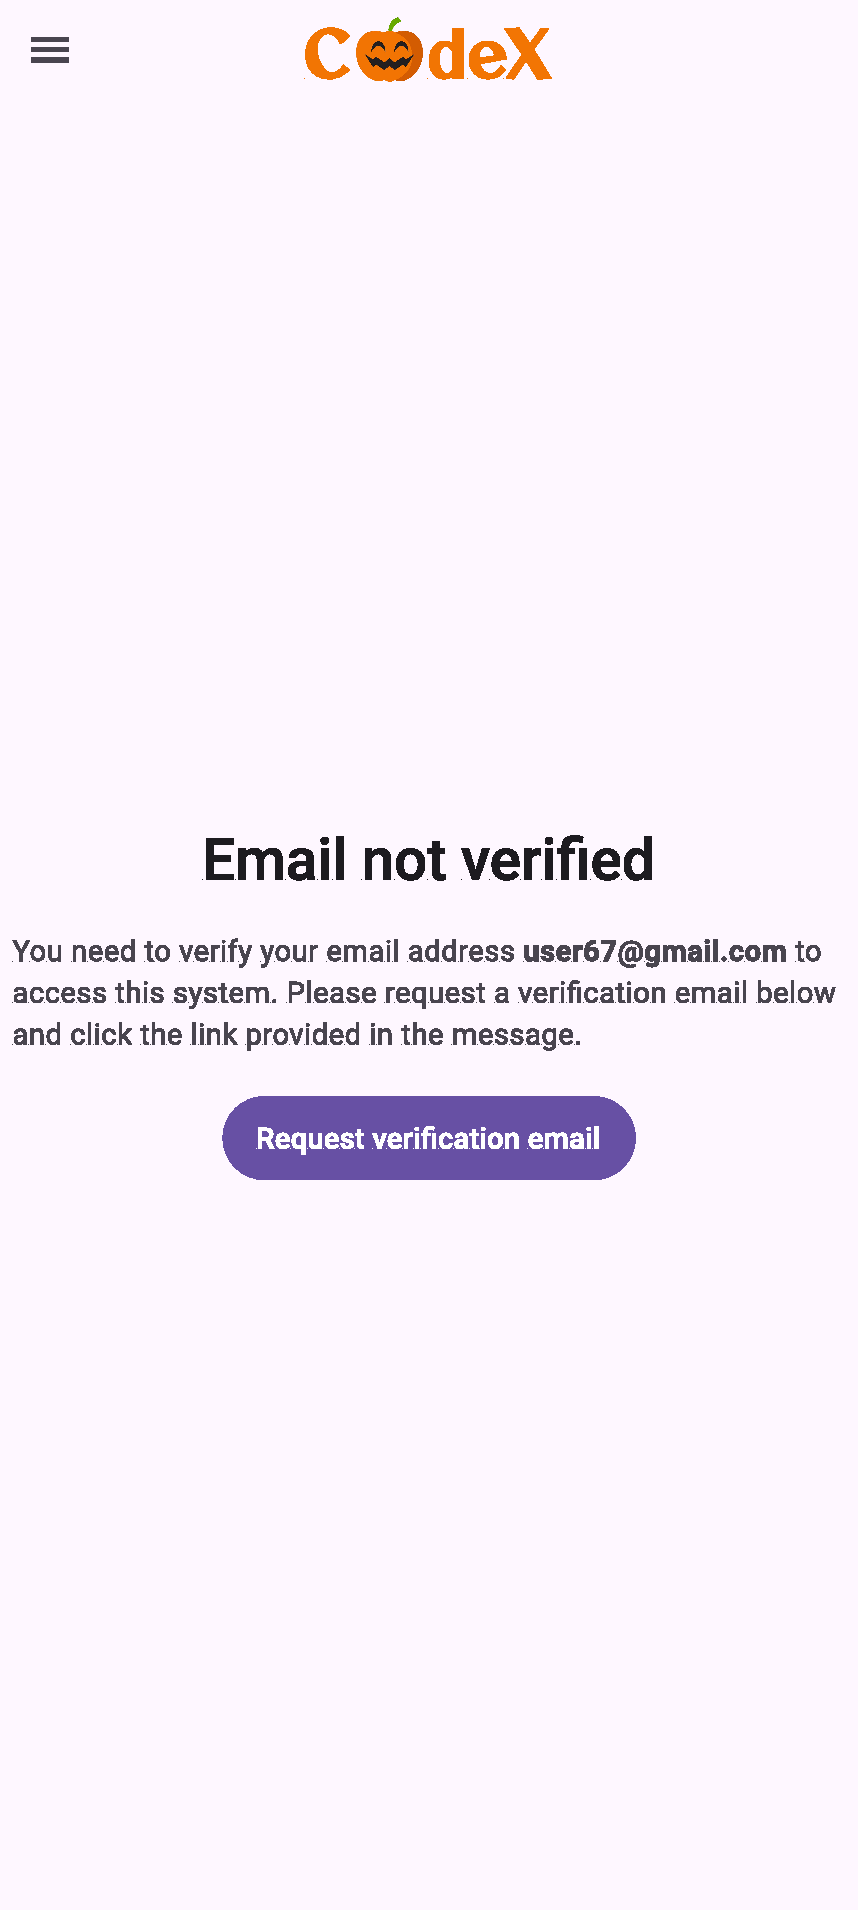
\includegraphics[width=5cm]{figures/ui/mobile/Not_Verified_Screen initial}
    \caption{\hyperref[abr:GUI]{GUI}: Not verified screen (mobile)}
    \label{fig:ui-m-not-verified-initial}
\end{figure}

\begin{figure}
    \centering
    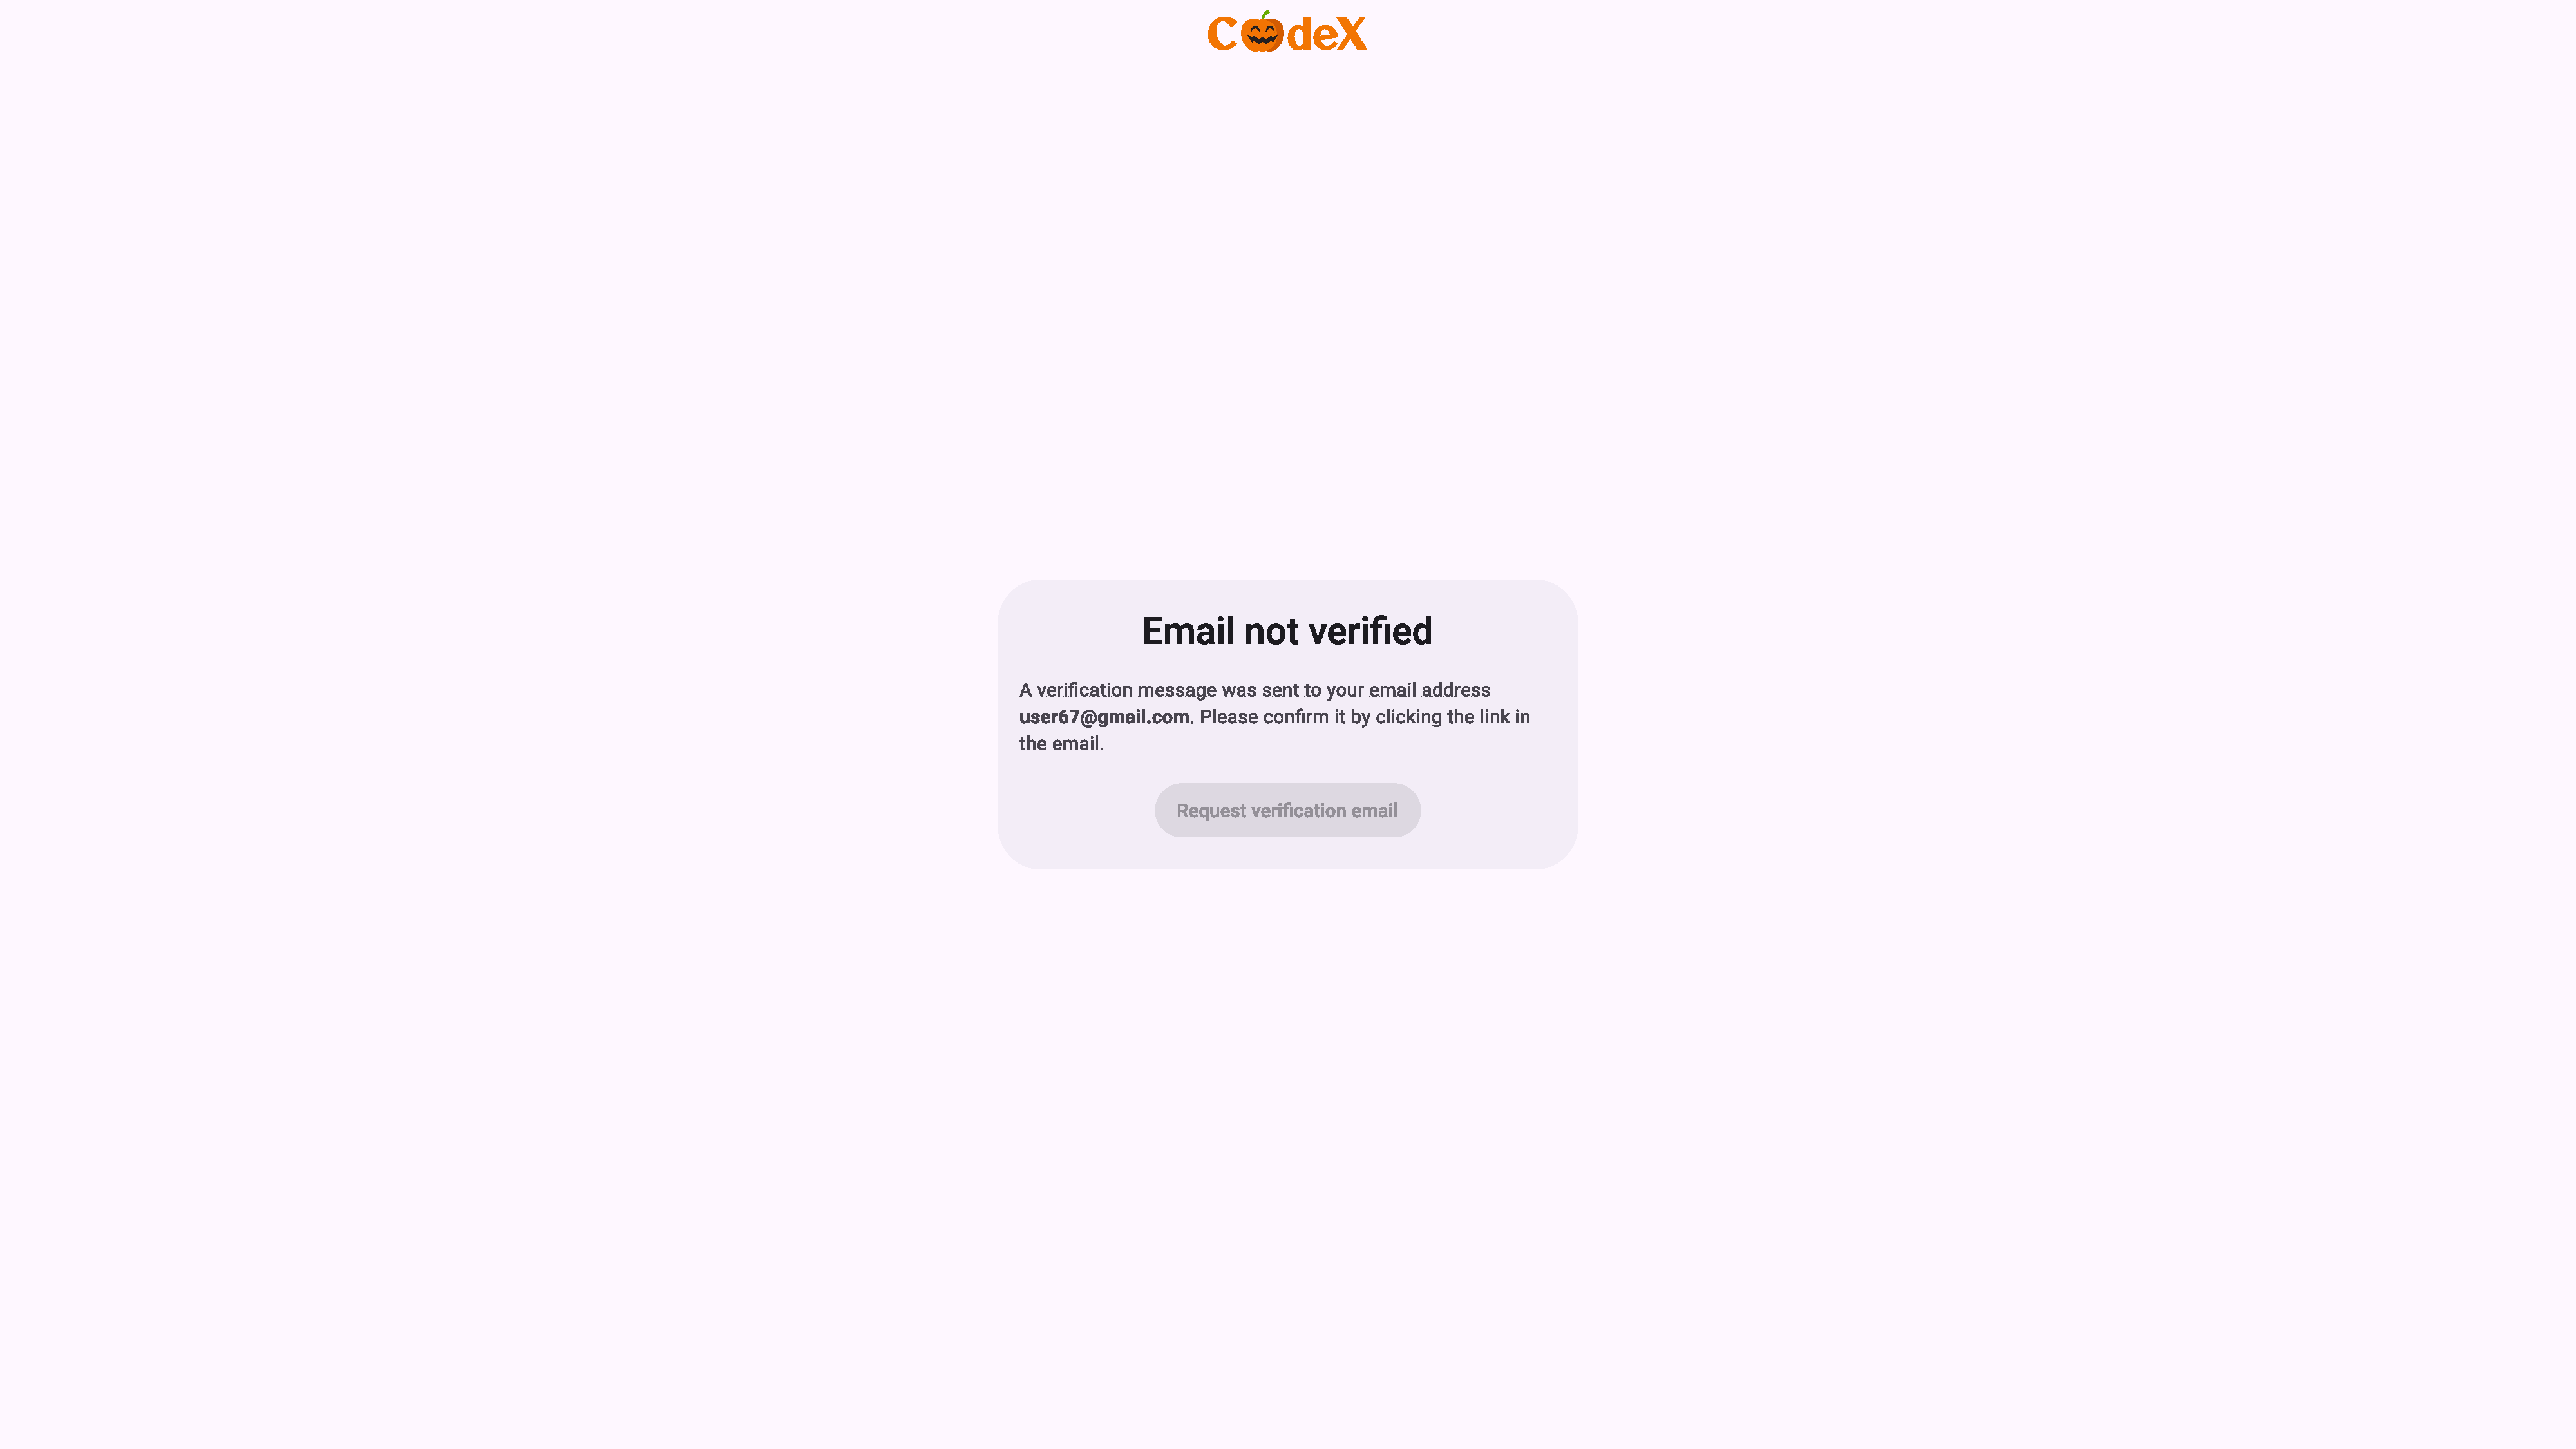
\includegraphics[width=\linewidth]{figures/ui/desktop/Not_Verified_Screen requested}
    \caption{\hyperref[abr:GUI]{GUI}: Not verified screen after requesting verification}
    \label{fig:ui-d-not-verified-requested}
\end{figure}
\begin{figure}
    \centering
    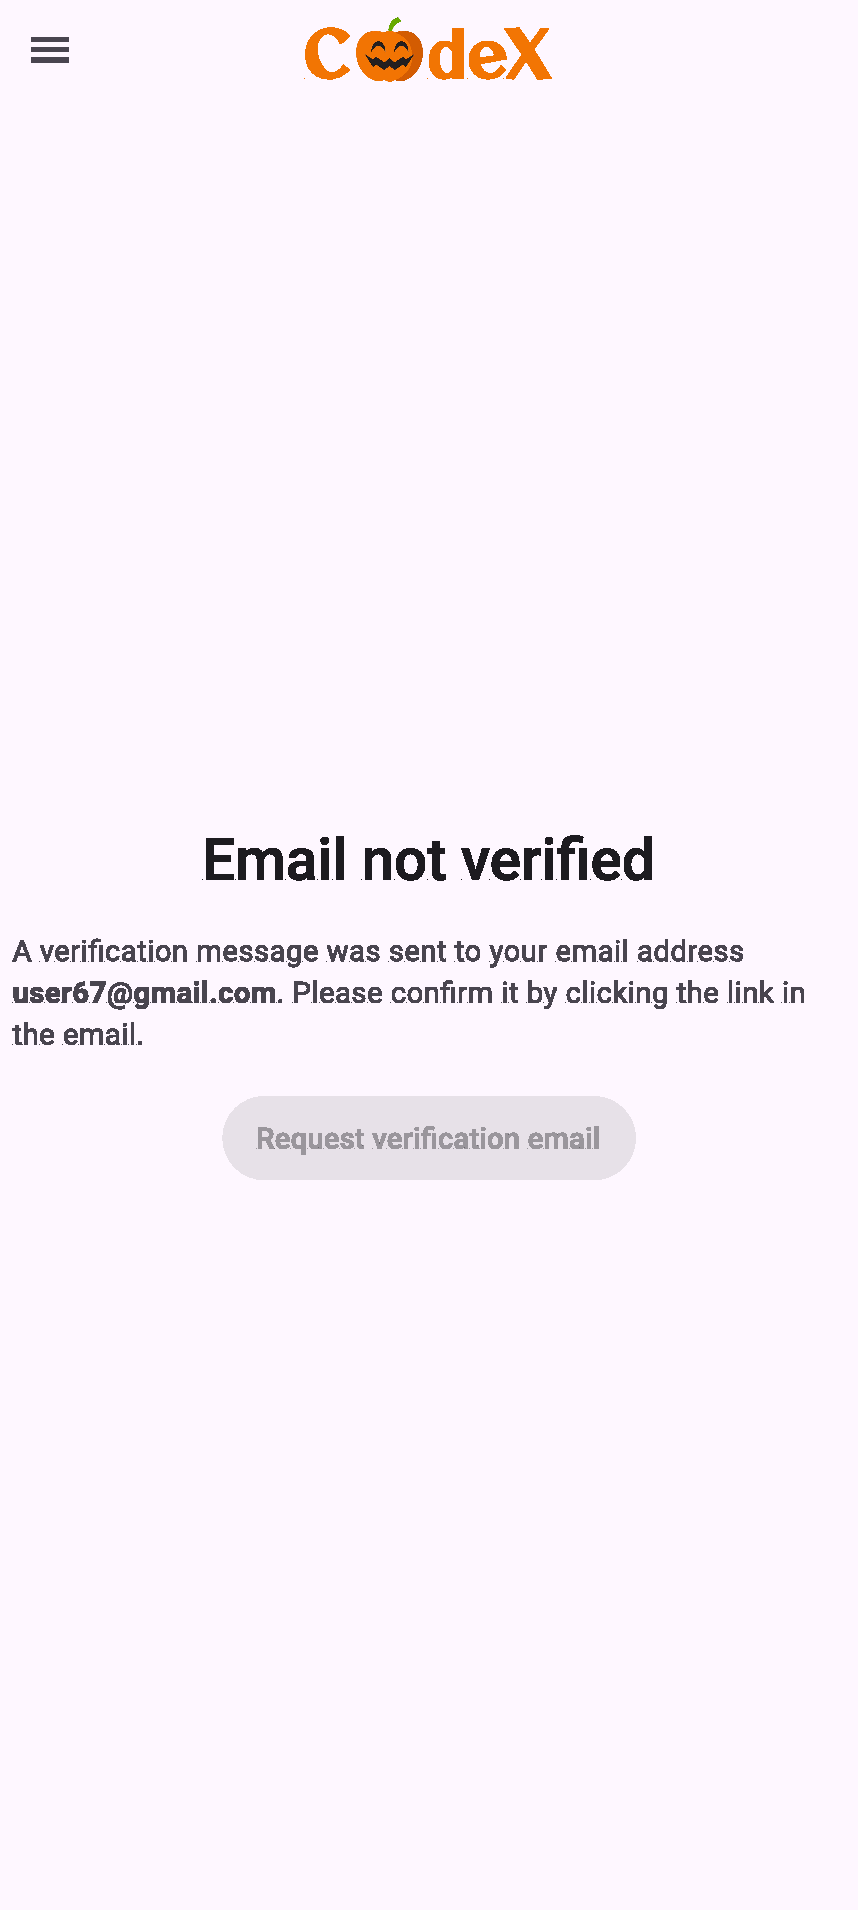
\includegraphics[width=5cm]{figures/ui/mobile/Not_Verified_Screen requested}
    \caption{\hyperref[abr:GUI]{GUI}: Not verified screen after requesting verification (mobile)}
    \label{fig:ui-m-not-verified-requested}
\end{figure}

\subsection{Verified screen}
The verified screen (\ref{fig:ui-d-verified}/\ref{fig:ui-m-verified}) is shown when the email of a user has been successfully verified.
This screen is shown after a user used the verification link in the message that was sent to them. \newline
\begin{figure}
    \centering
    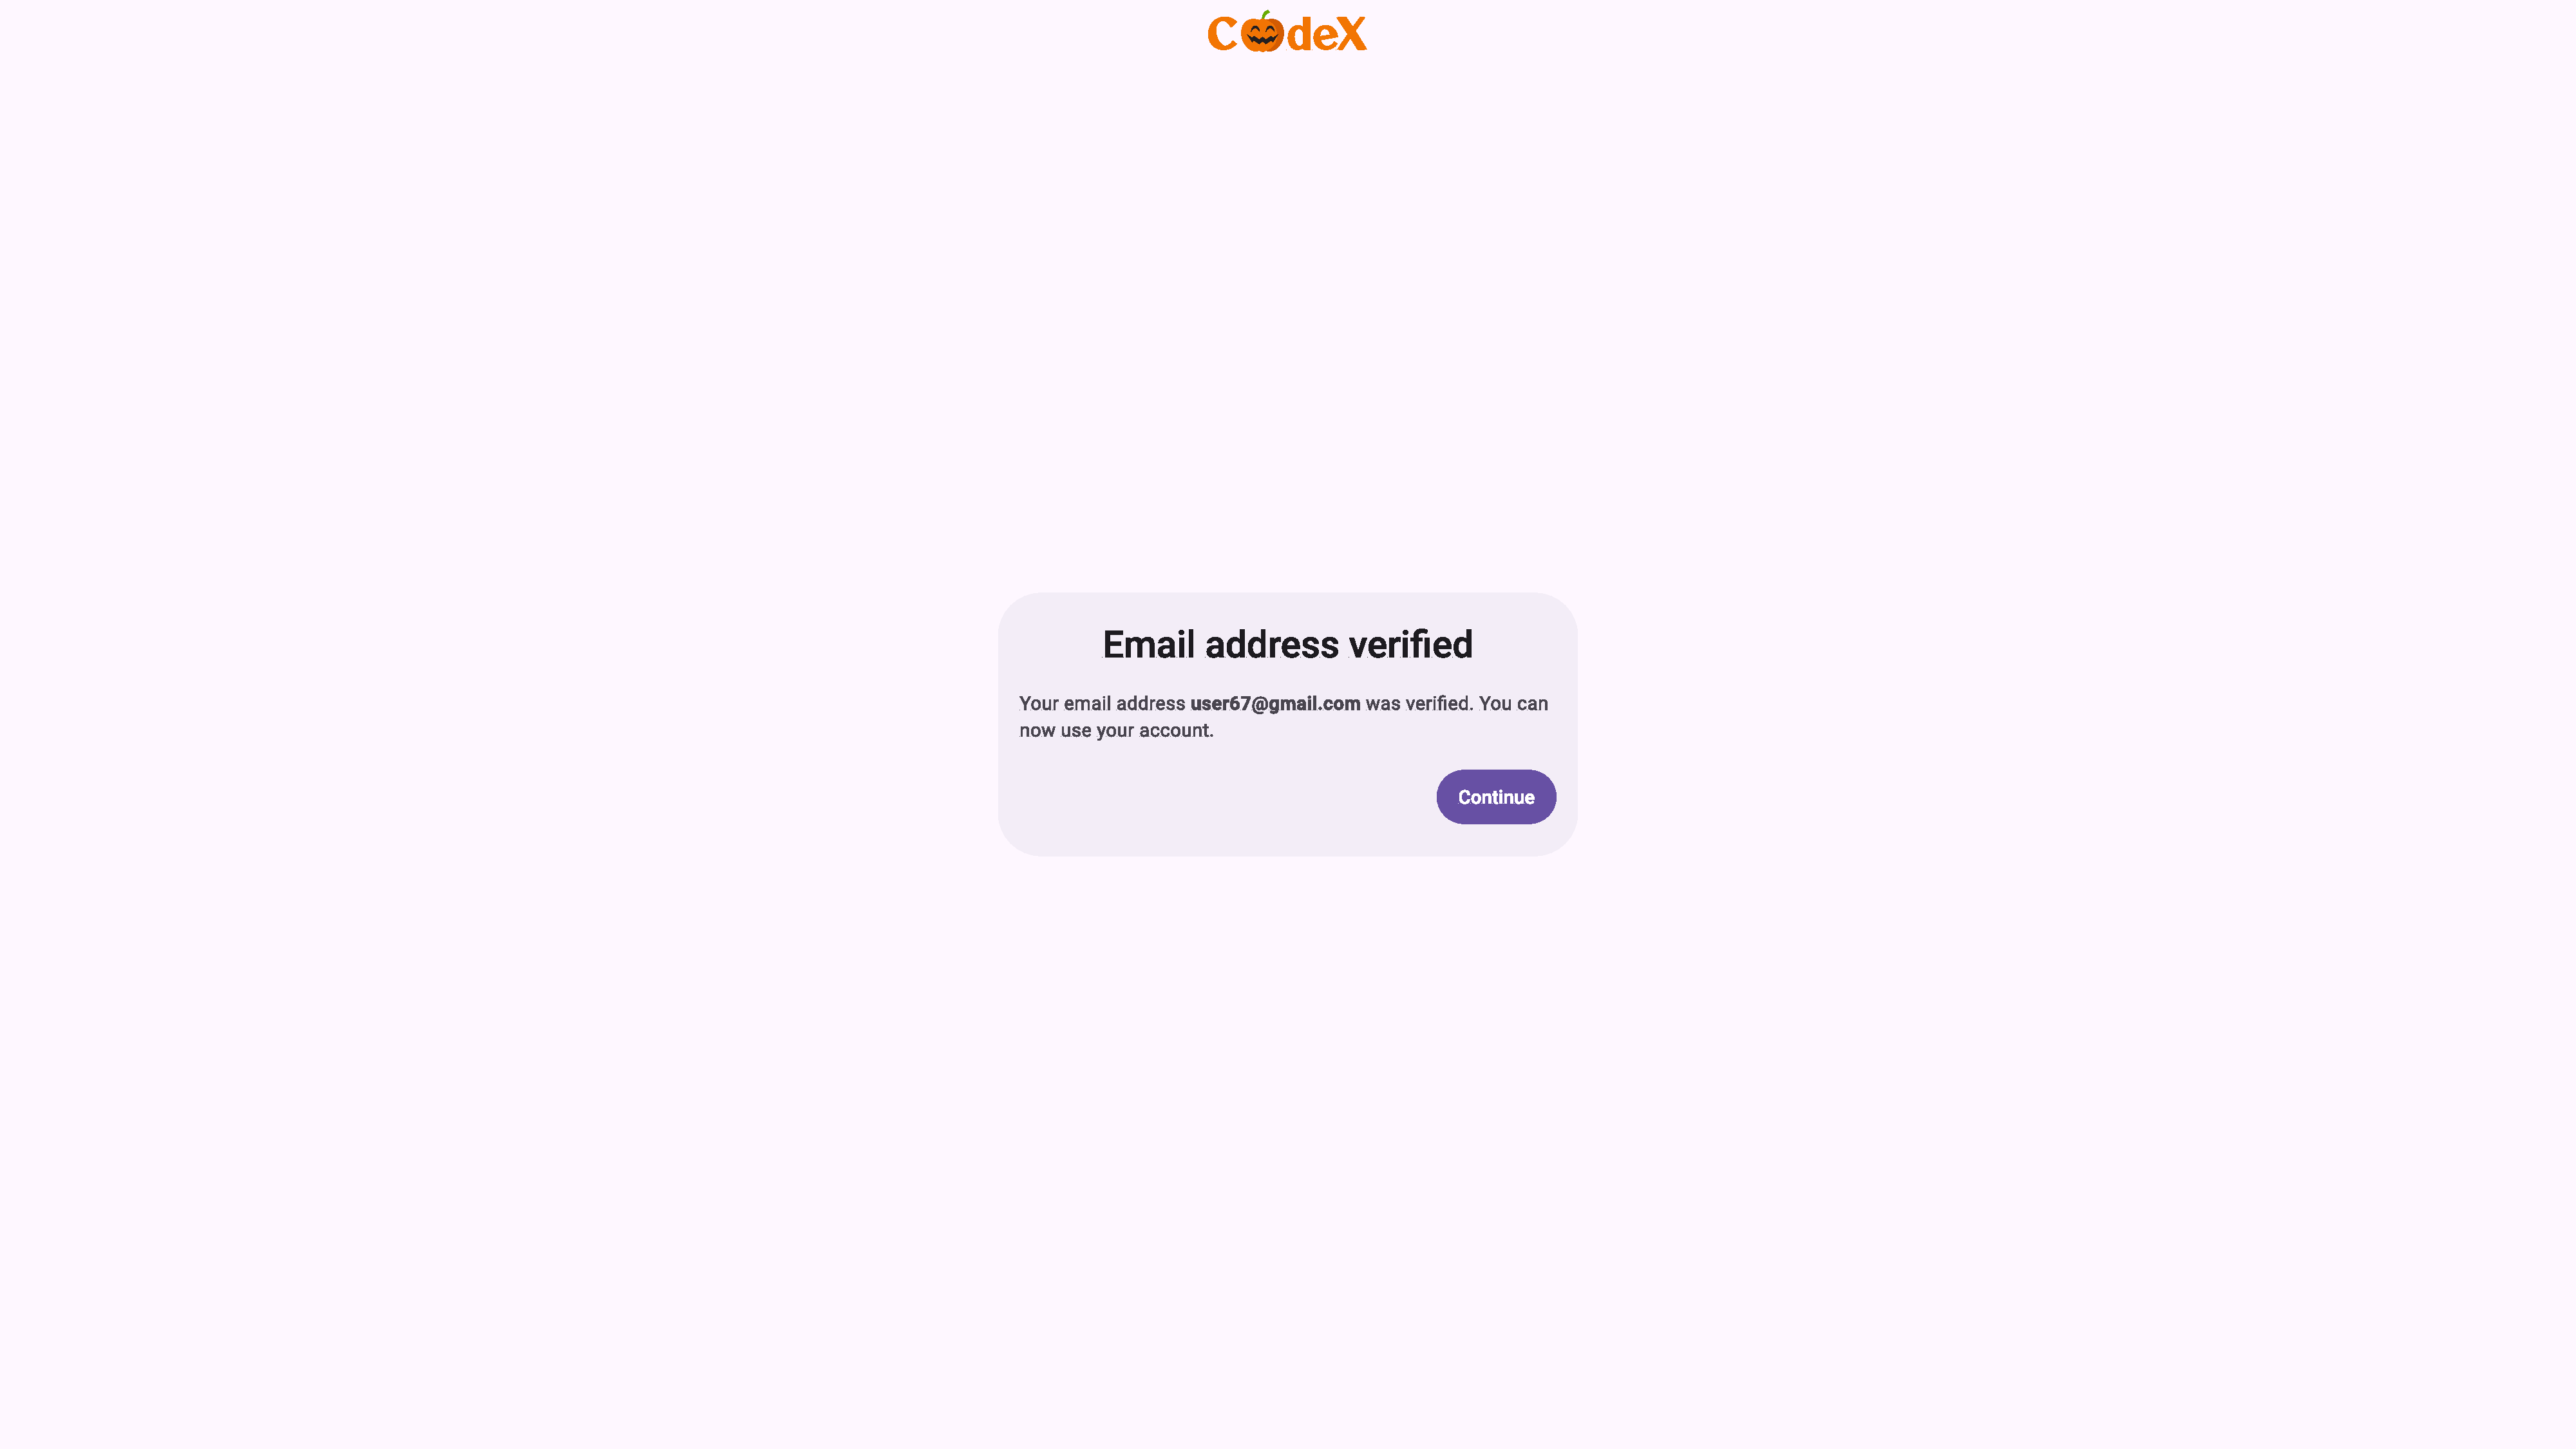
\includegraphics[width=\linewidth]{figures/ui/desktop/Email_Verification_Screen}
    \caption{\hyperref[abr:GUI]{GUI}: Verified screen}
    \label{fig:ui-d-verified}
\end{figure}
\begin{figure}
    \centering
    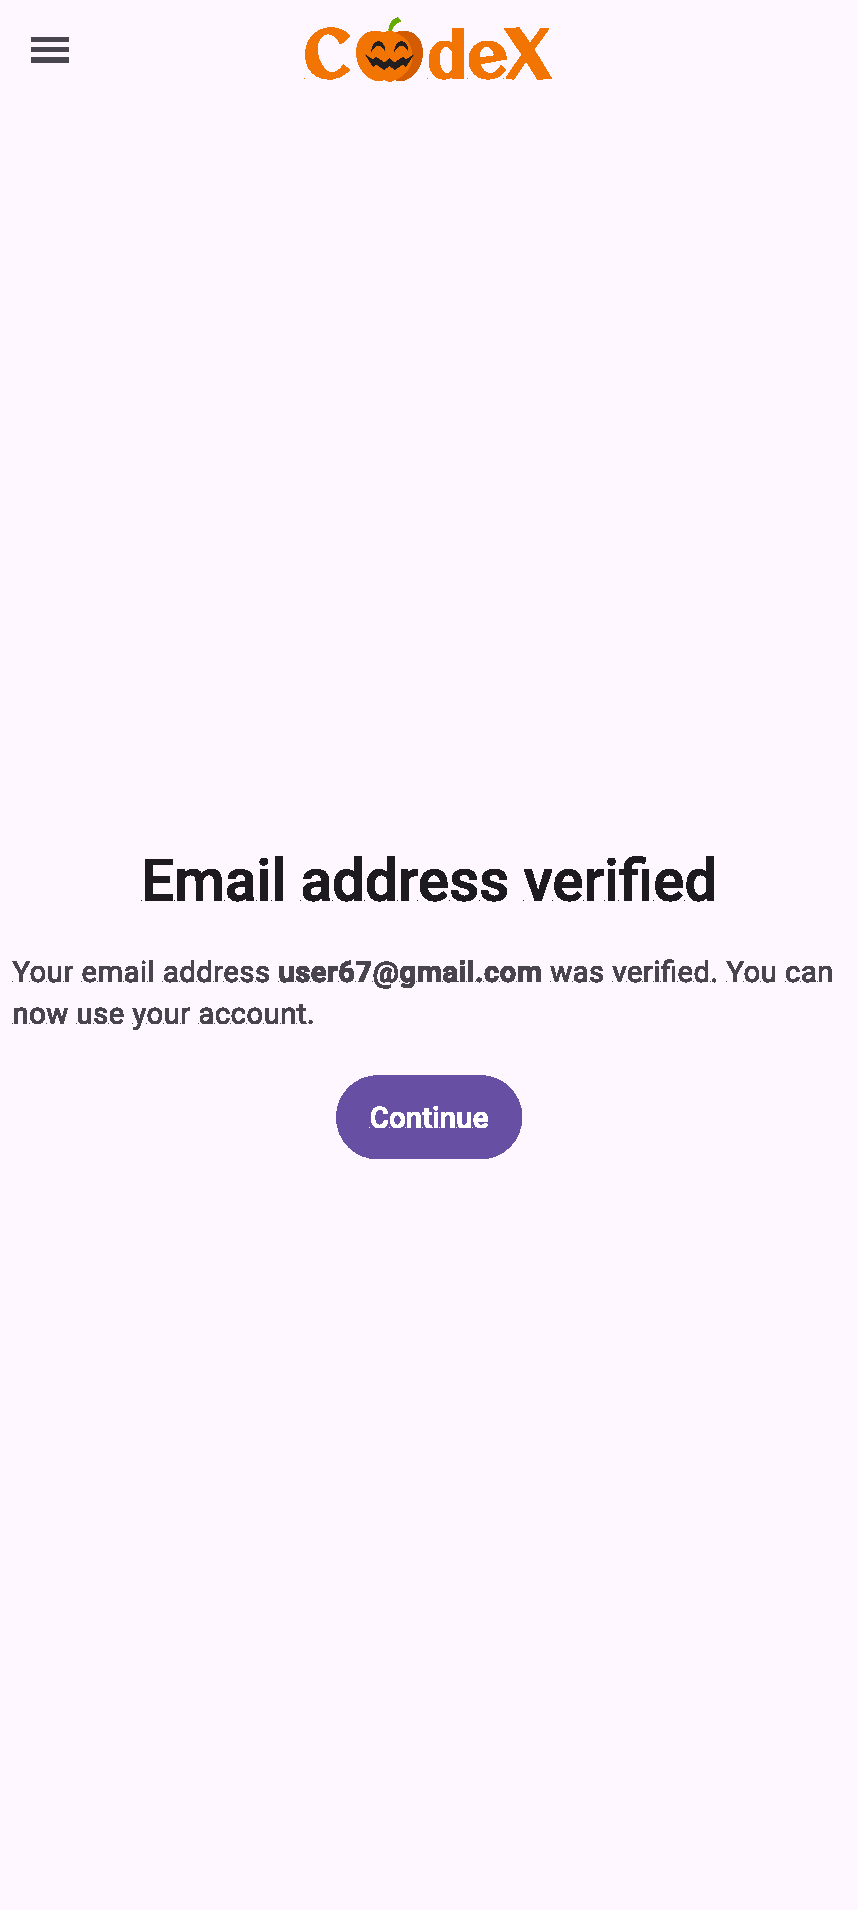
\includegraphics[width=5cm]{figures/ui/mobile/Email_Verification_Screen}
    \caption{\hyperref[abr:GUI]{GUI}: Verified screen (mobile)}
    \label{fig:ui-m-verified}
\end{figure}

\section{Modals}\label{sec:modals}
This section lists the modals, i.e. visual components that will be displayed as floating and over other components.
Namely, these are \textit{Dialog}s \footnote{https://m3.material.io/components/dialogs/overview} and \textit{Menu}s \footnote{https://m3.material.io/components/menus/overview}. \newline
These have the same layout and proportions on all screen sizes.

\subsection{Account dialog}
The account dialog is shown when users click the account settings button on the main screen. \newline
It displays information about the account, like username, email and current quota progress.
Actions like resetting the password or logging out are available. \newline
Depending on the role of the account, a dialog for  admin (\ref{fig:ui-d-account-dialog-admin}) or member (\ref{fig:ui-d-account-dialog-moderator}) is shown.
\begin{figure}
    \centering
    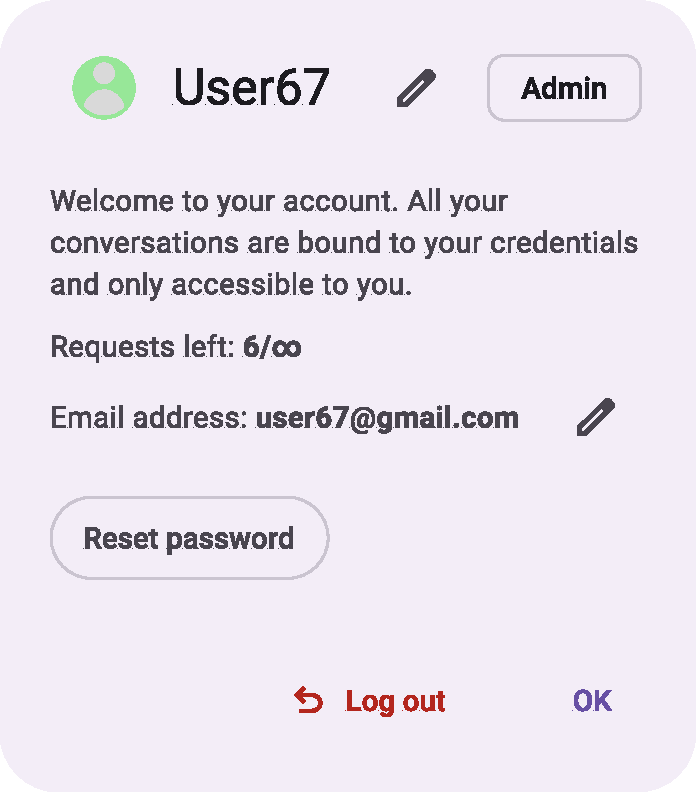
\includegraphics[width=5cm]{figures/ui/shared/Account_Dialog admin}
    \caption{\hyperref[abr:GUI]{GUI}: Account dialog for admin}
    \label{fig:ui-d-account-dialog-admin}
\end{figure}
\begin{figure}
    \centering
    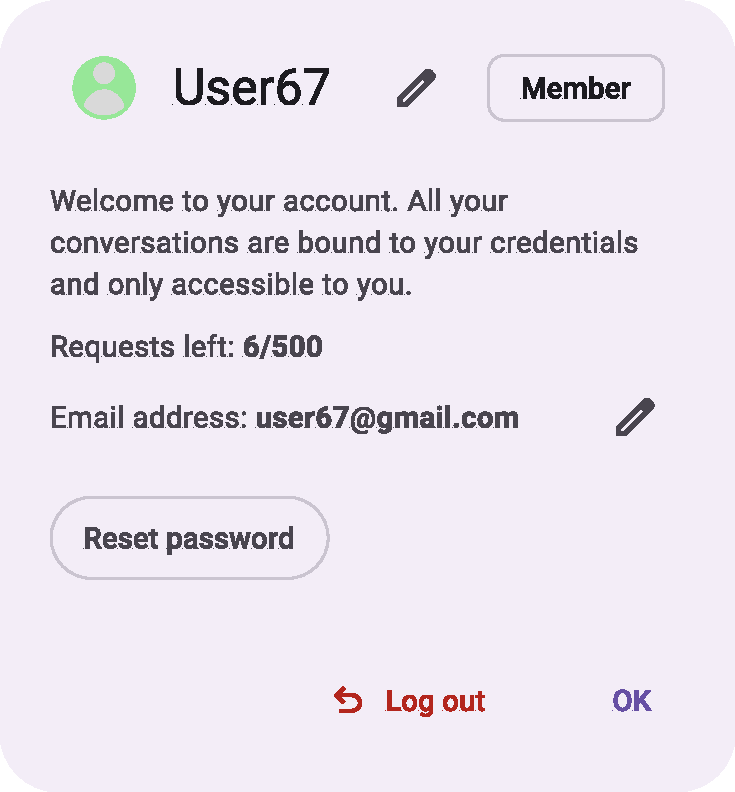
\includegraphics[width=5cm]{figures/ui/shared/Account_Dialog moderator}
    \caption{\hyperref[abr:GUI]{GUI}: Account dialog for user}
    \label{fig:ui-d-account-dialog-moderator}
\end{figure}

\subsection{Change username dialog}
The change username dialog (\ref{fig:ui-d-change-username-dialog}) allows a user to change the username of their account.
\begin{figure}
    \centering
    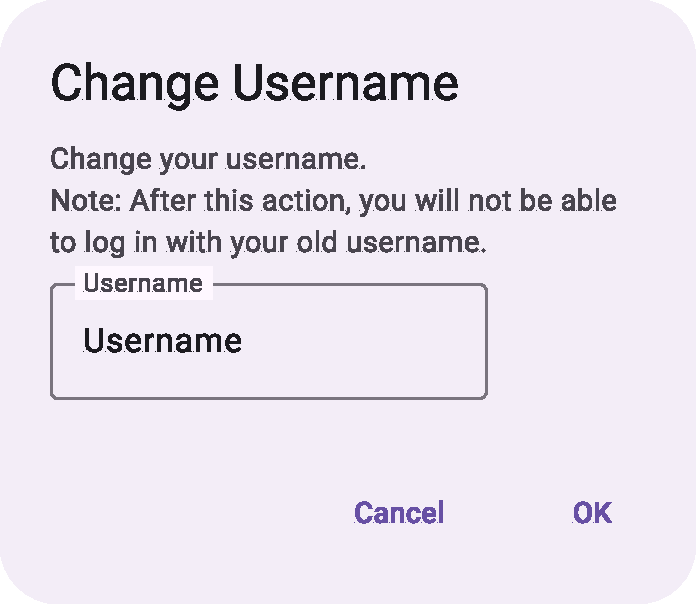
\includegraphics[width=5cm]{figures/ui/shared/Change_UsernameDialog}
    \caption{\hyperref[abr:GUI]{GUI}: Change username dialog}
    \label{fig:ui-d-change-username-dialog}
\end{figure}

\subsection{Change email dialog}
The change email dialog (\ref{fig:ui-d-change-email-dialog}) allows a user to change the email of their account. \newline
After the email was changed, the account is set to not verified again.
\begin{figure}
    \centering
    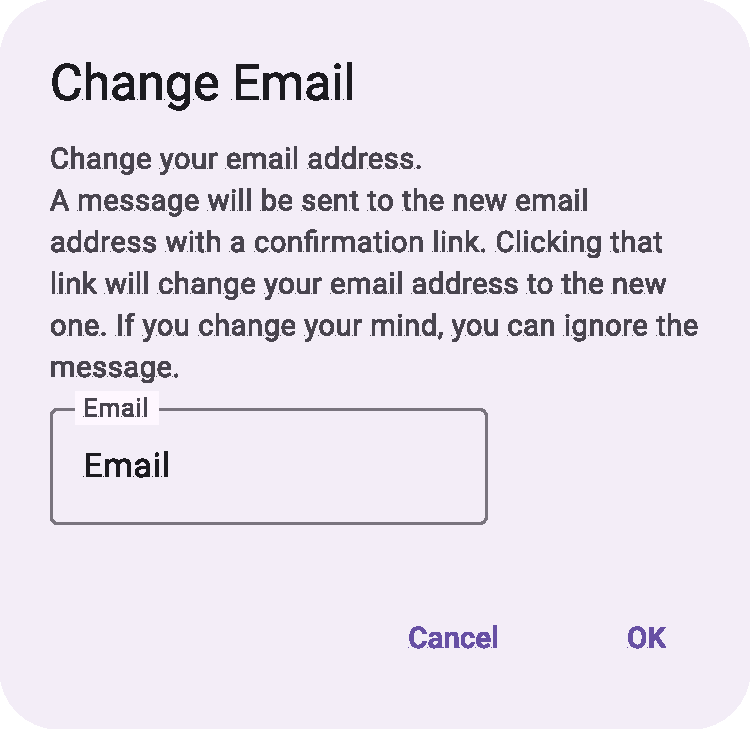
\includegraphics[width=5cm]{figures/ui/shared/Change_Email_Dialog}
    \caption{\hyperref[abr:GUI]{GUI}: Change email dialog}
    \label{fig:ui-d-change-email-dialog}
\end{figure}

\subsection{Conversation menu}
The conversation menu (\ref{fig:ui-d-conversation-menu}) is opened when the options button is clicked on a conversation item in the list of the main screen.
It allows a user to pin, rename or delete a conversation.
\begin{figure}
    \centering
    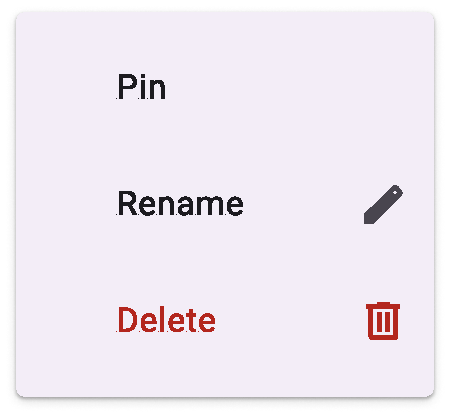
\includegraphics[width=3cm]{figures/ui/shared/Conversation_Menu}
    \caption{\hyperref[abr:GUI]{GUI}: Conversation menu}
    \label{fig:ui-d-conversation-menu}
\end{figure}
\section{Email}\label{sec:email}
In the following, we present the design for emails sent to the user. \newline
Due to the similar layout on mobile screens, the email-design is only presented for desktop devices.

\subsection{Password Reset Email}
Figure \ref{fig:ui_e_reset_password} shows the email sent to the user when the password is reset.
It contains a link to the web-interface.
\begin{figure}
    \centering
    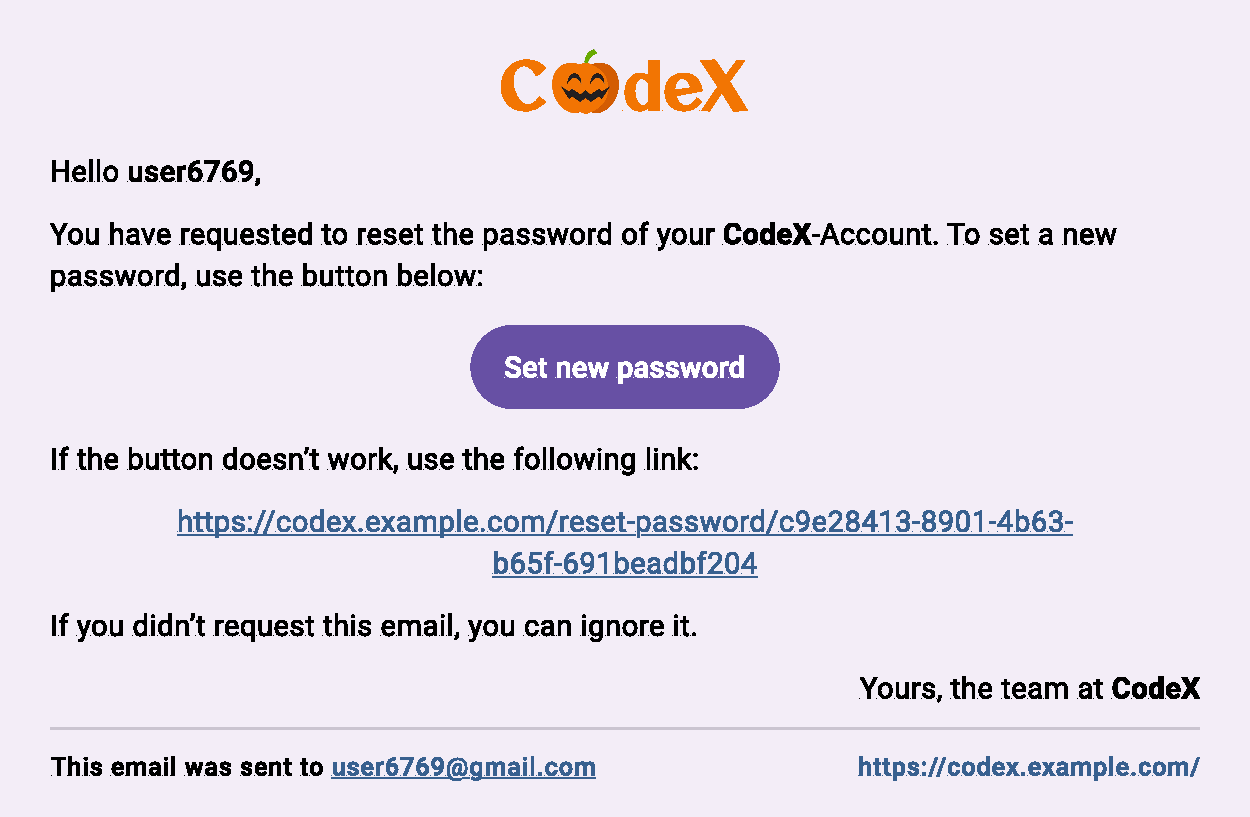
\includegraphics[width=\linewidth]{figures/ui/email/Password_Reset_Email}
    \caption{\hyperref[abr:GUI]{GUI}: Email for resetting password}
    \label{fig:ui_e_reset_password}
\end{figure}

\subsection{Email Verication Email}
Figure \ref{fig:ui_e_email_verify} shows the email sent to the user when their email needs to be verified.
It contains a link to the web-interface.
\begin{figure}
    \centering
    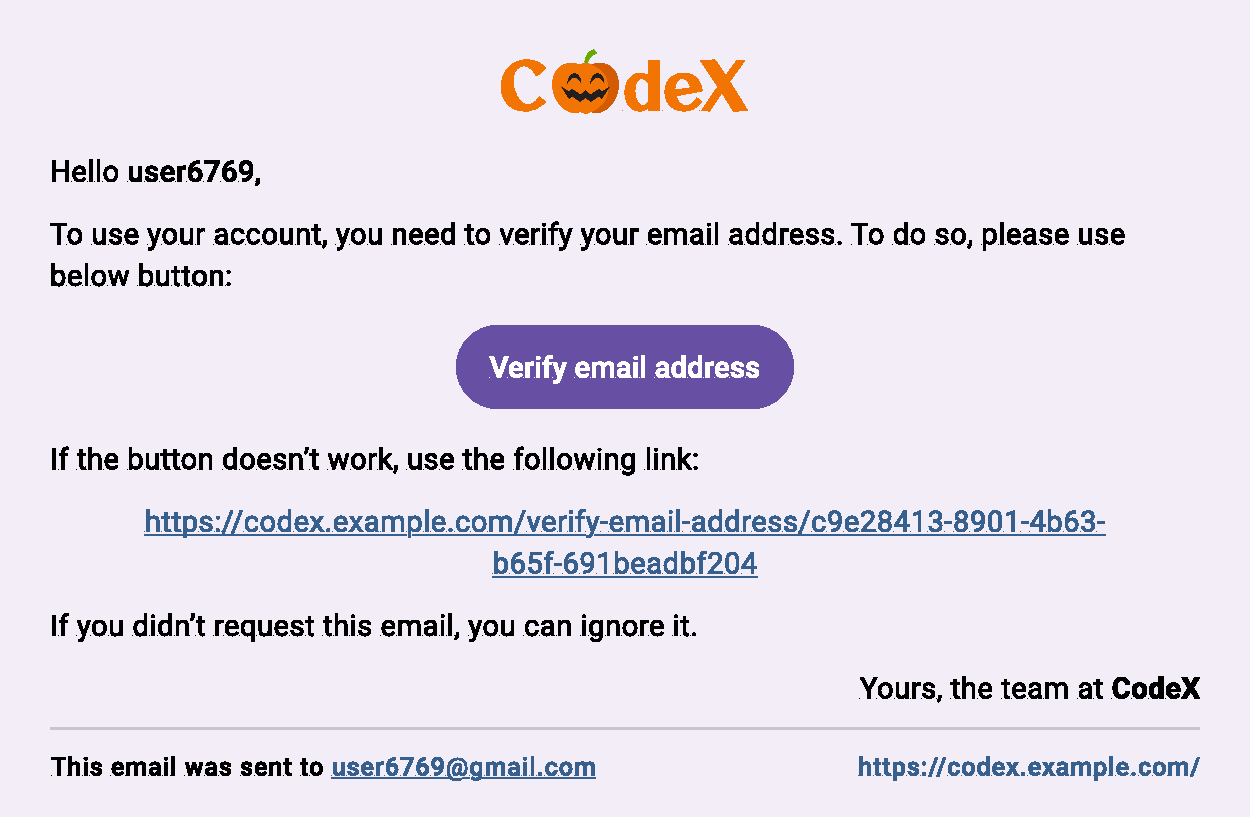
\includegraphics[width=\linewidth]{figures/ui/email/Email_Verify_Email}
    \caption{\hyperref[abr:GUI]{GUI}: Email for verifying email address}
    \label{fig:ui_e_email_verify}
\end{figure}
%!TEX root = ../Pflichtenheft.tex

% Kapitel 10
% Die Unterkapitel können auch in separaten Dateien stehen,
% die dann mit dem \include-Befehl eingebunden werden.
%-------------------------------------------------------------------------------

\chapter{Technical Product Environment}
\label{chap:tech_env}

This chapter describes the technical environment in which the product operates. It outlines the software architecture, technologies, and frameworks used for the implementation, as well as the tools and platforms that support development and deployment.

\section{Software}
The system is implemented in a \textbf{\hyperref[def:server-client]{Server-Client}} architecture, where the client application interacts with a centralized server to exchange data and perform operations.  
\subsection{Client}
The client component is a responsive single-page web-app that allows users to chat with an \hyperref[abr:AI]{AI} assistant, capable of generating code for a selection of \textit{\hyperref[abr:DSL]{DSL}s}, notably \textbf{\hyperref[abr:SPICE]{SPICE}}, based on a user prompt, and visualize generated code (if available). \newline
The client component will be developed using the  \textit{Angular Framework} \footnote{https://angular.dev/} with the \textit{Typescript} \footnote{https://www.typescriptlang.org/} programming language.

\subsection{Server}
The server component is a server that implements a \textit{\hyperref[abr:RAG]{RAG}} system and is programmed using the \textit{Python} \footnote{https://www.python.org/} programming language. \newline
The server component is connected to a \textit{Chroma} vector database for text embeddings, and a \textit{relational database} for storing app-specific data. The server component will use \textit{LangChain} and the \textit{Open\hyperref[abr:AI]{AI} \hyperref[abr:API]{API}} for communicating with the \textit{\hyperref[abr:LLM]{LLM}}.


\section{External interfaces}

\subsection{Graphical user interface}
The system will provide a \textit{Graphical user interface} (\hyperref[abr:GUI]{GUI}) as describes in~\ref{ch:ui}.
This \textit{\hyperref[abr:GUI]{GUI}} will be part of the client component and accessible via a browser. The interface enables users to: enter queries or prompts, view system responses or results, manage user-related actions such as login or session handling. The GUI enables users to enter prompts, view responses generated by the system, and manage application-specific features such as authentication or session control.

\subsection{Vector database}
The server component will interact with a \textit{\hyperref[def:vector-database]{Vector Database}} that will be used to store documents or specific \textit{\hyperref[abr:DSL]{DSL}} examples. Vector databases are used in \textbf{\hyperref[abr:RAG]{RAG}} systems to store vectorized text and query large amounts of documents based on similarity to a text snippet. Within this system, textual data is first transformed into high-dimensional vector embeddings, which are then indexed within the database. When a user submits a query, the system compares its embedding to stored vectors to identify the most semantically relevant information. This approach allows efficient handling of large text corpora and enhances the quality of responses provided by the language model.

\subsection{Large Language Model}
The server component will interact with a \textit{\hyperref[abr:LLM]{LLM}} that will provide the answers to the prompt provided by the user. This interaction enables the system to provide informative and context-aware answers that extend beyond simple pattern recognition.

\subsection{\hyperref[def:relational-database]{Relational Database}}
The server component will interact with a \textit{\hyperref[def:relational-database]{Relational Database}} (\hyperref[abr:RDB]{RDB}) to store application-specific data like user accounts, authentication tokens or conversations. 
\chapter{Test Cases}
\label{ch:test}

In the following, we will present functional test-cases that will be used as criteria to determine the functionality of the system, once implemented.

\begin{testcase}{10}{Authentication flow with OAuth provider}
  \item[Product functions]~\ref{F10},~\ref{F80}
  \item[Type of test] Functional test
  \item[Precondition] The user is not logged in.
  \item[Post-condition] The user is logged in
  \item[Execution] The user signs up via an OAuth provider (\ref{F10}), logs out (\ref{F80}) and then logs in via an OAuth provider (\ref{F10}).
\end{testcase}

\begin{testcase}{20}{Authentication flow with credentials}
  \item[Product functions]~\ref{F20},~\ref{F30},~\ref{F80}
  \item[Type of test] Functional test
  \item[Precondition] The user is not logged in.
  \item[Post-condition] The user is logged in
  \item[Execution] The user signs up via credentials (\ref{F20}), logs out (\ref{F80}) and then logs in via credentials (\ref{F30}).
\end{testcase}

\begin{testcase}{30}{Updating user data}
  \item[Product functions]~\ref{F40},~\ref{F50},~\ref{F60},~\ref{F70},~\ref{F90}
  \item[Type of test] Functional test
  \item[Precondition] The user is logged in with email $e_d$, username $u_d$, password $p_d$ and profile picture $p_d$
  \item[Post-condition] The user is logged in with email $e_n$, username $u_n$ and profile picture $p_d$
  \item[Execution] The user changed their email (\ref{F40}) to $e_n$ and verifies it (\ref{F50}).
    After that, the user resets their password (\ref{F60}) to $p_n$, username (\ref{F70}) to $u_n$ and profile picture (\ref{F90}) to $p_n$.
\end{testcase}

\begin{testcase}{40}{Making a request}
  \item[Product functions]~\ref{F100},~\ref{F110},~\ref{F120},~\ref{F170}
  \item[Type of test] Functional test
  \item[Precondition] The user is logged in and has available quota
  \item[Post-condition] The user is logged in, a request was created, the quota of the user has been decremented and the file has been exported.
  \item[Execution] The user selects the respective language model (\ref{F120}) and the target language (\ref{F110}).
    After that, the user makes the request (\ref{F100}). In the end, the user exports the code (\ref{F170}).
\end{testcase}

\begin{testcase}{50}{Manipulating language models}
  \item[Product functions]~\ref{F130},~\ref{F140}
  \item[Type of test] Functional test
  \item[Precondition] The user is logged in and has initially the language models $m_1 = (name_1, url_1)$ and $m_2 = (name_2, url_2)$
  \item[Post-condition] The user is logged in and has the language models $m_2 = (name_2, \hat{url_2})$ and $m_3 = (name_3, url_3)$
  \item[Execution] The user deletes the model $m_1$ (\ref{F140}).
    After that, the user updates the url of the language model $m_2$ from $url_2$ to $\hat{url_2}$ (\ref{F130}).
    Then, the user adds the language model $m_3 = (name_3, url_3)$.
\end{testcase}

\begin{testcase}{60}{Manipulating conversations}
  \item[Product functions]~\ref{F150},~\ref{F160},~\ref{F190},~\ref{F200}
  \item[Type of test] Functional test
  \item[Precondition] The user is logged in and has the conversations $c_1 = (n_1)$, $c_2 = (n_2)$, $c_3 = (n_3)$, of which $c_3$ is pinned.
  \item[Post-condition] The user is logged in and has the conversations $c_1 = (\hat{n_1})$, $c_2 = (n_2)$, of which $c_2$ is pinned.
  \item[Execution] The user renames conversation $c_1$ to $\hat{n_1}$ (\ref{F190}).
    After that, the user pins $c_2$ (\ref{F150}).
    Then, the user deletes $c_3$ (\ref{F200}).
\end{testcase}

\begin{testcase}{70}{Admin actions}
  \item[Product functions]~\ref{F210},~\ref{F220}
  \item[Type of test] Functional test
  \item[Precondition] The user is logged in as an admin and the current quota settings are $c = (c_1, c_2, c_3)$
  \item[Post-condition] The user is logged in as an admin and the current quota settings are $c = (\hat{c_1}, c_2, \hat{c_3})$
  \item[Execution] The user reads the current analytics (\ref{F220}).
    The, the user changes the quota settings to $c = (\hat{c_1}, c_2, \hat{c_3})$.
\end{testcase}

\begin{testcase}{80}{Change theme and language}
  \item[Product functions]~\ref{F180},~\ref{F230}
  \item[Type of test] Functional test
  \item[Precondition] The user is logged, the current theme is dark and the current language is \textit{German}.
  \item[Post-condition] The user is logged in, the current theme is light and the language of the user interface is \textit{English}.
  \item[Execution] The user toggles the theme (\ref{F180}) and changes its browser language settings to \textit{English} (\ref{F230}).
\end{testcase}

%!TEX root = ../Pflichtenheft.tex
\chapter{Glossary}

\section{Definitions}\label{sec:definitions}


\subsection{User-Roles}
\begin{description}[style=nextline, labelwidth=0pt, labelsep=0pt, leftmargin=0pt]
\setlength{\itemsep}{1em}
  \item[\textbf{\textit{User}}] \phantomsection\label{def:member}
    A registered and authenticated user with access to the system's core features.
    \item Users can view their request history, interact with personal data and perform a moderate number of requests.

  \item[\textbf{\textit{Admin}}] \phantomsection\label{def:admin}
    A privileged user with full administrative access to system settings.
    \item Admins can view system statistics and adjust configuration and quotas.

\end{description}

\newpage
\subsection{General Definitions}
\begin{description}[style=nextline, labelwidth=0pt, labelsep=0pt, leftmargin=0pt]
  \item[\textbf{\textit{OAuth}}] \phantomsection\label{def:oauth}
  OAuth (Open Authorization) is a standard authorization protocol that allows apps to access protected user data without having to share the user's log-in details (passwords). Instead, a temporary access token is used to authorize the user and determine which resources the app is allowed to use.

  \item[\textbf{\textit{RAG}}] \phantomsection\label{def:rag}
RAG is a framework for Retrieval-Augmented Generation, an \hyperref[abr:AI]{AI} approach that enhances large language models (\hyperref[abr:LLM]{LLMs}) by combining them with an external knowledge base. Instead of relying solely on their training data, \hyperref[abr:RAG]{RAG} models first retrieve relevant information from a specific source, such as a company's internal documents, before generating a response, leading to more accurate, up-to-date and contextually relevant answers without retraining the \hyperref[abr:LLM]{LLM}.
  
  \item[\textbf{\textit{Relational Database}}] \phantomsection\label{def:relational-database}
  A relational database is a type of database that organizes data into rows and columns, which collectively form a table where the data points are related to each other. Data is typically structured across multiple tables, which can be joined together via a primary key or a foreign key.

  \item[\textbf{\textit{Server-Client}}] \phantomsection\label{def:server-client}
  Server-Client architecture is a computing model where a client, such as a computer or app, sends a request to a central server for a service, data, or resource. The server processes this request and sends a response back to the client over a network, like the internet.

  \item[\textbf{\textit{SPICE}}] \phantomsection\label{def:spice}
  SPICE (Simulation Program with Integrated Circuit Emphasis) is a general-purpose, open-source analog electronic circuit simulator. It is used in integrated circuit and board-level design to check the integrity of circuit designs and predict circuit behavior.

  \item[\textbf{\textit{Vector Database}}] \phantomsection\label{def:vector-database}
  A vector database stores and queries data as high-dimensional vectors, which are numerical representations of complex data like text, images, or audio. Unlike traditional databases, it performs similarity searches to find data points that are mathematically "close" to a query vector, making it ideal for \hyperref[abr:AI]{AI} applications like semantic search and recommendation engines.
  
\end{description}
\newpage

\section{Abbreviations}\label{sec:abbreviations}
\begin{description}
\item[\textbf{AI}]\phantomsection\label{abr:AI} - Artificial Intelligence
\item[\textbf{API}]\phantomsection\label{abr:API} - Application Programming Interface
\item[\textbf{CI/CD}]\phantomsection\label{abr:CI/CD} - Continuous Integration/ Continuous Delivery
\item[\textbf{DSL}]\phantomsection\label{abr:DSL} - Domain Specific Language
\item[\textbf{GB}]\phantomsection\label{abr:GB} - Gigabyte
\item[\textbf{GUI}]\phantomsection\label{abr:GUI} - Graphical user interface
\item[\textbf{HTTP}]\phantomsection\label{abr:HTTP} - Hypertext Transfer Protocol
\item[\textbf{HTTPS}]\phantomsection\label{abr:HTTPS} - Hypertext Transfer Protocol Secure
\item[\textbf{IP}]\phantomsection\label{abr:IP} - Internet Protocol 
\item[\textbf{LLM}]\phantomsection\label{abr:LLM} - Large Language Model
\item[\textbf{Mbit/s}]\phantomsection\label{abr:Mbit/s} - Megabit per second
\item[\textbf{PII}]\phantomsection\label{abr:PII} - Personally Identifiable Information
\item[\textbf{PLC}]\phantomsection\label{abr:PLC} - Programmable Logic Controller
\item[\textbf{\hyperref[def:rag]{RAG}}]\phantomsection\label{abr:RAG} - Retrieval-Augmented Generation
\item[\textbf{RDB}]\phantomsection\label{abr:RDB} - Relational Database
\item[\textbf{SPA}]\phantomsection\label{abr:SPA} - Single Page Application
\item[\textbf{\hyperref[def:spice]{SPICE}}]\phantomsection\label{abr:SPICE} - Simulation Program with Integrated Circuit Emphasis
\item[\textbf{SQL}]\phantomsection\label{abr:SQL} - Structured Query Language
\item[\textbf{UI}]\phantomsection\label{abr:UI} - User Interface
\end{description}



%------Ende des Dokumentes------------------------------------------------------
\end{document}
